\documentclass[12pt,a4paper,twoside,openright,final]{memoir}
%draft / ms / final
%\usepackage[adobe-utopia]{mathdesign}
%\usepackage{kpfonts}
%\usepackage{mathptmx}
%\usepackage{fourier}
\usepackage[frenchb,english]{babel}
\usepackage[T1]{fontenc}
\usepackage[utf8]{inputenc}
\usepackage{lettrine}
\usepackage{yfonts}
\newcommand{\enluminure}[2]{\lettrine[lines=2]{\small \initfamily #1}{#2}}

\usepackage[inline]{enumitem}
\usepackage[babel=true,kerning=true]{microtype}
\usepackage{lipsum}
\usepackage[intlimits]{amsmath}
\usepackage{mathtools}

\usepackage[pdftex]{graphicx}
\newlength{\lofthumbsize}
\setlength{\lofthumbsize}{5em}

\newif\iflofimage
\DeclareRobustCommand*{\lofimage}[2][]{%
  \iflofimage
    $\vcenter to \lofthumbsize{\vss%
      \hbox to \lofthumbsize{\hss\includegraphics[{width=\lofthumbsize,height=\lofthumbsize,keepaspectratio=true,#1}]{#2}\hss}%
    \vss}$%
    \quad
  \fi
  \ignorespaces
}
\newcommand{\HRule}{\rule{\linewidth}{0.5mm}}
\usepackage{float}

\usepackage{fancybox}
\newenvironment{fminipage}%
{\begin{Sbox}\begin{minipage}}%
{\end{minipage}\end{Sbox}\fbox{\TheSbox}}

\newlength\drop

%% environnement infobox
\usepackage{etoolbox}
\newcounter{infobox}[section]
\renewcommand{\theinfobox}{\thechapter.\arabic{infobox}}
\usepackage[framemethod=TikZ]{mdframed}
\newenvironment{infobox}[1][]{%
    \refstepcounter{infobox}
    \begin{mdframed}[%
        frametitle={Box \theinfobox\ #1},
        skipabove=\baselineskip plus 2pt minus 1pt,
        skipbelow=\baselineskip plus 2pt minus 1pt,
        linewidth=2pt,
        frametitlerule=true,
        frametitlebackgroundcolor=gray!50,
        backgroundcolor=gray!10,
        roundcorner=7pt
    ]%
}{%
    \end{mdframed}
}
 
%% Euler for math | Palatino for rm | Helvetica for ss | Courier for tt
%\renewcommand{\rmdefault}{ppl} % rm
%%\linespread{1.05}        % Palatino needs more leading
%\usepackage[scaled]{helvet} % ss
%\usepackage{courier} % tt
%\usepackage{euler} % math
%%\usepackage{eulervm} % a better implementation of the euler package (not in gwTeX)
%\normalfont

% \pretolerance=1000
% \tolerance=1000 
% \emergencystretch=10pt


% bibliographie par chapitre :
%     * mettre \bibliography et \bibliographystyle dans chaque fichier inclu
%\usepackage[margin=1in]{geometry}
%\usepackage{parskip}
%\setlength{\parindent}{0pt}
%\nonzeroparskip
%\setlength{\parskip}{0.8cm plus4mm minus3mm}
\setlength{\headsep}{20pt}

%\usepackage[Sonny]{fncychap}
\addto\captionsfrench{\renewcommand{\chaptername}{Chapitre}}

\usepackage{titlesec}
%\usepackage{xcolor} 

%\titleformat{\chapter}[display]
%  {\normalfont\bfseries\LARGE}
%  {\chaptertitlename~\thechapter}{1pc}
%  {{\color{black}\titlerule[2pt]}\vspace{1pc}\MakeUppercase}
%\titleformat{name=\chapter,numberless}
%  {\normalfont\bfseries\LARGE}{}{1pc}
%  {\MakeUppercase}

\usepackage{csquotes}
\usepackage{kpfonts}
\usepackage{xcolor,calc, blindtext}
\definecolor{chaptercolor}{gray}{0.8}
% helper macros
\newcommand\numlifter[1]{\raisebox{-2cm}[0pt][0pt]{\smash{#1}}}
\newcommand\numindent{\kern37pt}
\newlength\chaptertitleboxheight
\makechapterstyle{hansen}{
  \renewcommand\printchaptername{\raggedleft}
  \renewcommand\printchapternum{%
    \begingroup%
    \leavevmode%
    \chapnumfont%
    \strut%
    \numlifter{\thechapter}%
    \numindent%
\endgroup%
}
  \renewcommand*{\printchapternonum}{%
    \vphantom{\begingroup%
      \leavevmode%
      \chapnumfont%
      \numlifter{\vphantom{9}}%
      \numindent%
      \endgroup}
    \afterchapternum}
  \setlength\midchapskip{0pt}
  \setlength\beforechapskip{0.5\baselineskip}
  \setlength{\afterchapskip}{3\baselineskip}
  \renewcommand\chapnumfont{%
    \fontsize{4cm}{0cm}%
    \bfseries%
    \sffamily%
    \color{chaptercolor}%
  }
  \renewcommand\chaptitlefont{%
    \normalfont%
    \huge%
    \bfseries%
    \raggedleft%
  }%
  \settototalheight\chaptertitleboxheight{%
    \parbox{\textwidth}{\chaptitlefont \strut bg\\bg\strut}}
  \renewcommand\printchaptertitle[1]{%
    \parbox[t][\chaptertitleboxheight][t]{\textwidth}{%
      %\microtypesetup{protrusion=false}% add this if you use microtype
      \chaptitlefont\strut ##1\strut}%
}}
\chapterstyle{hansen}
\aliaspagestyle{chapter}{empty} % just to save some space

%\chapterstyle{ell}




\DoubleSpacing
%\OnehalfSpacing

\usepackage[natbib=true,maxcitenames=2,maxbibnames=99,style=authoryear-comp,backend=biber,
doi=false, isbn=false, url=false]{biblatex}
% \renewbibmacro*{name:andothers}{% Based on name:andothers from biblatex.def
%   \ifboolexpr{
%     test {\ifnumequal{\value{listcount}}{\value{liststop}}}
%     and
%     test \ifmorenames
%   }
%     {\ifnumgreater{\value{liststop}}{1}
%        {\finalandcomma}
%        {}%
%      \andothersdelim\bibstring[\emph]{andothers}}
%     {}}
%\usepackage{biblatex-chicago}
% \addbibresource{allbiblio.bib}
% \addbibresource{BPSensor.bib}
% \addbibresource{STdiag.bib}
% \addbibresource{FIP.bib}
\addbibresource{Biblio/MergedBib.bib}

%\bibliography{allbiblio.bib}

\usepackage{tabularx}
\usepackage{multirow}
\usepackage{subfig}
\usepackage{caption}
\usepackage{subfig}
\usepackage{float}
\usepackage{subfloat}
\usepackage{longtable}
\usepackage{tabu}
\renewcommand{\arraystretch}{0.75}

\makeatletter
\providecommand\phantomcaption{\caption@refstepcounter\@captype}
\makeatother

\setsecnumdepth{subsection}
\settocdepth{subsection}
\semiisopage[12]
\usepackage[hidelinks]{hyperref}

\settrimmedsize{297mm}{210mm}{*}
\setlength{\trimtop}{0pt}
\setlength{\trimedge}{\stockwidth}
\addtolength{\trimedge}{-\paperwidth}
\settypeblocksize{634pt}{448.13pt}{*}
\setulmargins{4cm}{*}{*}
\setlrmargins{*}{*}{1.5}
\setmarginnotes{17pt}{51pt}{\onelineskip}
\setheadfoot{\onelineskip}{2\onelineskip}
\setheaderspaces{*}{2\onelineskip}{*}
\checkandfixthelayout

\makeheadrule{headings}{\textwidth}{\normalrulethickness}

\addto{\captionsenglish}{\renewcommand{\abstractname}{Résumé}}
\addto{\captionsenglish}{\renewcommand{\partname}{Partie}}
\addto{\captionsenglish}{\renewcommand{\chaptername}{Chapitre}}
\addto{\captionsenglish}{\renewcommand{\contentsname}{Table des matières}}
\addto{\captionsenglish}{\renewcommand{\listfigurename}{Liste des figures}}
\addto{\captionsenglish}{\renewcommand{\listtablename}{Liste des tables}}
\addto{\captionsenglish}{\renewcommand{\tablename}{Liste des tableaux}}

\usepackage{tocloft}
\setlength{\cftpartnumwidth}{2.0em}
\setlength{\cftchapternumwidth}{2.2em}
\setlength{\cftsectionnumwidth}{3.2em}
% \makeatletter
% \renewcommand{numberline}[1]{%
%  \@cftbsnum #1\@cftasnum~\@dftasnumb%
% }
% \makeatother

%\usepackage{chngcntr}
%\numberwithin{chapter}{part}

% \makeatletter
% \@addtoreset{chapter}{part}
%	\renewcommand{\l@chapter}{l@dottedtocline{1}{1.5em}{2.6em}}

%#############	Select files to compile
%\includeonly{1_CorpsDeThese/Intro}
%#############

\title{Manuscrit de thèse}

\begin{document}
%d�but du doc
\frontmatter

% le titre
% Page de titre 

\begin{titlingpage}
\selectlanguage{french}
\begin{Spacing}{1}
\begin{center}     

% Upper part of the page 
\includegraphics[width=0.3\textwidth]{0_Title/upmc.png}\hfill
\includegraphics[width=0.4\textwidth]{0_Title/LogoLabo.png}\\[1cm]
 
 \vspace{2cm}
 
\begin{Spacing}{1.5}
\textsc{\LARGE THÉSE PRÉSENTÉE À L'UNIVERSITÉ PIERRE ET MARIE
CURIE}\\[0.8cm]

\textsc{ÉCOLE DOCTORALE DIVERSITÉ DU VIVANT}
\end{Spacing} 
\vfill

% Author and supervisor 
\emph{Par}\\ 
Vincent \textsc{Le Bourlot} \vfill
\textsc{Pour obtenir le grade de docteur} de l'Université Pierre et Marie
Curie\\
\textsc{Spécialité}: \'Ecologie\\

\vfill


% Title 
\HRule \\[0.2cm] 
{\textbf{\LARGE\textsc{Compétition par interférence, température et dynamique
des populations structurées}\\[0.7cm] \Large Etude expérimentale et théorique
chez le Collembole \textit{Folsomia candida}}}\\[0.2cm] \HRule \\ 

\vfill
\end{center} 
% Author and supervisor 
Soutenue à Paris le 16 Mai 2014.\\
\vfill

\begin{flushleft}
\begingroup
    \fontsize{11pt}{12pt}\selectfont


\begin{tabularx}{1.03\textwidth}{Xl}
Sous la direction de: &\\
&\\
Dr. \textbf{David \textsc{Claessen}}, Maître de conférence à l'Ecole Normale
Supérieure & \\
Dr. \textbf{Thomas \textsc{Tully}}, Maître de conférence à l'Université
Paris-Sorbonne & \\
&\\
Devant le jury composé de: & \\
& \\
Pr. \textbf{Amaury \textsc{Lambert}}, Professeur à l'Université Pierre
et Marie Curie & Président du jury \\
Pr. \textbf{André M. \textsc{de Roos}}, Professeur à l'Université d'Amsterdam &
Rapporteur \\
Dr. \textbf{Ophélie \textsc{Ronce}}, Chargée de recherche l'Université de
Montpellier 2 & Rapportrice \\
Pr. \textbf{Jean-Christophe \textsc{Poggiale}}, Professeur à l'Université
d'Aix-Marseille & Examinateur\\
Dr. \textbf{Bruno \textsc{Ernande}}, Cadre de recherche à l'Ifremer &
Examinateur
\\
\end{tabularx}

\endgroup
\end{flushleft}
\end{Spacing}
 

\end{titlingpage}

%\newgeometry{left=1in,right=1.5in,top=1.2in,bottom=1.2in}

% table des matieres generale
\begin{Spacing}{1}

\begin{abstract}
De plus en plus reconnue comme jouant un rôle majeur dans la régulation des
populations, la compétition par interférence et ses effets sur la dynamique des
populations suscitent un intérêt croissant. De plus, la température est connue
comme facteur abiotique ayant un fort impact sur la physiologie et les
comportements individuels ainsi que sur les dynamiques des populations.

Dans un contexte de réchauffement planétaire, comprendre comment les
interactions directes entre les individus se répercutent sur la dynamique
globale d’une population et comment cela interagit avec l’effet de la
température constitue un enjeu important pour la biologie des populations.

Les interactions interindividuelles étant fortement liées à la taille corporelle
des individus, la structure en taille de plusieurs populations de deux lignées
clonales du collembole Folsomia candida a été finement suivie pendant deux à
quatre ans à six températures de 6$\degres$C à 26$\degres$C. Une première analyse des séries
temporelles de la structure des populations à 21$\degres$C a révélé une dépendance forte
de la structure des populations et de sa dynamique aux conditions d’accès de
chaque individu à la ressource, liées notamment à la présence d’individus
adultes de grande taille. Nous avons ensuite modifié artificiellement la
structure de plusieurs populations en isolant certaines classes de taille dans
des populations séparées, et observé le retour à l’équilibre de la structure en
taille. Parallèlement, nous avons observé en temps réel le comportement d’accès
à la ressource. Ces études ont permis de montrer le rôle déterminant joué par la
présence d’adultes de grande taille dans la régulation de la population en
interférant avec les individus plus petits et en monopolisant la ressource.

La compétition par interférence a donc été implémentée dans un modèle théorique
de dynamique des populations structurées pour étudier l’impact du niveau
d’interférence sur la dynamique d’une population. Nous avons montré que
l’intensité de l’interférence peut avoir des effets variés sur la dynamique
d’une population structurée, tels que stabiliser des cycles de générations,
permettre la survie d’individus de très grande taille, et causer une
déstabilisation vers des cycles de très grande période et amplitude.

Nous avons ensuite comparé des normes de réactions à la température sur des
individus isolés et dans les populations suivies afin de comprendre comment la
compétition interagit avec la température dans la régulation de la dynamique de
la population. Ceci a également permis de montrer la nécessité d’englober
plusieurs niveaux de complexité pour comprendre comment des changements
environnementaux peuvent se répercuter sur la dynamique des populations. Cette
étude a enfin servi de base à une intégration de la température dans le modèle
précédemment développé afin d’étudier d’un point de vue théorique les
interactions entre température et compétition.

\vspace{1pt}

Mots clés: Collembole, dynamique des populations, populations structurées,
compétition, exploitation, interférence, modèles physiologiquement structurés,
température, norme de réaction

\end{abstract}

%\tableofcontents

%\setlength{\parskip}{0.0pt plus 1.0pt}

\tableofcontents

\end{Spacing}
%\setlength{\parskip}{0.8cm plus4mm minus3mm}


%d�but du texte
\mainmatter
% inclusion des chapitres

\title{Compétition par interférence, température et dynamique des populations
structurées : \'Etude expérimentale et théorique chez le Collembole
\textit{Folsomia candida}}
\newpage
\selectlanguage{french}
\part{Introduction Générale}

\chapter{Introduction}

\chapter{État de l'art}

\section{Les conséquences écologiques de la structuration des populations}

\lettrine[lines=3]{P}{our comprendre} le fonctionnement des écosystèmes et les
réponses des espèces à leur environnement, il est d'important de comprendre leur démographie et la
dynamique de leur populations. De nombreuses études empiriques ont montré que
ces populations étaient structurées de façon non triviales. C'est un 
résultat très général qui a été vérifié à de nombreuses reprises, que ce soit en
laboratoire, comme chez la drosophile ou chez des acariens par exemple, ou dans
des populations naturelles telles que les populations de moutons de Soay ou de cerfs
élaphe. 
Cela implique que la description d'une population comme un tout ou comme
un assemblage de classe crées artificiellement représente généralement mal la
réalité et n'intègre pas suffisamment de complexité pour décrire fidèlement les
mécanismes qui régulent sa dynamique.

\subsection{Différents niveaux de structuration}

Dans une population, la structure émerge de l'hétérogénéité entre les
individus d'une même espèce. Plusieurs formes de structures ont été
classiquement prises en compte en écologie.

\subsubsection{Structuration spatiale}

Une première forme de structuration évidente est la structuration spatiale. Ceci
décrit comment les individus d'une population s'organisent dans l'espace, et ce
faisant, modifient leurs interactions entre eux et avec leur environnement. 

La structuration spatiale des populations répond souvent à l'hétérogénéité de
leur habitat. Ces hétérogénéités ont des conséquences directes sur la dynamiques
des populations, par exemple en modifiant les schémas de dispersion des
individus \autocite{hiebeler2000a}, leur fitness \autocite{zajkac2008a},
l'accès aux ressources \autocite{burger2008a}, la sensibilité aux parasite ou
pathogènes \autocite{su2009a}, \textit{etc}.

L'étude de la dynamique des populations structurées spatialement constitue un
champs de recherche extrêmement large et varié auquel notre étude ne se rattache
pas directement. 

\subsubsection{Structuration génétique}

Conséquence de la structuration spatiale, les population sont souvent également
structurées génétiquement. Les individus les plus proches les uns des autres,
notamment dans des méta-populations, sont également plus proches génétiquement
que des individus spatialement éloignés. L'analyse génétique d'une population
permet alors d'obtenir des informations sur ses origines et sa structuration
spatiale \autocite{repaci2006a,booth2009a,jorde2007a}.

\subsubsection{Structuration en stades}
\subsubsection{Structuration en âges}
\subsubsection{Structuration physiologique}

\subsection{Importance de la taille corporelle}

\subsubsection{Sur les traits d'histoire de vie}

\subsubsection{Sur la structure et la dynamique des populations}

\subsubsection{Sur la structure et la dynamique des communautés}





% Une des causes principales de cette hétérogénéité
% vient du cycle de vie de l'espèce et des différentes étapes qu'un individu
% traverse au cours de ce cycle. 

\section{Mécanismes de densité dépendance}

\section{Le rôle de la température}

\section{Problématiques}	


\chapter{Éléments de méthodologie}

Le travail présenté dans cette thèse repose sur de travaux expérimentaux et
théoriques. En particulier, la partie expérimentale a été centrée sur l'étude de
populations de Collemboles de l'espèce \textit{Folsomia candida} élevée en
microcosmes au laboratoire. Dans ce chapitre, nous présenterons notre espèce
modèle du point de vu de sa biologie, de son intérêt pour les études menées, et
des conditions d'élevages. Puis nous détaillerons quelques développements
méthodologique qui ont permis l'accomplissement de nos travaux. 

\section{Le collembole, un modèle d'étude en écologie des populations}
\sectionmark{Le collembole modèle d'étude}

\subsection{Quelques généralités}

les Collemboles sont de petits arthropodes hexapodes entognathes aptères
mesurant généralement 1 à 5 mm. C'est un groupe très anciens qui compte
notamment l'un des plus vieux fossiles d'héxapode connu (\textit{Rhyniella
praecursor}). Aujourd'hui, plus de 8000 espèces ont été décrites
\autocites{bellinger2014a}, réparties dans l'ensemble des écosystèmes connus, en
faisant une des lignées d'arthropodes les plus communes au monde. Bien que
proches des Insectes, les Collemboles forment une classe à part, à côté des
Diploures, des Protoures et des Insectes \autocites{grimaldi2010a}. Ils sont
classés en quatre ordres: les Poduromorphes, les Entomobryomorphes, les
Symphypléones et les Néanuridés.

Les Collemboles se distinguent de leurs groupes frères par plusieurs
caractéristiques qui leur sont propres. En particulier, on note la présence
d'un organe de saut, la furca, à l'extrémité de l'abdomen. La furca est
habituellement repliée sous l'abdomen, retenue par le rétinacle. L'ouverture du
rétinacle relâche la furca, ce qui propulse le collembole sur plusieurs
centimètres. Certaines espèces de collemboles ont perdu secondairement cet
organe. On note également la présence d'un tube ventral, essentiel dans la
régulation de l'équilibre osmotique des individus.

Répandus dans l'ensemble des écosystèmes terrestres à toutes les latitudes, les
collemboles vivent généralement dans le sol où ils
peuvent atteindre des densité jusqu'à plusieurs dizaines de milliers d'individus
par $m^2$. Il se nourrissent principalement de déchets organiques présents dans
la litière, ou d'hyphes de champignons, et participent ainsi au recyclage de la
matière organique.

Les collemboles sont amétaboles et sont caractérisés par un développement direct
et une reproduction itéropare. Les juvéniles sont semblables aux adultes. De
parts leur mode de respiration cuticulaire, ils sont extrêmement sensibles à
l'humidité relative de leur environnement, et se regroupent généralement dans
les microcosmes les plus humides de leur habitat. 

\subsection{Le Collembole \textit{Folsomia candida}}

\subsubsection{Présentation}

\begin{figure}[!ht]
\begin{center}
\includegraphics[width=3cm,angle=90]{1_CorpsDeThese/Methodo/folsomiacandida.pdf}
\caption[\lofimage{1_CorpsDeThese/Methodo/folsomiacandida.pdf} Collembole
\textit{Folsomia candida}]{Collembole
\textit{Folsomia candida}}
\label{fig:folsomia}
\end{center}
\end{figure}


\textit{Folsomia candida} est un représentant très commun des Collemboles
(Figure \ref{fig:folsomia}), que l'on retrouve dans le monde entier. Il s'agit d'un
Collembole \textit{Arthropléone} de la superfamille des \textit{Entomobryoidae} et de la
famille des \textit{Isotomidae}. Cette famille comprend plus de 1000 espèces.
Une des caractéristiques principales de la famille des \textit{Isotomidae} est
que les segments abdominaux sont de même taille, contrairement aux autres
familles où le 4ème segment est généralement plus grand. 

\textit{Folsomia candida} vit principalement dans les couches profondes du sol
(euedaphique) et quelques fois dans des caves ou des grottes. Il est très
répandu mais difficile à observé car extrêmement sensible à la dessiccation. On
le retrouve couramment dans des bois morts en phase avancée de décomposition
dans un sol humide. C'est une espèce petite ($\approx 1 - 2 mm$) aveugle et
blanche qu'il est aisé de maintenir en laboratoire dans des boites de petites
dimension. 

\subsubsection{Mode de reproduction}

La grande majorité des populations de collembole \textit{Folsomia candida} est
composé exclusivement de femelles dont la reproduction est parthénogénétique.
Cependant, certaines populations possèdent des mâles rares avec une reproduction
sexuelle facultative, et d'autre sont encore strictement sexuées. Chez
\textit{Folsomia candida} la parthénogénèse est possible grâce à l'infection par
la bactérie \textit{Wolbachia} qui permet vraisemblablement la duplication de
l'ADN dans l'oeuf sans division cellulaire, et ainsi à l'oeuf de passer d'un
état haploïde à un état diploïde sans fécondation. 

Ce mode de reproduction conduit à des lignées génétiques distinctes dont les
trajectoires évolutives sont diversifiées, conduisant aujourd'hui à des
populations aux stratégies d'histoires de vie parfois contrastés
\autocites{tully2004a,tully2008a}. Dans ces travaux de thèse,
\textcites{tully2004a} a réalisé une classification de 11 lignées clonales
issues de zones géographiques différentes. Cette classification a permis de
distinguer deux clades dont les stratégies d'histoires de vie sont très variées.
Au cours de cette thèse, nous nous sommes intéressés à deux lignées génétiques
issus chacun d'un clade différent, ``HA'' et ``TO''. Ces deux lignées nous
permettent de comparer les réponses à la compétition par interférence et à la
température de populations aux stratégies biodémographiques contrastées.

\subsubsection{Croissance et reproduction continues}

Comparée à d'autres espèces couramment utilisées, \textit{Folsomia candida}
présente plusieurs avantages en tant qu'espèce modèle en écologie, en
particulier lorsque l'on s'intéresse aux traits d'histoire de vie comme la
taille corporelle qui détermine la dynamique de la structure de la population.
Les collemboles de cette espèce se développent toute leur vie dans le même
environnement en consommant la même ressource (amétabole). Il ne possèdent ni
stade larvaire, ni stade immobile, et seule la taille des individus différencie
les juvéniles des adultes. Cela permet de maintenir l'ensemble de la population
dans un environnement contrôlé sans avoir à séparer les individus par leur
stade. De plus, il n'a pas été rapporté de cannibalisme au sein des populations,
et le régime alimentaire constant au cours de la vie permet de maintenir des
populations en environnement contrôlé pendant plusieurs années. Une fois la
maturité atteinte, les individus continuent leur croissance toute au long de
leur vie par mue successive, et se reproduisent pendant une très large majorité
de leur vie (la reproduction comme les autres traits étant soumise à
senescence). 

\begin{figure}[!ht]
\begin{center}
\includegraphics{1_CorpsDeThese/Methodo/StrucTaille}
\caption[\lofimage{1_CorpsDeThese/Methodo/StrucTaille} structuration en taille
d'une population de collemboles.]{Illustration de la structuration en taille
d'une population de collemboles. Les cercles rouges montrent trois tailles
différentes de collembole.}
\label{fig:strucpop}
\end{center}
\end{figure}

Ce mode de développement continu tout au long de la vie et la facilité
d'élevage en laboratoire (décrite ci-après) font du collembole une espèce
particulièrement adaptée à l'étude de la dynamique des populations structurées
(Figure \ref{fig:strucpop}).
Des suivis fins de plusieurs populations nous permettrons l'étude des
problématiques expérimentales et la paramétrisation du modèle dans l'étude
théorique. 

\subsection{Modalités d'élevage au laboratoire}

Les méthodes d'élevage au cours de chacune de nos expériences sont issues du
protocole développé par \textcites{tully2004a} pendant sa thèse.

\subsubsection{Boites d'élevage}

Les collemboles sont maintenus dans des boites cylindriques standards en
plastique transparent de $5.1 cm$ de diamètre fermées avec un couvercle de
couleur permettant de codifier la lignée clonale présente dans la boite, et dont
le fond a été troué. Les boites sont remplies d'un substrat de pâtre de Paris de
$3cm$peint en noir à l'encre de chine Pebeo\textcopyright. Ce plâtre est réalisé
suivant la recette Table \ref{tab:recettes}a. Le plâtre imbibé d'eau permet de
maintenir une humidité relative proche de $100\%$.

\begin{table}[!h]
\begin{center}
\begin{tabular}{rl|rl}
\multicolumn{2}{c}{(a)Substrat de plâtre}&\multicolumn{2}{c}{(b) Pastilles de levure}\\
\hline 
$37mL$ & d'eau & $5mL$ & d'eau\\ 
$1mL$ & d'encre de Chine & $0.08g$ & d'agar agar \\ 
$50g$ & de plâtre de Paris & $0.8g$ & de levure de bière\\
& & $150\mu L$ & de colorant\\ 
\end{tabular} 
\caption[Recettes]{\label{tab:recettes}Recettes}
\end{center}
\end{table}

Préalablement au démarrage d'une population, les boîtes d'élevage sont
humidifiées en les trempant dans de l'eau. L'humidification du plâtre peut être
contrôlée en vérifiant sa teinte qui devient plus foncée lorsqu'il absorbe
l'eau. L'épaisseur du substrat de plâtre permet d'absorber suffisamment d'eau
pour qu'une population dans une boîte fermée puisse être conservée plusieurs
mois sans manipulation.

\subsubsection{Nourriture}

Les populations sont nourries une fois par semaine. Afin de contrôler
précisément la quantité de ressource apportée, les populations sont nourries à
base de pastille de $15\mu L$ d'un mélange de levure de bière déshydratée et
d'agar-agar (cf. Table \ref{tab:recettes}). 

\subsubsection{Contrôle de la température}

Les boites d'élevage sont maintenue à température constante ($\pm 0.5\degres C$)
dans des étuves dans le noir. Toutes les populations expérimentales étudiées
dans cette thèse ont été élevées dans ces conditions, et n'ont été manipulées
que lors des opérations de comptage ou de nourissage. Au cours de l'expérience
présentée dans le Chapitre \ref{chap:sm}, les boîtes ont été changées au moment
de la perturbation de la structure. Toutefois, si une boîte s'est trop
dégradée au cours du temps (développement de moisissures et de
champignons notamment), elle est changée pour une nouvelle boite
propre. Bien qu'un soin particulier ait été apporté à cette opération pour
impacter au minimum les populations concernées, cette manipulation constitue un
événement à l'origine de perturbations exceptionnelles des conditions d'élevage. 

\section{Phenotypage haut débit des populations}

L'étude de la dynamique de la structure des populations de collemboles nécessite
une mesure non invasive mais précise de la structure au cours du temps. De plus,
cette mesure doit pouvoir être répétée un grand nombre de fois sans difficultés,
soit pour des populations différentes afin de multiplier les réplicats ou les
conditions testées, soit dans le temps pour accumuler suffisamment de données
pour avoir des séries temporelles exploitables. Ces besoin spécifiques de
précision et d'efficacité nous ont conduit à développer une méthode de mesure
semi-automatisée de dénombrement des populations et de mesures des individus.
Cette mesures se base sur l'analyse automatique de photographies standardisées
des populations \autocites[Figure
\ref{fig:photocount}, ][]{mallard2012a,mallard2013a}.

\begin{figure}[!ht]
\begin{center}
\includegraphics[width=0.85\textwidth]{1_CorpsDeThese/Methodo/PhotoCount}
\caption[\lofimage{1_CorpsDeThese/Methodo/PhotoCount} Photo d’une boite pour le
comptage et la mesure des individus]{Photographie d'une boite pour le comptage
et la mesure des individus. Cette population contient des individus de toutes
tailles, des adultes (a) aux jeunes fraîchement éclos (b). La pastille de
nourriture est également visible (c). La boite est repérée par un code unique
(d) contenant le code d'expérience (SP), la lignée (TO), la température
d'élevage ($21\degres C$) et le numéro de boite (6). Le carré noir (e) sert
d'échelle pour la mesure des individus}
\label{fig:photocount}
\end{center}
\end{figure}

Les progrès incessant en matière de photographie numérique et de capacité de
stockage de données ont radicalement changé la façon dont les chercheurs
utilisent l'image pour acquérir et stocker des données \autocites{walter2005a}.
Parallèlement, de nombreux outils se sont développés pour traiter ces données
\autocites{eliceiri2012a,schneider2012a}. En écologie théorique, ces progrès ont
permis l'acquisition de larges jeux de données de comportements individuels, de
fécondités ou de trajectoires de croissance avec une très bonne résolution
temporelle. Mais le traitement de ces jeux de données reste long et peut
rapidement devenir infaisable. Dans notre 

Plusieurs solutions ont déjà été proposées pour traiter automatiquement des jeux
de photographies, ou dénombrer des populations de petits organismes
\autocites{hooper2006a,krogh1998a,auclerc2010a,lukas2009a,marcal2006a}. Mais ces
méthodes ne permettent pas de prendre en compte l'hétérogénéité du substrat de
plâtre qui emplit nos boîtes d'élevage, ni ne fait la différence entre des
individus vivant et des morts ou des particules parasites sur le fond de la
boîte, très communes dans nos populations (morceaux de pastilles de
nourritures, mues, oeufs,\ldots). Nous avons donc développé une méthode
d'analyse d'image permettant de prendre en compte ces considérations, et
d'améliorer la fiabilité des mesures de taille individuelles et de densité des
populations sur un substrat hétérogène. Le principe de notre méthode repose sur
un plugin du logiciel de traitement d'image ImageJ appelé multi-tracker
\autocites{schneider2012a,kuhn2001a}.

\subsection{Méthode}

\begin{figure}[!ht]
\begin{center}
\includegraphics[width=0.55\textwidth]{1_CorpsDeThese/Methodo/1_collemboles_etapes}
\caption[\lofimage{1_CorpsDeThese/Methodo/1_collemboles_etapes} Les étapes
de l'analyse d'image]{Les étapes successives de l'analyse d'image (exemple
d'une population de collemboles).
(a) Deux photos extraites de la série d'images. (b) Le fond de l'image
reconstruit. Chaque pixel est sélectionné comme étant le plus sombre de la
pile d'image. (c) On soustrait le fond (b) à l'image de départ (a) pour
retirer le fond immobile et révéler les éléments mobiles. Le point blanc
(flèche) a été éliminé. (d) Après sélection de la limite d'intensité, on
peut compter et mesurer facilement chacune des particules.}
\label{fig:photoetapes}
\end{center}
\end{figure}



Le principe de base de la méthode développée consiste à comparer des plusieurs
photographies du même microcosmes prises à quelques secondes d'intervalle, en
gardant l'ensemble du dispositif immobile. Cela permet d'obtenir une série
d'image de la même population où seuls les éléments mobiles au cours de la prise
de vue différent entre les images. Généralement, trois à cinq photos sont
suffisantes pour que tous les individus vivants aient été mobiles entre au
moins la première et la dernière photo de la série (Figure
\ref{fig:photoetapes}a).

Au cours de nos expériences, l'ensemble des photos ont été prises avec un
appareil photo réflex piloté par ordinateur (Nikon D300 et
CameraControlPro\textcopyright). Il est également important de disposer d'un
éclairage stable afin que les conditions d'éclairage des prises de vue soient
constantes entre toutes les photos. Nous avons utilisé des ampoules à LED afin
de limiter le risque de fluctuation d'éclairage au cours du temps. 

Une fois la pile d'image obtenue, pour chacune des positions, on sélectionne
dans la pile d'image le pixel le plus sombre à cette position. Les collemboles
étant clairs sur un fond sombre, on reconstruit ainsi une image composite qui
contient uniquement les éléments immobiles au cours de la prise de vue (Figure
\ref{fig:photoetapes}b).
Ainsi, il suffit que tous les pixels de l'image soit au moins une fois sans collembole
dans la série de photos pour que l'image composite représente fidèlement le fond
de la boite. Si un élément clair (une mue par exemple) est présent sur le
substrat, s'il est strictement immobile, il sera également sélectionné comme
fond de l'image (flèche sur la Figure \ref{fig:photoetapes}b). 
On peut alors soustraire le fond immobile de chacune des photos de départ pour
obtenir des images ne contenant que les éléments immobiles (Figure
\ref{fig:photoetapes}c). 

La dernière étape consiste alors à convertir les images en image 8-bits (256
niveaux de gris), et de sélectionner le niveau de gris qui permettra de faire la
différence entre les collemboles et le reste de l'image (limite d'intensité,
Figure \ref{fig:photoetapes}d). Cela crée une image 2-bits (noir ou blanc) sur
la quelle le logiciel ImageJ peut détecter les contours et mesurer les
particules (pour nous les collemboles).

La série d'opération décrite a ensuite été automatisée dans un plugin pour
ImageJ où la plupart des étapes sont automatiques afin de bénéficier d'un
rendement accru dans le traitement des images.

\subsection{Fiabilité de la méthode}

Nous avons testé notre méthode sur différents critères \begin{enumerate*}[label=(\roman*), before=\unskip{ : }, itemjoin={{ ; }},
itemjoin*={{ ; et }}] 
\item le nombre d'image nécessaires au calcul du fond
\item la répétabilité de la mesure de la structure de la population
\item la fiabilité du dénombrement de la population
\end{enumerate*}

\begin{figure}[!ht]
\begin{center}
\includegraphics[width=0.80\textwidth]{1_CorpsDeThese/Methodo/6_Plugin_multiP}
\caption[\lofimage{1_CorpsDeThese/Methodo/6_Plugin_multiP} Analyse de la
fiabilité]{Analyse de la fiabilité de la méthode de mesure. (a) Biosurface
totale de collemboles mesurée ($mm^2$) en fonction du nombre de photos utilisés
pour constituer le fond. (b) Distribution en taille d'une même population de
collemboles mesurée quatre fois indépendemment par deux utilisateurs
différents, la ligne rouge représente un modèle général additif qui ne montre
aucune différence significative entre les photos ou les séries de mesure. (c)
Biosurface en fonction du nombre d'individus (cercles) comptés automatiquement,
les flèches montrent le nombre d'individus comptés à la main, la ligne
pointillée représente une régression linéaire sur les premiers points de mesure.
(d) Comparaison du nombre d'individus comptés automatiquement et à la main. }
\label{fig:photofiabi}
\end{center}
\end{figure}

\subsubsection{Nombre d'image pour le calcul du fond}

Dix populations contenant des densités croissantes d'individus de $0.25$ à
$0.5mm$ ont été prises en photos dans les conditions décrites précédemment avec
des séries de 20 photos. La biosurface d'individus (surface occupée sur la photo
par les individus) a été compté pour chacune des dix populations en utilisant un
nombre croissant d'image pour le calcul du fond. Si la densité d'individus est
élevée dans la populations, un plus grand nombre de photos sont nécessaires pour
obtenir une image fidèle du fond de la boite, dépourvu d'individus mobiles qui
auraient du être éliminés. Bien qu'à faible densité le nombre de photo utilisées
pour le fond de la boite ait peu d'effet sur la mesure de densité, à forte
densité, les mesures répétées dans les populations montrent que la biosurface
mesurée augmente avec le nombre d'image utilisées pour le fabriquer le fond
(Figure ref{fig:photofiabi}a). Il faut un minimum de quatre à cinq images à très
fortes densités pour obtenir une mesure fiable. En revanche il n'est pas
nécessaire d'utiliser plus que six images pour établir le fond, la mesure
de densité n'est pas améliorée. 

\subsubsection{Répétabilité de la mesure de la structure en taille}

Quatres jeux de cinq photos ont été analysés. Deux utilisateurs différents ont
prix chacun deux jeux de photos à quelques minutes d'intervalle pour assurer
l'indépendance des mesures. Les distributions en taille mesurées pour chacun des
quatre jeux de photos sont alors superposés et comparés en utilisant un modèle
additif autorégressif (Figure \ref{fig:photofiabi}b). Les quatre distributions
obtenues se recouvre largement et aucune différence significative n'a pu être
mise en évidence. Notre méthode permet donc une mesure fiable et répétable de la
structure en taille de la population.

\subsubsection{Fiabilité du dénombrement}

Le nombre de particule et leur surface ont été comptés avec la procédure
automatique sur dix populations de densité croissante. Ces mesures automatiques
sur des jeux de vingt photos ont ensuite été comparées à des comptages manuels
du nombre d'individus. 

En dessous de 1000 individus, notre méthode de comptage d'individus présente une
remarquable fiabilité (Figure \ref{fig:photofiabi}d). Au delà de cette densité,
le nombre d'individus comptabilisés par la méthode automatique est de plus en
plus sous-estimé par rapport au comptage manuel. En effet, lorsque la densité
augmente, de plus en plus d'individus se touchent sur les photos et sont alors
détectés comme une seule grosse particule. La biosurface devient alors un
meilleur proxy pour le nombre d'individu à supposer que tous les individus aient
une taille similaire, ce qui est le cas dans cet exemple. On peut alors projeter
la relation entre biosurface et nombre d'individus obtenue à faible densité pour
les forte densité et ainsi connaitre le nombre d'individus en mesurant la
biosurface (Figure \ref{fig:photofiabi}c).

\subsection{En conclusion}

En conclusion, cette méthode présente une grande fiabilité et permet d'accéder à
moindre coût à plusieurs mesures au sein des populations de collemboles pour une
perturbation minimale. Pour cette thèse, cette méthode permet d'accéder au
nombre d'individus ainsi qu'à la longueur corporelle et la biosurface de chacun
des individus, donnant ainsi une mesure de la structure des populations. 

De plus l'implémentation automatisée de la méthode permet de mesurer un grand
nombre de population dans un temps réduit. Une centaine de populations sont
ainsi dénombrées en environ trois heures sur un ordinateur dual-core cadencé à
$2.5GHz$ (à raison de $20$ à $30s$ par jeux de 5 photos).

D'autre part, cette méthode peut également être appliqué à d'autres organismes
ou systèmes expérimentaux. Plusieurs exemples d'utilisation sont décrits en
détail en annexe (voir Chapitre \ref{chap:bpsensor}).

\section{Méthode de représentation graphique}

Notre méthode automatisé d'analyse d'image pour le dénombrement et la mesure de
la structure en taille des populations de collemboles nous permet d'accumuler
rapidement un grand nombre de données. Précisément, à chaque date de mesure nous
disposons pour chacune des populations étudiées le nombre d'individus, et pour
chacun des individus sa taille corporelle ainsi que sa biosurface. Au cours de
nos expérimentations, nous avons été amenés à suivre plusieurs dizaines de
populations durant plusieurs dizaines de semaines.


\selectlanguage{french}
\part{Résumé des travaux de thèse}


%% Chaque section est un résumé en français d'un papier présent dans les annexes.

\chapter[SP]{Accès à la ressource taille dépendant et compétition par interferece : Analyse de séries temporelles longues de populations de collemboles \textit{Folsomia candida}}



\chapter[Interférence vs. exploitation et dynamique des populations
structurées][Interférence et populations structurées]{Interférence vs.
exploitation et dynamique des populations structurées}

\vspace{2cm}
\begin{Spacing}{1}
\texttt{
Le Bourlot, Vincent, Thomas Tully and David Claessen, "Interference versus
Exploitative Competition in the regulation of Size-Structured Populations"\\
under review at The American Naturalist
}
\end{Spacing}

\section*{Résumé}
%\addcontentsline{toc}{section}{Résumé}


\lettrine[lines=3]{L}{a compétition}  est un des facteurs principaux dans la
régulation de la dynamique des populations et des communautés. Son effet peut
être soit direct entre plusieurs individus via la compétition par
interférence, ou médiée par la ressource dans la compétition par
exploitation. L'impact de la compétition par exploitation sur la dynamique des
populations a déjà été largement étudié, tant d'un point de vue empirique
que théorique, mais les effets de la compétition par interférence restent
quant à eux mal compris. Nous étudions ici les effets de différents niveaux
de compétition intra-spécifique par interférence sur la dynamique d'une
population structurée en taille. Nous basons notre étude sur un modèle
ressource -- consommateur physiologiquement structuré prenant en compte des
interactions directes entre les individus, autorisant ainsi un gradient de
compétition depuis une compétition purement par exploitation à une
compétition totalement dominée par l'interférence. Nous paramétrons notre
modèle en utilisant des données issues de suivis expérimentaux de populations
de collemboles \textit{Folsomia candida}. Notre modèle prédit une variété de
dynamiques possibles suivant le niveau de compétition par interférence
imposé. A un faible niveau d'interférence, notre modèle se comporte de
manière similaire au modèle classique de Kooijman et Metz. Un niveau plus fort
d'interférence agit comme une force stabilisatrice sur les cycles de
générations causés par les juvéniles. A niveau intermédiaire, des géants
émergent dans la populations et commencent à la dominer. Enfin, à un niveau
très élevé d'interférence, un nouveau type de cycle apparaît que l'on
appelle cycles causés par l'interférence. Nos résultats théorique permettent
d'apporter un nouvel éclairage dans l'interprétation des dynamiques de la
structure en taille des populations de collemboles élevées au laboratoire.

\section{Introduction et méthodologie}



\chapter[SM]{Résilience de la structure en taille de popualtions de collembole \textit{Folsomia candida} modification expérimentale de la structure en taille et impact sur la dynamique de la population}


\chapter[FIP]{De l'individu à la population: quand la densité dépendense casse la règle taille~--~température}
\label{chap:fip}









\partimage[width=\textwidth]{FigParts/writing3}
\part{Conclusion Générale}

\chapter{Conclusion générale}

\section{Principaux résultats de la thèse}

Au cours de cette thèse, nous avons exploré certains détails de la dynamique des
populations structurées, aussi bien d'un point de vue expérimental que
théorique.
Nous avons porté une attention toute particulière aux rôles que jouent les
interactions taille-dépendantes entre individus dans l'établissement de ces
dynamiques, d'abord en observant des populations expérimentales de Collembole
\textit{Folsomia candida} sur le long terme pour en analyser les dynamiques en
fonction de leur structure en taille, puis en modélisant les interactions
tailles dépendantes entre individus dans un modèle physiologiquement structuré,
et enfin en manipulant la structure de plusieurs populations et en observant les
comportements d'accès aux ressources. Nous nous sommes ensuite intéressés à
l'effet de l'environnement, via la température ambiante, sur les interactions
taille-dépendantes et les répercussions sur la dynamique des populations.

Dans ce dernier chapitre, nous reviendrons sur les principaux enseignements
méthodologiques ainsi que théoriques et expérimentaux que l'on peut tirer de ces
travaux.

\subsection{Développements méthodologiques}

J'ai choisi de revenir ici sur quelques développements méthodologiques réalisés
au cours de cette thèse car ils n'ont pas seulement occupé une grande partie de
mon travail, mais ont également été une source d'inspiration et se sont
également révélés indispensables au bon déroulement de ces travaux.

\subsubsection{Le phénotypage haut débit}

Le développement de la méthode d'analyse d'image pour le dénombrement et la
mesure de la structure des populations a été un élément clé qui a rendu possible
ce travail. Cette méthode de suivi des populations a été initialisées par Thomas
\textcites{tully2004a} au cours de sa thèse, puis reprise en développée par
François \textcites{mallard2013b} et moi-même pendant plusieurs années avant de
faire l'objet d'un chapitre dans un ouvrage du CNRS \autocites{le-galliard2012a}
et d'une publication \autocites{mallard2013a}.

La méthode développée a notamment rendu possible la réplication des expériences
dans une mesure que l'on n'aurait pas pu atteindre en dénombrant manuellement
les populations. C'est une méthode fiable qui permet à peu de frais d'accéder à la
structure en taille d'une population (et donc à la densité dans les différentes
classes de taille) en peu de temps et de façon très peu voir pas du tout
intrusive.

Cette méthode a été développée et appliquée à des populations de collemboles,
mais est susceptible d'être facilement transposée à d'autres systèmes
expérimentaux comme nous l'avons décrit \autocites{mallard2013a}, ce qui lui
donne un grand intérêt pour l'écologie expérimentale et l'étude des traits
d'histoire de vie.

\subsubsection{Diagrammes structure-temps}

Le travail présenté dans cette thèse n'aurait pas non plus été possible sans
l'utilisation de la représentation graphique en diagrammes structure-temps et
des outils d'analyse graphique associés. En effet, cette technique simple de
représentation des données a permis de rendre cohérentes des données d'une
grande richesse dans les quelles il aurait été facile de se perdre.

Bien que cette méthode de représentation ne soit pas nouvelle elle n'a été à ce
jour que très rarement utilisée pour représenter des dynamiques de populations
structurées. Nous pensons que son application à des séries temporelles
structurées permettra de mettre en évidence des phénomènes qu'il était jusqu'à
présent difficile de décrire. Cette représentation remplit les critères
d'excellence des représentations graphiques en statistique décrits par
\textcites{tufte1990a} en condensant une grande quantité d'information sur un
petit espace de représentation, sans déformer les données et en révélant
plusieurs niveaux de détails en une seule fois, des structures fines à la vue
d'ensemble \autocites{tufte2001a}. Avec le développement des méthodes
automatisées telles que celle présentée dans cette thèse \autocites[voir aussi
][]{le-galliard2012a} et la croissance toujours accélérée des bases de données
(``big data''), ce type de méthode devrait à l'avenir se démocratiser, autant en
écologie des populations que dans des domaines plus variés comme en démographie
humaine, en épidémiologie, dans les enquêtes d'opinion, d'usage, \textit{etc}.
(Voir Annexe \ref{Chap:STDiag}).

\subsection{Taille corporelle et populations structurées}

Au-delà des apports méthodologiques, les travaux présentés dans cette thèse
répondent à des questions fondamentales en écologie des populations quant aux
rôles des interactions entre individus au sein d'une population dans la
régulation de sa structure et de sa dynamique, et à la place qu'occupe la taille
corporelle des individus dans la détermination de ces interactions.

\subsubsection{Taille corporelle et compétition par interférence}

Un premier résultat qui ressort de cette étude est l'importance de la différence
de taille corporelle entre individus dans la régulation de la dynamique de nos
populations expérimentales. Nous avons pu montrer au cours des différentes
expériences menées et suivis de populations que la présence de classes de
tailles différentes en densités différentes avait un impact direct sur la
dynamique que l'on pouvait observer, tant à court terme qu'à long terme.
La présence d'individus de grande taille notamment s'est montré un critère
déterminant dans les dynamiques observées dans les différentes populations.

En observant plusieurs populations dans les mêmes conditions, nous avons pu
montrer que les différentes structures en taille observées sont en nombre
limité, et peuvent être regroupées en quatre grandes catégories. Ces catégories
de structures, que l'on a appelé structures types, se différencient par
l'abondance des juvéniles, et la taille et l'abondance des adultes.
Un de ces types de structures est particulièrement remarquable par le fait qu'il
contient trois modes séparés dans la distribution de la taille (structures
de types 4), contrairement aux trois autres qui n'en contiennent que deux. Cette
structure type n'a par ailleurs été observée qu'à une seule température
(21$\degres$C) chez un seul des deux clones étudiés (HA), et cela quel que soit
l'expérience menée. Dans les populations montrant cette structure, la dynamique est conditionnée par les adultes les plus
grands. Leur présence contraint le reste de la population, empêchant notamment
la plupart des recrutements. Leur disparition, progressive ou brutale, permet la
croissance des juvéniles et d'une partie des adultes de plus petite taille.

Malgré ces particularités des structures de type 4, le point commun avec les
autres types de structure est la présence d'adultes à une taille corporelle
stable nettement supérieure à la taille à maturité, ce qui est contraire aux
prédictions des modèles de populations structurées régulées par compétition
intra-spécifique par exploitation
\autocites{kooijman1984a,de-roos1997a,de-roos2003a,de-roos2003b}.

L'observation des dynamiques de court terme dans ces populations (Chapitre
\ref{chap:sp} Section \ref{sec:shortterm}) a permis de démontrer que ces adultes
de taille relativement élevée jouaient un rôle déterminant dans les dynamiques
de la structure des populations. Leur disparition progressive ou brutale
coïncide de façon quasi systématique avec un événement de recrutement de
juvéniles dans les classes adultes. La perturbation de la structure des
populations dans une seconde expérience a permis de renforcer le lien de
causalité entre la présence des adultes et la croissance ou non des juvéniles.
En effet, retirer l'ensemble des adultes d'une de nos populations de collemboles
provoque un événement massif de recrutement alors que ne retirer qu'une partie
des adultes ne permet qu'à peu de juvéniles de recruter.
Lorsque plusieurs classes de taille coexistent chez les adultes, le retrait des
plus grands, même moins nombreux, provoque un événement de recrutement plus
important que le retrait des plus petits. Retirer des individus de grande taille
permet donc de rendre la possibilité aux juvéniles de grandir et d'atteindre la
maturité.

Cette domination des adultes sur la dynamique de la structure de nos populations
s'explique par la domination qu'ils exercent sur l'accès à la ressource fournie.
Cette hypothèse, issue de l'observation des séries temporelle de la structure
des populations, a été confirmée par l'observation des comportements d'accès à
la ressource et la mesure du biais de taille dans cet accès. Par ces mesures, on
a pu montrer une sur-représentation systématique des individus les plus grands
au contact ou aux abords de la pastille de ressource. Cette pastille de
ressource étant très localisée par rapport à l'environnement de vie des
Collemboles, il est alors possible pour la minorité d'individus les plus grands
de monopoliser la ressource et d'en restreindre l'accès aux plus petits. Ces
derniers ne pouvant se nourrir ne peuvent alors pas se développer et restent
dans un stade juvénile jusqu'à ce que le nombre d'adultes diminue suffisamment
pour que la ressource devienne à nouveau accessible.

Ce comportement des individus les plus grands repoussant les plus petits aux
abords de la ressource et ses conséquences sur la dynamique de la structure
montre l'existence d'une compétition par interférence, parfois de forte
intensité, dans nos populations de collemboles. Cette compétition par
interférence contre balance l'avantage énergétique que possèdent les petits
individus et permets ainsi aux plus grands de survivre et de dominer la
population.

\subsubsection{Compétition par interférence et dynamique des populations
structurées}

Nous avons montré le rôle de la compétition par interférence dans la régulation
de nos populations expérimentales structurées en taille, et notamment comment
elle permettait la survie d'individus de grande taille, et parfois de géants
très longévifs qui, même en petit nombre, dominent le reste de la population
(voir par exemple Figure \ref{fig:SP1}).

Afin d'étudier plus avant les conséquences de l'existence d'une compétition
intra-spécifique par interférence sur la dynamique d'une population structurée,
nous avons repris le modèle classique de dynamiques de populations
physiologiquement structurées développé pour les Daphnies
\autocites{kooijman1984a}. Nous avons adapté ce modèle à notre système en le
paramétrant pour les collemboles, ce qui a été possible car le cycle de vie des
collemboles présente des similarités avec celui des daphnies dans le sens où ils
ont une croissance continue, et les juvéniles et les adultes ont la même
apparence et partagent la même niche, ne se différenciant que par la taille.
Nous avons ensuite étendu le modèle pour y intégrer une représentation des
interactions directes entre individus dépendante des tailles respectives des
adversaires. Nous avons alors été en mesure de modéliser différents niveaux de
compétition par interférence pour en observer les conséquences sur la dynamique,
comparées à un modèle avec de la compétition par exploitation seule. Ce modèle
présente l'avantage de rester simple tout en regroupant les aspects principaux
de la compétition par interférence.

Nous avons montré avec ce modèle que la présence de la compétition par
interférence intra-spécifique pouvait avoir différentes conséquences en fonction
de son intensité. En l'absence d'interférence, la théorie existante sur les
modèles PSP décrit déjà les dynamiques prédites, et notamment la présence de
cycles de génération à faible mortalité, et l'effet stabilisant d'une forte
mortalité. Un premier résultat de ce modèle est l'effet stabilisant de la
compétition par interférence lorsqu'elle est à niveau intermédiaire. Si son
intensité est suffisante, la compétition par interférence vient contrebalancer
l'avantage qu'ont les juvéniles par la compétition par exploitation, et produit
ainsi un effet similaire à l'augmentation de la mortalité basale en amortissant
les cycles de génération. On obtient alors une structure de population stable
similaire à celle que l'on aurait sans interférence avec une forte mortalité
basale.

L'augmentation de la compétition par interférence a aussi pour effet de faire
augmenter la capacité des individus les plus grands de la population à accéder à
la ressource. Lorsque cette capacité est suffisante, les individus, qui jusque
là arrêtaient de grandir à une taille proche de la taille à maturité, peuvent
alors reprendre leur croissance, et atteignent des tailles importantes, proches
de leur maximum physiologique possible. Il est intéressant de noter que cela se
produit aussi bien dans une dynamique stable que cyclique. Une fois le seuil
d'interférence permettant la survie des géants dépassé, ceux-ci seront toujours
présents dans les populations et les domineront tant que l'interférence reste
élevée.

Enfin, à un niveau très élevé, la compétition par interférence donne un tel
avantage aux adultes de grande taille que la dynamique est déstabilisée dans un
nouveau type de cycles. Ces cycles sont également des cycles de génération, mais
de beaucoup plus grande amplitude et plus longue période. De plus contrairement
aux cycles observés en l'absence d'interférence, ce sont cette fois les adultes
qui dominent la dynamique et génèrent les cycles.

La présence des individus de grande taille et les nouveaux cycles décrits
présentent des similarités avec d'autres phénomènes déjà étudiés dans les
populations structurées, notamment le cannibalisme, ou la compétition
différentielle entre adultes et juvéniles, mais apporte une nouvelle explication
aux dynamiques observées, parfois plus parcimonieuse que celles précédemment
proposées. Ce modèle de dynamique de populations structurées, régulées par la
compétition par interférence, permet donc de compléter les résultats
préexistants sur la compétition par exploitation et le cannibalisme comme
mécanisme régulateur des populations structurées.

Dans nos populations expérimentales, nous pensons que la compétition par
interférence suffit à expliquer les structures bimodales observées. La Figure \ref{fig:Concl0} résume
le rôle que jouerait la compétition par interférence. En interférant avec les plus petits
individus, les adultes de grande taille les empêchent d'accéder à la ressource.
Le taux de croissance des petits individus devient alors rapidement négatif avec
la taille, et ils arrêtent de grandir. Pendant ce temps, les adultes sont très
compétitifs et ont une longue survie grâce à leur accès facilité aux ressources.
Cependant, du fait de la stochasticité des populations expérimentales, certains
juvéniles peuvent ponctuellement avoir accès à la ressource, et leurs taux de
croissance deviennent alors positifs pendant une brève période. Ils parviennent
ainsi à s'échapper et rejoindre la cohorte des adultes. 

\begin{figure}[!ht]
\begin{center}
\includegraphics[width=1\textwidth]{Conclu/Interf0}
\caption[\lofimage{Conclu/Interf0}Rôle de l'interférence dans la
structuration bimodale]{Rôle de l'interférence dans la
structuration bimodale de nos populations expérimentales de Collemboles.}
\label{fig:Concl0}
\end{center}
\end{figure}


\subsection{Les effets de la température}

Au cours d'une dernière expérience, nous avons comparé des normes de réactions à
la température, mesurées sur des individus isolés et dans des populations. Nous
avons pu montrer que les processus de régulation des populations tels que la
compétition par exploitation et par interférence, sont soumis aux effets de
l'environnement et notamment à la température ambiante à laquelle se trouve la
population.

Nous avons montré en introduction que la température est un facteur abiotique
connu pour ses effets sur les individus, les populations et les communautés.
Chez les organismes ectothermes, en agissant sur le métabolisme, un changement
de température affecte toute la physiologie de l'individu, ce qui se répercute
sur la gestion de l'énergie, le comportement, la croissance et l'investissement
reproducteur de ce dernier. Ces répercussions en cascades ont ensuite un impact
fort sur la dynamique des populations concernées, qui en retour est elle-même
susceptible d'affecter la communauté.

Plus précisément, nous avons montré dans le cas des collemboles que
l'augmentation de la température a un effet prévisible sur les individus isolés,
provoquant notamment une réduction de la taille asymptotique lors d'une
augmentation de température, conformément à la règle taille-température
\autocites{angilletta2009a}. En revanche, dans les populations, l'effet d'une
température plus élevée se retrouve confronté aux mécanismes de compétition
intra-spécifique, le résultat sur la dynamique des populations et leurs
structures est alors moins facile à prévoir. Nous avons montré que dans une
gamme intermédiaire de réchauffement, la température provoque une diminution des taux
de croissance et des tailles corporelles adultes, mais dans une bien moindre
mesure que chez les individus isolés, les effets de la température sont en
partie tamponnés par les mécanismes de densité dépendance (Figure
\ref{fig:Concl1}).

\begin{figure}[!ht]
\begin{center}
\includegraphics[width=1\textwidth]{Conclu/TempSizeRule}
\caption[\lofimage{Conclu/TempSizeRule}Règle Taille-Température en
population]{Effet de la densité dépendance sur la règle taille température en
population}
\label{fig:Concl1}
\end{center}
\end{figure}

De façon plus étonnante, dans des conditions de température élevée
($26\degres$C), nous avons montré que les tailles adultes ne suivent plus la
règle taille-température, même après avoir corrigé les mesures pour les effets
de la densité d'individus. Il semblerait alors qu'il soit plus intéressant pour
les individus d'investir dans la croissance et d'atteindre des tailles
supérieures, malgré les désavantages liés à la température. Nous proposons pour
expliquer cela l'inversion des mécanismes de régulation dans les populations
entre compétition par exploitation et compétition par interférence (Figure
\ref{fig:Concl2}). Plus précisément, à température basse ou intermédiaire, la
compétition par exploitation aurait une plus grande importance que la
compétition par interférence dans la régulation des populations. Nous pensons
également que l'intensité des compétitions par exploitation et par interférence
augmente avec la température, mais que la compétition par interférence augmente
plus vite que la compétition par exploitation, notamment à cause de
l'augmentation de l'activité et du besoin en nourriture par unité de temps.
Ainsi, à partir d'une température critique, le désavantage d'une grande taille
lié à la température serait sur-compensé par l'avantage lié à la supériorité par
interférence. Malgré la température élevée, les individus de grande taille
gagnant un accès quasi-exclusif à la ressource deviennent alors dominant dans
les populations.

\begin{figure}[!ht]
\begin{center}
\includegraphics[width=1\textwidth]{Conclu/TempSizeRule2}
\caption[\lofimage{Conclu/TempSizeRule}Température et importance des
compétitions par exploitation et interférence]{Température et importance des
compétitions par exploitation et interférence}
\label{fig:Concl2}
\end{center}
\end{figure}


En plus de son effet direct sur les individus, la température a donc également
un effet sur les interactions entre les individus et modifie les rapports de force
compétitifs entre individus de petite et de grande taille. En modifiant ces
rapports de force, la température affecte la dynamique des populations non
seulement via ses effets sur les individus, mais également via ses effets sur
les mécanismes de compétition.

\subsection{Compétition par interférence dans les populations naturelles}

Les différents résultats de ces travaux montrent l'importance de considérer la
compétition par interférence dans la description, la compréhension et la
prédiction de la dynamique des populations structurées en taille. La taille
individuelle est un élément structurant extrêmement répandu dans les populations
naturelles. Il est donc important de pouvoir reconnaître dans ces populations
les effets de la compétition par interférence. Les données expérimentales
présentées dans ces travaux rendent assez facile la détection de la compétition
par interférence et l'analyse de son rôle dans la dynamique des populations.
Malheureusement, ces données très complètes sont difficiles voire impossible à
recueillir dans la nature. Il faut donc pouvoir se baser sur des critères plus
simples permettant de proposer la compétition par interférence comme mécanisme
participant à la régulation des populations.

A cette fin, notre étude théorique nous a permis de proposer des critères de
recherche pour identifier le rôle de la compétition par interférence. Le premier
des critères est l'émergence d'individus géants dans les populations.
Ces individus ont une durée de vie très longue comparée aux individus plus
petits, et peuvent dominer les dynamiques des populations. Bien que plusieurs
mécanismes puissent engendrer des géants (cannibalisme, niche écologique
spécifique, \ldots), leur présence est un premier indice qui, associé aux
critères suivants, pointe vers la compétition par interférence.

Si les données recueillies le permettent, l'observation de courbes de croissance
en deux temps avec une stagnation (proche de la maturation) suivie d'une reprise
de croissance avant de converger vers une taille asymptotique élevée est
également un indice d'une compétition par interférence relativement intense. Ce
ralentissement de croissance (goulet d'étranglement de la croissance) provoque
alors des distributions de taille très asymétriques, fortement biaisées en
faveur des juvéniles dans le cas où la population est stable. Si la structure de
la population est cyclique avec de longues périodes au cours desquelles la
distribution est multi-modale, cela indique aussi un niveau élevé de compétition par
interférence.

Enfin, dans le cas où les données ne permettent pas l'observation détaillée des
courbes de croissance ou de la dynamique temporelle de la structure des
populations, la mesure du temps de génération comparée à la durée des
oscillations dans des populations périodiques (les oscillations sont mesurées en
comptant l'abondance totale de la population) permet également de proposer la
compétition par interférence comme mécanisme régulateur si le ratio des deux
grandeurs est entre 1 et 2. Si ce ratio est inférieur à $1$, les oscillations
correspondent à des ``single generation cycles'', et probablement des cycles
dirigés par les juvéniles qui seraient donc régulés par de la compétition par
exploitation. A l'inverse, si le ratio est entre 2 et 4, il s'agit alors de
cycles dit ``delayed feedback cycles'', et enfin au delà de 6, de cycles
ressource-consommateur ou prédateur-proie \autocites{murdoch2002a}. Ce dernier
indice n'apporte pas la même fiabilité que les critères précédents, mais peut
permettre de poser l'hypothèse de la compétition par interférence et de diriger
les efforts de récolte des données nécessaires à l'identification de son rôle,
telles que les courbes de croissances individuelles ou les données détaillées de
structure au cours du temps.

\section{Hypothèses et limites}

Les résultats rapportés dans cette thèse sont issue de travaux expérimentaux et
théoriques. Comme tous les travaux de ce type, ils comptent leur lot de
limitations et d'hypothèses sous-jacentes. Nous allons tenter ici de les
expliciter afin de montrer comment en tenir compte et éventuellement les
contourner ou les lever dans de futurs développements.

\subsection{Approches expérimentales}

Les différentes expériences menées au cours de cette thèse ont consisté à
suivre des collemboles dans des conditions contrôlées. Les conditions d'élevages et de
mesure des populations entraînent quelques limitations qu'il est nécessaire de
mentionner.

\subsubsection{Conditions d'élevage}

Nos collemboles sont élevés dans des boites en plastique de cylindriques de
$5.1cm$ de diamètre, remplies d'un substrat en plâtre de $3cm$ permettant de
conserver l'environnement d'élevage à un taux de saturation en eau proche de $100\%$.
Les collemboles étant extrêmement sensibles à la dessiccation, ceci
constitue une première difficulté dans l'élevage et le suivi de populations de
collemboles. Cela nous oblige à surveiller régulièrement l'état de sécheresse
des boites d'élevage. En cas de boite sèche, la survie des collemboles n'excède
pas quelques jours, voir quelques heures à température élevée. Il est donc
essentiel de maintenir le taux d'humidité à son maximum pour éviter une
mortalité accrue des individus.

Une autre limite intrinsèque aux conditions d'élevage des collemboles est liée à
l'humidité nécessaire à la survie des collemboles. En effet, ces conditions
d'élevages et l'apport régulier de ressources est propice au développement de
moisissures sur la pastille de ressources et le fond de la boite. Durant leur
développement, ces champignons produisent de longs filaments dans lesquels les
collemboles se retrouvent piégés, et qui occupent parfois l'intégralité de la
pastille de ressource. Les collemboles sont alors incapables de se nourrir,
même s'ils sont toujours libres. Ces champignons provoquent donc une mortalité
accrue chez les collemboles, soit en occupant la ressource, soit en piégeant les
individus. L'invasion d'une boite par des champignons touche principalement les
individus les plus petits qui sont plus facilement piégés dans les filaments. La
mortalité accrue est donc plus grande chez les juvéniles. De plus, une fois
installés, il est extrêmement difficile de se débarrasser des moisissures. La
contamination d'une boite nécessite donc de transférer la population dans une
nouvelle boite d'élevage saine. Ceci peut alors entraîner des perturbations des
dynamiques, et est à l'origine de certains des événements catastrophiques
décrits dans le Chapitre \ref{chap:sp} (voir aussi Annexe \ref{Ann:SP}). Une
solution possible pour éviter la contamination par les moisissures peut être
d'utiliser des pastilles de nourritures traitées aux fongicides, mais
l'innocuité de ce traitement sur les collemboles n'est pas démontrée, et nous
avons choisi de ne pas l'utiliser dans nos expériences. A la place, nous avons
prêté une attention particulière à l'état de nos boites d'élevage qui ont été
nettoyées régulièrement. Malgré tout, il a été impossible de prévenir toute
contamination, et les populations atteintes ont été transférées dans de
nouvelles boites d'élevages dès que la contamination a été constatée.

Enfin, les conditions d'élevage utilisées constituent un milieu fermé sans
dispersion possible, et un milieu homogène. Ces conditions sont très différentes
des conditions naturelles de vie des collemboles ou le milieu est ouvert et à
trois dimensions (dans le sol). Les plus petits individus ont donc sans doute
accès à des interstices plus fins que les gros adultes. Et les interactions
entre individus sont probablement plus limitées grâce à une plus grande
possibilité des individus de s'éviter.

\subsubsection{Protocole expérimental}

Les suivis de populations mis en place au cours de cette thèse reposent sur un
apport hebdomadaire de nourriture sous la forme d'une pastille de levure mixée
dissoute dans de l'agar-agar. Sous cette forme, la pastille de nourriture occupe
très peu d'espace sur le fond de la boite d'élevage. Comme nous l'avons montré
dans cette thèse, la compétition pour l'accès à ces ressources est très forte et
le petit espace occupé par la pastille favorise les interactions et la
compétition par interférence. Ceci nous a permis de décrire les effets de ce
type de compétition sur les populations structurées, mais il est possible qu'une
partie des résultats décrits dans cette thèse soient la conséquence d'un niveau
extrême de compétition par interférence, dû au format de ressources choisi. Bien
que cela ne remette pas en cause les résultats décrits, il est nécessaire de
tenir compte de ces conditions particulières dans l'analyse des résultats
obtenus.

\subsubsection{Méthode de mesure}

Les populations suivies ont été dénombrées et leurs structures en taille
mesurées par la méthode semi-automatique décrite dans le Chapitre \ref{chap:method}
Section \ref{sec:bpsensor} (voir aussi Annexe \ref{Ann:bpsensor}).
Comme nous l'avons décrit, cette méthode est particulièrement fiable pour des
populations de moins de 1000 individus. Les populations suivies au cours des
différentes expériences ont atteint et parfois dépassé ces densités.
Il est alors possible que les mesures des tailles des populations soient
sous estimées. Plus précisément, lorsque la densité d'individus est très
élevée, les individus se touchent ou se superposent sur les photos utilisées
pour les dénombrements et les mesures de tailles. Ainsi, au lieu de compter
plusieurs individus de différentes tailles, l'algorithme d'analyse d'image
compte une seule particule de grande taille. Il est donc possible à très grande
densité que le nombre de juvéniles soit sous-estimé et le nombre de grands
adultes surestimé. Cependant, les comptages réguliers des boites et les mesures
moyennées sur plusieurs photos permettent d'augmenter la confiance dans les
mesures obtenues. De plus, malgré les incertitudes de mesure, la représentation
sous forme de diagramme structure-temps permet une représentation de la
dynamique de la structure qui rend apparent les dynamiques à courts termes et
les motifs sur le long terme en lissant en partie le bruit issue des données.

\subsection{Hypothèses du modèle}

L'analyse théorique du rôle de l'interférence dans la dynamique des populations
structurées repose elle aussi sur un certain nombre d'hypothèses dont il faut
tenir compte.

\subsubsection{Budget énergétique dynamique et allocation de l'énergie}

Une première hypothèse du modèle choisi repose sur la règle du budget
énergétique dynamique. Cette règle suppose notamment que l'absorption d'énergie
se fait proportionnellement à la longueur au carré de l'individu alors que son 
utilisation dans le métabolisme se fait proportionnellement à la longueur au
cube.
Les règles du budget énergétique dynamique ont été établies par \textcites{kooijman2000a}
d'après des travaux sur divers organismes. Chez les organismes étudiés,
l'ingestion de nourriture se fait par une bouche dont la taille est généralement
proportionnelle à la longueur de l'individu. Le taux d'ingestion de la
nourriture (et donc de l'énergie) dépend alors de la surface de la bouche, qui
est donc proportionnelle à la longueur au carré de l'individu. Le taux de
métabolisme dépend quant à lui du nombre de cellules présentes dans
l'organisme, ce qui dépend du volume de l'individu, essentiellement
proportionnel à sa longueur au cube. Bien que ces relations soient très
générales, elles n'ont pas été vérifiées précisément chez les collemboles à
cause des difficultés que posent la mesure de l'ingestion et de la consommation
de l'énergie chez ces organismes. Cependant, la grande généralité de cette
hypothèse fait que l'on peut l'appliquer également aux collemboles sans trop
de doute sur sa véracité.

Associé à ces hypothèses sur l'ingestion de l'énergie et sa consommation vient
l'hypothèse sur l'allocation du budget énergétique. Dans les travaux présentés
dans le Chapitre \ref{chap:amnat} (voir aussi Annexe \ref{An:AmNat}), nous
faisons l'hypothèse d'une allocation suivant la règle dite du $\kappa$. Cette
hypothèse se justifie notamment par le fait que les collemboles se reproduisent
tout au long de leur vie, même après avoir arrêté leur croissance. Cependant,
afin de vérifier que les résultats du modèles ne sont pas directement la
conséquence de cette règle d'allocation de l'énergie, nous avons testé une
seconde règle communément utilisée dans les modèles de populations structurées,
la règle dite de ``production nette'' (``net production model''). Sous cette
nouvelle hypothèse, l'énergie est d'abord allouée à la maintenance, et le reste
(s'il y en a) est divisé entre croissance et reproduction. Une conséquence
immédiate de cette règle est que l'arrêt de la croissance s'accompagne
nécessairement d'un arrêt de la reproduction. L'analyse du modèle dans le cadre
de cette règle est présentée dans les Supplementary Materials de
l'Annexe \ref{An:AmNat}, Section \ref{subsec:SupMat4}. Les résultats qualitatifs
en terme de types de dynamiques obtenues pour les différentes valeurs
d'interférence sont sensiblement identiques à ceux obtenus pour la règle du
$\kappa$. Ces résultats sont donc robustes et ne dépendent pas de la façon dont
l'énergie est répartie après acquisition.

\subsubsection{Reproduction continue}

Le modèle utilisé est une extension du modèle de \textcites{kooijman1984a}. Ce
modèle a été développé pour les Daphnies. Nous l'avons transposé aux Collemboles
après avoir vérifié les points essentiels assurant la validité du modèle (voir
Section \ref{subsec:SupMat1} des Supplementary Materials de l'Annexe
\ref{An:AmNat}).

Le modèle utilisé fait l'hypothèse d'une reproduction continue des individus.
Cependant, les collemboles se reproduisent par des pontes relativement
importantes tous les $10$ à $20$ jours suivant les conditions de température et
de densité des populations. A l'échelle des simulations réalisées (plusieurs
milliers de jours), cela peut être considéré comme quasiment continu,
cependant, il est possible que l'éclosion massive d'individus au même moment
entraîne des résultats différents comparés à une population où la reproduction
est strictement continue. Nous pensons toutefois que cette hypothèse de reproduction
continue, par opposition à la reproduction saisonnière de certains modèles de
poissons, notamment intégrant du cannibalisme
\autocites{claessen2000a,claessen2004a}, reste valide pour les collemboles
compte tenu des échelles de temps mis en jeu et du nombre d'individus présents
dans les populations. En effet, même si chaque individu se reproduit par des
pontes, la présence de nombreux adultes entraîne des éclosions quasi-continues
dans les populations.

\subsubsection{Représentation de la compétition par interférence}

Afin d'implémenter la compétition par interférence dans le modèle, et parce que
les données correspondantes n'étaient pas disponibles, nous avons dû faire une
première approximation et nous affranchir de la description explicite des
ressources et de leur consommation. Nous avons remplacé la dynamique de la
ressource par une dépendance directe de la population à sa propre densité (via
la fonction $\eta$). Cette approximation a été réalisée en supposant la
ressource à un état quasi stationnaire. Or, telle qu'elle est apportée dans les
populations expérimentales, la ressource n'est pas à un état quasi-stationnaire.
Il pourrait donc être intéressant de mesurer la consommation de la ressource
chez les collemboles afin de relaxer cette hypothèse et la réintégrer la
explicitement dans le modèle. L'apport ponctuel de ressource pourrait alors
 avoir un effet important sur les dynamiques produites par le modèle.

De plus, la compétition par interférence a été implémentée via la fonction de
compétition $C$ qui définit la supériorité d'un individu sur un autre en
fonction de leurs tailles relatives. Cette fonction a été choisie affine de
façon arbitraire avec une pente définie par l'intensité $I$ de la
compétition. Ce choix a été motivé par une volonté de simplicité de la
représentation. Mais ceci rend le modèle relativement théorique, et pas
forcément facilement applicable directement à d'autres organismes. De plus,
cette représentation ne prend pas en compte la possible dépense d'énergie par les
adversaires dans les interactions qui les opposent. Ainsi l'intérêt d'accéder à
la ressource pourrait être limité si la dépense d'énergie nécessaire au gain de
cet accès est supérieure à l'énergie gagnée. Ceci pourrait être pris en compte
en choisissant une forme plus complexe à la fonction de compétition qui
intégrerait par exemple une dépendance absolue à la taille en plus de la
dépendance à la différence de taille des adversaires. En supposant qu'un
individu plus grand dépense moins d'énergie qu'un petit au cours d'une
interaction compétitive, ou que des individus de tailles proches dépensent plus
d'énergie que des individus très éloignés, on pourrait également obtenir des dynamiques prédites différentes suivant les
niveaux d'interférence. Cependant, cela complexifie la modélisation, et
nécessiterait de nouvelles mesures pour choisir et calibrer les fonctions de
compétition. Or ces mesures sont potentiellement difficiles à réaliser
(notamment sur le collembole). De plus, malgré des différences quantitatives, les résultats
qualitatifs issus des simulations apportent des éléments d'explication aux
dynamiques observées dans les suivis de populations.
Nous pensons donc que le modèle décrit ici fournit une représentation simple et
minimaliste, mais pertinente des mécanismes de base de la compétition par
interférence et de ses conséquences sur la dynamique des populations
structurées.

\section{Perspectives futures}

Comme dans tout travail scientifique, les réponses aux questions soulevées dans
cette thèse ne s'arrêtent pas aux conclusions exposées dans ce chapitre.
Beaucoup de travail reste à faire pour comprendre pleinement les impacts de la
compétition par interférence sur la dynamique des populations. De même, des
zones d'ombre persistent quant à l'interaction entre la compétition par
interférence et les autres mécanismes de densité dépendance, ainsi qu'avec les
facteurs environnementaux comme la température, les facteurs climatiques plus
larges, la structuration de l'habitat, et tout autre facteur susceptible
d'influencer les individus et les populations. Afin de répondre au critiques
présentées précédemment et d'approfondir la connaissance du rôle de la
compétition par interférence dans la dynamique des populations, nous proposons
ici quelques pistes à la fois expérimentales et théoriques pouvant apporter de
nouveaux éclairages sur ces questions.

\subsection{Développement expérimental}

\subsubsection{Limiter les risques de contamination}

D'un point de vu expérimental, nous avons vu que plusieurs questions peuvent se
poser en lien avec le système développé au cours de cette étude. Un premier
impératif pour garantir la validité des résultats expérimentaux obtenus est de
trouver une méthode pour limiter au maximum les risques de contamination par les
moisissures. Une méthode permettant d'assainir les boites d'élevage consiste à
étaler un mélange d'argile et de charbon actif, inoffensif pour les collemboles,
sur le fond de la boite d'élevage. Cela fourni un meilleur environnement de vie
pour les individus tout en diminuant le risque de contamination. Cette méthode
ayant été développée après le lancement de nos suivis de populations, nous ne
l'avons pas utilisé dans nos expériences, mais elle a été testée et vérifiée par
François \textcites{mallard2013b} dans ses travaux de thèse et peut être
appliquée aux futures expériences.

\subsubsection{Répondre aux nouvelles questions}

Les travaux menés au cours de cette thèse ont soulevé de nouvelles questions,
en particulier concernant les liens entre le niveau de compétition par
interférence et les structures observées dans les dynamiques. Nous avons évoqué le fait que
le niveau élevé de compétition par interférence dans nos populations pouvait
être lié à la distribution très localisée de la ressource dans les boites
d'élevage. Un moyen de réduire le niveau de compétition par interférence et
ainsi de tester l'effet sur la dynamique de la structure des populations par
comparaison avec les résultats précédents, pourrait être de disperser la
nourriture apportée. Il s'agirait alors de fournir la même quantité de
nourriture mais occupant une surface plus grande sur le fond de la boite.
L'hypothèse est qu'en occupant une proportion plus grande de la surface de
la boite, l'accès aux pastilles de nourriture est plus facile pour l'ensemble
des individus, ce qui permettrait de diminuer les interactions pour y accéder,
tout en maintenant un niveau similaire de compétition par exploitation en
gardant la même quantité totale de nourriture. A l'inverse, un traitement où la
nourriture serait apportée en plus petite quantité mais plusieurs fois par
semaine afin de conserver la même quantité hebdomadaire permettrait de renforcer
la compétition par interférence. En effet, les pastilles seraient alors encore
plus petites que dans les conditions déjà testées, et les combats pour y accéder
plus intenses. Des expérimentations sont actuellement en cours pour vérifier ces
hypothèses.

De telles expériences à $21\degres$C permettraient de comparer les dynamiques
obtenues avec celles présentées dans le Chapitre \ref{chap:sp} (voir aussi
Annexe \ref{Ann:SP}). Ces comparaisons permettraient également de tester les
prédictions du modèle présenté dans le Chapitre \ref{chap:amnat}, et ainsi, en
faisant varier le niveau de compétition par interférence, vérifier si l'on peut
obtenir expérimentalement les différentes dynamiques produites par les
simulations (voir aussi Annexe \ref{An:AmNat}).
Cette validation expérimentale fournirait alors un argument en faveur de la
représentation simple de l'interférence proposée dans le modèle, et permettrait
également de tester les critères proposés pour reconnaître le rôle de
l'interférence.

Étendues aux différentes températures testées dans le Chapitre \ref{chap:fip},
ces expériences permettraient de vérifier l'hypothèse proposée d'une bascule
entre domination de la compétition par exploitation et par interférence entre
$21$ et $26\degres$C (voir aussi Annexe \ref{Ann:fip}). En effet, nous supposons
que les tailles plus grandes observées à $26\degres$C sont dues à une forte
intensité de l'interférence qui donne un avantage à des individus de grande
taille malgré le désavantage causé par une température élevée. En faisant varier
les niveaux d'interférence aux différentes températures, nous pourrions
vérifier s'il est possible d'observer un avantage aux petites tailles jusqu'à
$26\degres$C en diminuant l'interférence, ou au contraire, favoriser l'émergence
de géants avant $21\degres$C en l'augmentant. Ceci permettrait de valider notre
hypothèse et de confirmer les interactions entre processus démographiques et
effets de la température dans la régulation des populations.

Une autre piste envisageable pour étendre notre étude de la compétition
concerne l'impact de la température dans le cas d'un environnement changeant. On
pourrait modifier les températures d'élevage des collemboles avec différentes
fréquences et amplitude, et ainsi observer comment les variations de température
impactent la dynamique des populations par comparaison avec les résultats
obtenus dans le Chapitre \ref{chap:fip} pour des températures fixes (voir aussi
Annexe \ref{Ann:fip}). Ce type de protocole permettrait également d'étudier la
réponse des populations structurées à un environnement changeant, et plus
particulièrement ses capacités à supporter des conditions extrêmes plus ou
moins longues suivant le type de structure de la population.

Enfin, on peut également se demander quel serait l'effet d'une modification de
la quantité de ressources fournie. En effet, davantage de ressource pourrait
se traduire par plus de reproduction et donc plus d'individus, mais également
par une croissance supplémentaire de certains individus, modifiant la
structuration de la population. Dans tous les cas, l'équilibre compétitif
dans les populations en serait modifié. Des expériences préliminaires tendent à
montrer que le doublement de la ressource permet principalement une croissance
supplémentaire des adultes les plus grands \autocites{mallard2013b}. Une étude
plus approfondie de cette question permettrait de mieux comprendre les rapports
entre disponibilité de la ressource et dynamique de la structure des
populations.
%
% On peut par exemple imaginer que l'effet de la
% compétition par interférence favorisant les grandes tailles à haute température,
% associé à celui de la température elle-même pour des températures inférieures
% provoque une synergie si les variations conduisent la population dans les deux
% régions. Ainsi, les adultes pourraient avoir des tailles encore supérieures à
% celles observées.

\subsection{Développement théorique}

\subsubsection{Relâcher les hypothèses du modèle}

La première hypothèse du modèle théorique décrite précédemment concerne le
budget énergétique dynamique et le rapport $l^2 / l^3$ dans la gestion de
l'énergie. Cette hypothèse est longuement discutée par \textcites{kooijman2000a}
et nous avons déjà expliqué pourquoi nous la pensons applicable à notre système.
De même, nous avons montré que le choix de la règle d'allocation de l'énergie
n'avait pas d'impact direct sur les dynamiques prédites par notre modèle.
Cependant, d'autres hypothèses du modèle mériteraient d'être relâchées afin d'en
rendre les prédictions plus générales.

Au premier rang de celles-ci se trouve l'hypothèse d'état quasi-stationnaire des
ressources. A cause des difficultés que posent la mesure des taux individuels de
consommation et d'utilisation des ressources chez les collemboles, nous nous
sommes restreint à cette hypothèse. Cependant, un retour à un modèle intégrant
explicitement la dynamique de la ressource améliorerait significativement le
réalisme de ce modèle. De plus, il deviendrait facile à
étendre à d'autres organismes, ou à d'autres types de ressources. Nous pourrions
par exemple tester l'impact d'un forçage sur les ressources sur la dynamique des
populations structurées sous différents niveaux de compétition par interférence.

La seconde hypothèse majeure concerne la forme de la fonction de compétition.
Comme nous l'avons expliqué précédemment, une forme différente de la fonction de
compétition pourrait mener à des résultats très différents sur les dynamiques
des populations prédites, notamment en intégrant un coût énergétique à
l'interférence. Il serait donc nécessaire de tester de nouvelles descriptions
de l'interférence, et ainsi de vérifier la généralité des résultats proposés
dans cette thèse.

\subsubsection{Développer le modèle}

Au-delà du simple relâchement des hypothèses fortes du modèle, plusieurs pistes
sont envisageables pour prolonger l'étude théorique des effets de
l'interférence sur la dynamique des populations structurées. Le premier développement à
envisager consisterait à ajouter une dépendance des traits physiologiques à la
température. L'addition de la température dans le modèle, en la calibrant sur
les normes de réactions mesurées chez les individus, permettant alors de tester
les hypothèses formulées à l'issue de l'expérience présentée dans le Chapitre
\ref{chap:fip} (voir aussi Annexe \ref{Ann:fip}). Notamment, en jouant sur le
niveau d'interférence à différentes températures, on pourrait alors vérifier
s'il est possible de prédire avec ce modèle les normes de réactions moyennes
observées dans nos populations expérimentales, et si une compétition
par interférence suffisamment intense conduit à une augmentation de la taille
adulte maximum à haute température.

L'intégration de la température dans le modèle permettrait également de tester
et établir des prédictions de dynamiques dans le cas de températures
fluctuantes. Les effets de la température étant en interaction avec ceux des
processus démographiques, l'impact de changements plus ou moins réguliers de
l'environnement est alors difficile à prévoir. Ces prédictions pourraient être
testées et validées expérimentalement comme décrit précédemment.

Enfin, d'autres pistes pour le développement du modèle pourraient par exemple
consister à ajouter de l'évolution, et de se placer dans le contexte de la
dynamique adaptative pour tenter de prédire le devenir de populations soumises à
un changement extérieur selon leur capacité à s'adapter, par exemple au niveau
du compromis entre croissance et reproduction. Les différentes stratégies
possibles pouvant être testées sur notre système expérimental grâce à la banque
de clone disponible dont les phénotypes ont été décrits et étudiés
\autocites{tully2004a}. 

Une autre question importante dans le contexte actuel de changements
anthropogéniques concerne la distribution des espèces et en particulier sur les
limites de leur aire de répartition. Jusqu’à présent, cette recherche s’est
principalement basé sur des modèles statistiques construits à partir de
régressions appelés ``modèles d’enveloppe climatique''
\autocites{parmesan2006a}. Cette approche ne prend pas en compte l’effet des
interactions écologiques (compétition, prédation, etc.) dans la détermination de
la répartition des espèces et des limites de cette répartition
\autocites{lavergne2010a}. L'extension et la spatialisation de ce modèle
permettraient une approche mécaniste, basée sur la modélisation des processus
individuels pour compléter l’approche enveloppe climatique. Le développement
du modèle se concentrerait sur deux aspects : les limites de répartition
d’espèces dessinées par la compétition et l’effet de l’adaptation sur ces
limites. 

La compétition tend à restreindre une espèce à un plus petit domaine que son
enveloppe climatique théorique (c’est-à-dire ses limites physiologiques en terme
de conditions abiotiques). L’adaptation locale joue certainement un rôle et est
largement ignorée dans les modèles d’enveloppe climatique.
Des génotypes bien adaptés au centre de l’aire de répartition pourraient ne pas
à l’être à sa frontière \autocites{kirkpatrick1997a,case2000a}. L’invasion de
nouveaux génotypes a ainsi de grandes chances de modifier les interactions
compétitives aux limites de distribution où ils pourraient être mal adaptés. Le
développement d'un tel modèle pourrait alors être précieux pour comprendre et
anticiper les réponses des populations naturelles aux changements qu'elles sont
susceptibles de subir dans les décennies à venir.

% refaire ce paragraphe
% Dans un contexte de changements globaux, notamment anthropogéniques, les travaux
% présentés dans cette thèse apportent de nouveaux éléments à la compréhension
% détaillée de la dynamiques des populations structurées, et ouvrent de nouvelles
% perspectives dans l'analyse et la prédiction des réponses de ces populations aux
% changements à venir.

 

\part{Annexes}
\appendix

\chapter{An Automated Image
Analysis System to Measure and Count Organisms in Laboratory Microcosms.}
\chaptermark{Automated Image Analysis}
\label{Ann:bpsensor}

\begin{Spacing}{1}
\texttt{
Mallard, François, Vincent Le Bourlot, and Thomas Tully. "An Automated Image
Analysis System to Measure and Count Organisms in Laboratory Microcosms." PLoS
One 8, no. 5 (2013)
}
Voir Chapitre \ref{chap:method} Section \ref{sec:bpsensor}.
\end{Spacing}

\section*{Abstract}
\addcontentsline{toc}{section}{Abstract}

%\begin{enumerate}
%\item 
\lettrine[lines=3]{B}{ecause of} recent technological improvements in the way
computer and digital camera perform, the potential use of imaging for contributing to the study of
communities, populations or individuals in laboratory microcosms has risen
enormously. However its limited use is due to difficulties in the automation of
image analysis.
%\item 

We present an accurate and flexible method of image analysis for detecting,
counting and measuring moving particles on a fixed but heterogeneous substrate.
This method has been specifically designed to follow individuals, or entire
populations, in experimental laboratory microcosms. It can be used in other
applications.
%\item 

The method consists in comparing multiple pictures of the same experimental
microcosm in order to generate an image of the fixed background. This background
is then used to extract, measure and count the moving organisms, leaving out the
fixed background and the motionless or dead individuals.
%\item 

We provide different examples (springtails, ants, nematodes, daphnia) to show
that this non intrusive method is efficient at detecting organisms under a wide
variety of conditions even on faintly contrasted and heterogeneous substrates.
%\item 

The repeatability and reliability of this method has been assessed using
experimental populations of the Collembola \textit{Folsomia candida}.
%\item 

We present an ImageJ plugin to automate the analysis of digital pictures of
laboratory microcosms. The plugin automates the successive steps of the analysis
and recursively analyses multiple sets of images, rapidly producing measurements
from a large number of replicated microcosms.
%\end{enumerate}

\section{Introduction}

Because of their relatively short generation time and ease of rearing,
invertebrate species are ideal for studying population dynamics and life history
traits: \textit{Daphnia} \autocites{drake2009a,hebert1978a}, Drosophila
\autocites{mueller2005a}, mites \autocites{benton2005a}, Collembola
\autocites{tully2008a,pike2004a}, Nematodes \autocites{alvarez2005a,chen2001a}.
But even in these convenient model organisms, data collection is often made by
eye which is possible when populations are very small
\autocites{pike2004a,drake2004a}, but can soon become far too time consuming.

Measurements can be made using digital images of individuals or populations.
Pictures are ideal because they are taken rapidly, they are innocuous, cheap and
can be stored and re-observed if necessary. During the past fifteen years, the
technological improvements of digital cameras, hard drive storage capacities and
computer performances \autocites{walter2005a} has radically changed the way
researchers use images to collect and store information on their experiments..
Numerous image analysis software are now available \autocites{eliceiri2012a} many of which
are open-source \autocites{schneider2012a}. In experimental ecology, such progresses
enables the acquisition of large amounts of pictures and the tracking of individual behaviour, fecundity or growth
trajectory on a fine time scale and over long periods of time. The measurement
itself can be made manually on a computer using appropriate image analysis
software such as ImageJ \autocites{schneider2012a,abramoff2004a} to estimate egg
and body sizes for instance \autocites{tully2008a,plaistow2009a}. Massive image
capture and analysis can also be used to follow the size and structure of an experimental population. But even on pictures, measurements
remain time-consuming and may quickly become impractical. Reliable and
reproducible automatic counting and measuring methods are then needed.
Various authors have designed and proposed image analysis methods to
automatically measure or count small organisms in the laboratory
\autocites{hooper2006a,krogh1998a,auclerc2010a,lukas2009a,marcal2006a}.
But these methods fail at dealing with heterogeneous substrates and the particles
and dead individuals that are prone to be detected as living individuals in the
automatic census. Here we present a simple image processing method that can
increase the efficiency and reliability of particle detection and population
monitoring which has seldom been used before in ecology
\autocites{faerovig2002a,mallard2012a}.
The principle used here is based on the particle analysis developed in the ImageJ
multi-tracker plugin \autocites{kuhn2001a}. The idea is to compare several pictures
of the studied microcosm to construct a composite picture made  up from the motionless
elements. This will generate a background image which can then be removed from
the original pictures to show only the elements that moved, which are often the
organisms being studied. It requires simple material (a digital camera or a
webcam, a stand and a good lighting device) and an image processing program.
Here we used the open-source ImageJ software \autocites{abramoff2004a}.

We first describe the different steps of the image segmentation using a
laboratory population of the springtail \textit{Folsomia candida} (Collembola,
Isotomidae) as a model microcosm \autocites{fountain2001a}. The same method is
applied using different environments to illustrate the variety of biological models and
questions that can be tackled with it. We then give some quantitative
assessments of the method’s reliability and robustness using again the
collembolans as a case study. Finally, we describe an ImageJ plugin that we have
developed to automate batch laboratory population census.

\section{Materials and methods}

\subsection{Method overview}

\subsubsection{Image acquisition}

The first step is to take a set of pictures (usually from three to five) of the
microcosm being studied with constant framing and lighting (Figure \ref{Fig21-1}a). The
camera and the microcosm have to be kept in exactly the same position while the
stack of pictures are taken. We used a digital camera fixed on a stand and
remotely controlled by a computer (Nikon D300 and CameraControlPro). Constant,
homogeneous and strong lighting was provided by four LED bulbs (Pikaline, 16W,
650 lumens). It is always better to have a good light homogeneity but, as
discussed below, the method can compensate for partial lighting inhomogeneity.
Temporal stability of lighting conditions between pictures in a stack is more
important. Using fluorescent lamps is not recommended since their light
intensity varies, causing lighting heterogeneity between pictures. We also
recommend not to use incandescent light bulbs as they produce a lot of heat that
can perturb or harm the studied organisms.

\begin{figure}[!ht] % Figure 1 
\centering
\includegraphics[height=0.75\textheight]{2_Methodo/Fig/1_collemboles_etapes.pdf}
\caption[\lofimage{2_Methodo/Fig/1_collemboles_etapes.pdf} The successive steps
of the image analysis]{The successive steps of the image analysis. (a) Two of
the original pictures of a population of Collembola \textit{Folsomia candida} raised on humid plaster of Paris darkened with Indian ink. (b) The constructed still background picture.
Each pixel is calculated as the darker pixel of the original set of pictures.
(c) Subtracting (b) from (a) removes the still background and reveals the
springtails. The white grain in the background (see arrow) has disappeared. (d)
After thresholding it becomes possible to count and measure the springtails with
great confidence.
}
\label{Fig21-1}
\end{figure}

\subsubsection{Creation of a background picture}

Using ImageJ, the pictures are put into a stack (menu File, Import, Image
Sequence) and then compared (Image, Stacks, Zproject) to generate a new image
composed of all the elements that remained motionless (Figure \ref{Fig21-1}b). Each pixel in
the stack is analysed and at each position only the one of minimal intensity (i.
e. the darkest one) is kept. Other methods (median, mean) are recommended if the
picture quality is heterogeneous or if the pictures are taken on a time scale
long enough for the lighting conditions to vary slowly. The resulting image -
the still background - is then subtracted from each of the original stack
pictures (Process, Image Calculator, Figure \ref{Fig21-1}). This produces a new stack of
images that only contains the mobile elements, here the collembolans (Figure
\ref{Fig21-1}c).

\subsubsection{Detecting, measuring and counting the organisms}

The next step is the thresholding procedure that will transform the 8-bit
images (256 grey levels) into black and white 2-bit images (Image, Adjust,
Threshold, Figure \ref{Fig21-1}c). The selected threshold value determines the grey level
above which the pixels will become white and under which they will become black
and be measured. Removing the substrate image created a homogeneous background,
on which the organisms are clearly visible. Particle measurement becomes less
sensitive to the chosen threshold value, since a large range of threshold values
gives equivalent results. Once the 2-bit pictures are created, the ImageJ
"Analyse Particles" function can be used to count and measure the particles.

\subsection{Application examples from various biological systems}

To prove the wide potential use of this method in experimental ecology, we
worked on several other biological systems. In the first two, we counted and
measured other model organisms in their usual laboratory environments (nematodes
in agar plate and zooplankton in a pond sample). We then give two other
methodological applications: the tracking of a single collembolan and the
measurement of ants’ activity during a long period of time. No endangered or
protected species were involved and no specific permission was required. The
animals were just briefly used for taking a set of pictures without being harmed
by handling them.

\subsubsection{Detecting and counting nematodes in a Petri dish}

This method was tested for detecting nematodes (Caenorhabditis elegans) on agar
in a Petri dish (Figure \ref{Fig21-2}a). We took a set of 10 pictures interspaced at
approximately 5 to 10 sec. We used the same camera as previously and the Petri
dish were lit up from below using the lighting device of a dissection
microscope.

\begin{figure}[!ht] % Figure 2 
\centering
\includegraphics[width=0.95\textwidth]{2_Methodo/Fig/2_Nematodes.pdf} 
\caption[\lofimage{2_Methodo/Fig/2_Nematodes.pdf} Detecting nematodes on agar in a Petri dish]{
Detecting nematodes on agar in a Petri dish. Several pictures of a standard
nematode rearing plate such as (a) have been taken. From this stack of pictures,
a background image (d) has been created. The four other panels are close-up
views of the same area (dashed rectangle of (a)) before (b, c) and after (e,f)
the removal of the background image. A standard particle analysis run on the
original pictures (b,c) failed to bring out only the nematodes: an optimal
thresholding is impossible because of the background heterogeneity (c). But
removing the still background (e) allows a much more efficient detection of the
nematodes (f).}
\label{Fig21-2}
\end{figure}

\subsubsection{Counting and identifying pond copepods and ostracods}

The method has also been applied for detecting zooplankton (\textit{Daphnia} \&
\textit{Cypris}) in a sample of pond water containing some filamentous algae
(Figure \ref{Fig21-3}a,b). We used the same camera and lighting unit as in the case of the collembolan population.
In order to generate the background image five coloured pictures (interspaced at
app. 5 to 10 sec) have been compared (Figure \ref{Fig21-3}c).

\begin{figure}[!ht] % Figure 3 
\centering
\includegraphics[width=0.95\textwidth]{2_Methodo/Fig/3_Daphnies.pdf} 
\caption[\lofimage{2_Methodo/Fig/3_Daphnies.pdf} Detecting and counting the zooplankton in a sample of pond water]{ Detecting and counting the zooplankton in a sample of pond water. (a) One
picture among five similar ones. (b) A close-up view (dashed rectangle) reveals
a few Cladoceran (red \textit{Daphnia}, arrow 1) and several small Ostracods (\textit{Cypris} sp.,
arrow 2) on a layer of green algae. The difference between (b) and still
background (c) reveals the particles that have moved, i.e. the crustaceans. This
picture can be transformed into an 8-bit grey image (e) which can be used to
detect, measure and count the zooplankton (f). The immobile dark clumps (arrow
3) are excluded from the census. The colour image (d) can also be used to
identify different species.}
\label{Fig21-3}
\end{figure}

\subsubsection{Tracking the movements of an isolated collembola}

In this example, we put a single collembola into a container made of three
connected square compartments filled with a substrate of humid and darkened
plaster and track its exploratory behaviour (Figure \ref{Fig21-4}). Two hundred pictures of
the box were taken, one every 5 sec. The lighting unit used was similar to that
previously described for the collembola system.

\begin{figure}[!ht] % Figure 4 
\centering
\includegraphics[height=0.75\textheight]{2_Methodo/Fig/4_TrackCollemboles.pdf}
\caption[\lofimage{2_Methodo/Fig/4_TrackCollemboles.pdf} Tracking an isolated collembolan wandering in a container]{ Tracking an isolated collembolan wandering in a container. The container is made of three compartments connected by small holes (arrows 2). A
pellet of food (arrow 3) is visible. A picture was taken every 5 sec. during 30
min. The still background (b) was calculated by averaging the 300 pictures. It
was then then subtracted from each picture to reveal the collembolan. Picture
(c) is the addition of the background (b) and of all the images after the
background's removal. It shows the different positions of the collembola during
the follow-up. The full track of the springtail is plotted on panel (d).}
\label{Fig21-4}
\end{figure}

\subsubsection{Measuring the temporal dynamics of activity in an ant colony}

A high resolution usb webcam (Dinolite AM7013MZT, 5 Mp) was placed above a
laboratory ant colony (Figure \ref{Fig21-5}a) continuously lit by a LED bulb. The camera was
programmed to capture an image of the nest entrance (Figure \ref{Fig21-5}, arrow 1) every 30
sec during 18 hours. The $\approx$2000 images have then been processed with ImageJ in
order to compute the fixed background. The number of ants wandering around the
nest were then automatically counted on each picture (Figure \ref{Fig21-5}d).

\begin{figure}[!ht] % Figure 5 
\centering
\includegraphics[height=0.60\textheight]{2_Methodo/Fig/5_Fourmis.pdf} 
\caption[\lofimage{2_Methodo/Fig/5_Fourmis.pdf} Follow-up of the activity of an ant colony]{ Follow-up of the activity of an ant colony. (a) General view of an ant colony
bred in the laboratory on a plaster substrate. The below-ground colony is under
the red plastic slate. The ants activity around the nest entrance (arrow 1) has
been followed within the dashed rectangle (b). (c) The background image is built
up through the comparison of multiple pictures (median value). (d) The
difference between (b) and (c) reveals the ants entering and exiting the nest.
Immobile dark particles such as remains of food (Tenebrio larvae, arrow 2) are
discarded from the analysis. (e) By automatically repeating the previous steps,
one can easily count the number of active ants around the entrance of the nest.
This has been done every 30 sec for 18 h. The graph displays all these
measurements and reveals the temporal dynamics of the mean activity around the
nest.
}
\label{Fig21-5}
\end{figure}


\subsection{Method reliability}

\subsubsection{How many pictures are needed ?}

We studied the minimal number of images needed according to particle density,
using springtail populations as an example (Figure \ref{Fig21-1}). We took sets of twenty
pictures of ten rearing boxes with increasing densities of juveniles measuring
$\approx$0.15 to 0.5 mm long. For each density, we performed our analysis on different
subsets of the whole set of pictures, progressively increasing the number of
images used to calculate the background (Figure \ref{Fig21-6}a). A total of 320 sets of
pictures were analysed.

\begin{figure}[!ht] % Figure 6 
\centering
\includegraphics[width=0.90\textwidth]{2_Methodo/Fig/6_Plugin_multiP.pdf}
\caption[\lofimage{2_Methodo/Fig/6_Plugin_multiP.pdf}  Assessing the method's reliability on a collembola population]{ Assessing the method's reliability on a collembola population. (a) Total measured collembolan biosurface (mm2) depending on the number of pictures
in the stack. For low densities, two or three pictures are sufficient to have a
good and reliable measurement. For higher densities, four or five pictures are
needed. (b) Size distribution of the same collembola population. Four different
sets of pictures taken by two different users were analysed. The size classes
are 0.02 mm width. We fitted a generalised additive model that did not show any
significant difference between the pictures nor between the sets. (c-d)
Reliability of the automatic counting method. (c) The estimated biosurface
measured in 10 boxes and the number of individuals automatically counted
(circles). Results of the manual counting are shown (grey arrows) together with
a linear regression between the biosurface and the number of individuals
calculated for the five lowest density boxes. (d) Comparison of the number of
individuals for automatic and manual counting methods.
}
\label{Fig21-6}
\end{figure}

\subsubsection{How repeatable are the measurements of a population structure?}

To illustrate the repeatability of the method for measuring a population
structure, we analysed four sets of five or six pictures of the same collembolan
population (Figure \ref{Fig21-6}b). We divided the size distribution of collembolan (from
0.1 to 3 mm) into 145 classes, each of 0.02 mm width, and analysed the number of
individuals in these classes using a generalised additive model (GAM, function
gam of the mgcv library in R) with a Poisson distribution, a cubic regression
spline, and an imposed high number of knots (k=20) to fit the data closely. We
then tested differences between the pictures and the stacks of images using
anova and Chi-squared tests.

\subsubsection{Are the counting measurements reliable?}

To test whether our counting method is reliable, we compared - for several
collembolan densities - the number of particles automatically counted using the
background removal method with a measurement made manually. Ten sets of 20
pictures each were analysed automatically to measure the mean number of
particles and their total surface. The number of individuals was also measured
manually on one picture belonging to each set (Figure \ref{Fig21-6}c-d). We then performed a
linear regression between the surface and the number of individuals calculated
for the five lowest density boxes. The analyses were all implemented in R 2.15.2
software (\url{http:// cran.r-project.org}, \citealp{ihaka1996a}).

\subsection{Automated implementation}

We present an ImageJ plugin called BP\_sensor for “Batch population sensor” that
we have developed to automate the measurements of size and structure in many
replicated laboratory populations raised in experimental microcosms (Figure \ref{Fig21-S1}
in Section \ref{21-SM1}). This plugin was specifically designed to track populations of the
Collembola \textit{Folsomia candida} but it is versatile enough to be easily adapted to
other experimental setups (Figure \ref{Fig21-S2} in Section \ref{21-SM1}). It automatically performs the
recursive census of multiple laboratory populations of collembolans (Figure \ref{Fig21-S3}
in Section \ref{21-SM1}). The code is written in Java and runs within the freely available
and open-source ImageJ software (\citealp{abramoff2004a}, 
\url{http://rsbweb.nih.gov/ij/}).
% We
% provide in the Supporting Information the commented Java code (File S2) that can
% be directly compiled and run with ImageJ as well as a set of image examples
% (File S3) and some explanations (Section \ref{21-SM1}) to help understand how it works and
% how it can be customised (see Table \ref{Tab21-1} in Section \ref{21-SM1}).

\section{Results and discussion}

\subsection{Counting and tracking individuals in various biological systems}

The method we propose allows a standardisation and automation of microcosm
measurements. The segmentation of pictures into regions of interest that match
structural units is one of the most critical steps in the process of reducing
the complexity of images and extracting information \autocites{russ2002a}. It
usually relies on efficient and precise thresholding. When a single picture is analysed without
making use of our background removing procedure, the efficiency of this crucial
thresholding step can be improved by (1) controlling the overall luminosity to
ensure selecting particles with the same precision everywhere on the picture
(homogeneous lighting) and by (2) maximising the contrast between the particles
(here living organisms) and their background (here substrate) to get a straight
particle segmentation. Removing the motionless background corrects for
heterogeneity in lighting conditions and in the underlying substrate. In Figure
\ref{Fig21-4}, the blackness of the substrate is heterogeneous on the original
pictures which would hinder a standard particle analysis to operate efficiently. This
background removal method is also a way to suppress motionless particles and to
increase the contrast between moving particles and their substrate (Figure
\ref{Fig21-1}c,f). It then becomes possible to automatically adjust the
threshold value required for particle measurements since a larger range of the thresholding values will give similar results.

This increased robustness comes at a cost: the multiple pictures have to be
perfectly lined up. Even a slight movement can blur the constructed background
image and the rest of the analysis will fail. That is why we recommend using a
stable stand and a remote shutter release to avoid any movement of the camera.
Note that it is possible to translate and re-align images that have moved using
the multiplication of the Fourier transformed images (convolution). Our method
is also sensitive to temporal luminosity variations: the moving particles can
create shadows that darken their surrounding substrate, which locally reduces
the efficiency of the background removal. Providing omnidirectional and stable
lighting limits the formation of shadows and easily avoids these unwanted
effects.

On 8-bit grey images, the background image can either be calculated as the
maximum or the minimum grey value in the stack, depending on whether the moving
particles are lighter or darker than their substrate. In our case study, the
springtails are lighter than the darkened plaster and we used the minimal value.
However, using the median or the mean value can be advantageous, especially when
the background is very heterogeneous or the contrast between the particles and
the substrate is so small that the moving elements can be either darker or
lighter than the substrate depending on their positions. For these reasons, we
used the mean grey value to calculate the background in all four additional
examples. To be efficient, the number of analysed and compared pictures has to
be relatively high (at least 4 or 5). Similarly, it is often more efficient to
remove the background by computing the “difference” between the original images
and the background rather than simply the “subtraction” (see the options of the
ImageJ “Image calculator” function). Here we applied this method to extract the
nematodes from their background as they were either brighter or darker than
their agar substrate, depending on the local light reflection.

Given a few adjustments, our measurement method can be applied to various
systems. It was quite efficient at highlighting nematodes on agar. Removing the
background (Figure \ref{Fig21-2}d) improved the reliability for the detection of nematodes
(Figure \ref{Fig21-2}b,c and f) even though the image was faintly contrasted (Figure \ref{Fig21-2}e).
Although it improved the detection of adults, the analysis was not perfect
since, for example, the small worms were not detected (Figure \ref{Fig21-2}). But the use of
a more performant and homogenous lighting unit, combined with some additional
image processing such as smoothing, could certainly improve the analysis
efficiency.

In the pond water sample (Figure \ref{Fig21-3}), the “substrate” is not motionless: the
swimming organisms can shake or move the algae or non living fragments floating
around, which can alter the process of background removal. But despite this
potential drawback, the method turned out to be pretty efficient at bringing out
the zooplankton. It even managed to reveal minor morphological details which
were almost hidden in the original pictures (cf. antenna of the \textit{Daphnia} pointed
by arrow 1 on Figure \ref{Fig21-3}c). However, long term tracking (as for the ant colony or
an isolated springtail) would probably fail owing to too much long term blurring
of the background – unless several backgrounds are recursively constructed on a
shifting subset of the whole stack of images.

Figure \ref{Fig21-4} illustrates how this method can be used to easily track the movement
and behaviour of an individual exploring an heterogeneous landscape (cf.
multi-tracker plugin \citealp{kuhn2001a}). The ant activity around the nest is
also an interesting application example. We did not track through time a constant number
of moving particles nor census a complete population but counted individuals in
a partial area of the colony on a long time scale (18h). The entire data were
then grouped on a diagram in order to show the temporal dynamics of the colony’s
activity near the nest entrance (Figure \ref{Fig21-5}). We do not compare the results
obtained with manual measurements that would be very time consuming. However,
the activity measurements are coherent with an initial increased activity, no
doubt caused by disturbance during the setting up of the experiment (Figure \ref{Fig21-5}e):
the second half of the measurements were done at night and this could explain
the decrease of activity.

For both the pond water sample (Figure \ref{Fig21-3}) and the ant colony (Figure \ref{Fig21-5}), the
processing was done on coloured pictures. This provided interesting additional
information since the colour remained after removal of the background. This
information could be used together with the size and shape of the particles to
help identify, for instance, different species (here \textit{Daphnia} \& \textit{Cypris}, Figure
\ref{Fig21-3}d). Such colour images could also benefit from some specific
treatment such as decorrelation stretch (DStretch imageJ plugin) to bring out the different
particles of interest \autocites{harman2011a}.

\subsection{Testing the method’s reliability in an optimised acquisition system}

\subsubsection{Background calculation - Number of pictures needed}

The reliability of the method relies on the quality of the still background
image, which has to be free from any moving particle. This will depend on the
number of images compared to make the background and on the proportion of the
substrate occupied by the creatures. If their density is high, more images are
needed for each pixel of the substrate to be visible on at least one image. The
replicated analysis performed with increasing number of images in a single stack
showed that the total measured biosurface increases with the number of pictures
analysed (Figure \ref{Fig21-6}a). But for low densities (0 to 250 individuals - which
corresponds to a biosurface of 3 to 10 mm2, the rearing box surface measuring 20
cm2), this increase is almost negligible. For these low densities, the
probability that part of the substrate is covered by a collembola on more than
one picture is very low. Taking more than two pictures does not really improve
the reliability of the measurements. But for higher densities, three, four or
five pictures are needed to reveal the whole background substrate which is
needed for reliable and robust estimation of the population biosurface. In our
study case, taking more than five pictures never improved the measurement
reliability. As a rule, comparing four pictures ensures reliable measurements.

\subsubsection{Repeatability of a population structure measurement}

The estimation of the population structure was repeatable (Figure \ref{Fig21-6}b): the four
estimated size distributions were largely overlapping. A fitted generalised
additive model to these distributions explains most of the variance (84\%) and
we found that the estimated size distributions did not differ between the
different sets of pictures ($\gamma ^2_3$=2.3, p=0.5), nor between the different
pictures within each set ($\gamma^2_{22}$=23.2, p=0.4).

\subsubsection{Reliability of the counting measurement}

The reliability of automatic measurements is good for densities below 1000
individuals, but beyond this density the automatic counting underestimates the
density (controlled manually):  more and more individuals adjoin each other and
are then detected as one large particle (Figure \ref{Fig21-6}d). The measured total
biosurface then becomes a better proxy for the number of individuals in the box:
a projection of the biosurface values of the five highest densities on the
linear regression provides a less biased density estimate (Figure \ref{Fig21-6}c). But this
correction only works if the individuals have similar size and if they do not
overlap, which is the case here. A more complex particle image analysis, like
the watershed algorithm \autocites{vincent1991a} could also be used to split up
merged individuals.

\subsection{Automated implementation}

We have developed an automatic measuring and counting procedure using multiple
picture analyses that is easy to use and requires very few calibrations (see
ESM). It takes about two hours to obtain five pictures of a hundred populations
and to manually sort these pictures in a normed directory tree on the computer.
It then takes about one hour for the plugin to analyse these 500 images, count
and measure all the individuals in these populations and save the data in
distinct files (20 to 30 sec per set of 5 pictures on a 2.5GHz computer).
Altogether about three hours are needed to take a census of one hundred
laboratory populations, whose densities can reach a thousand individuals.

One of the major improvements would be to use colour pictures instead of black
and white ones. It would not change the background image calculation but would
allow more complex segmentation of the particles.

\section{Conclusion}

This simple method is easy to implement and proved to be a useful if not
essential image processing step before running a particle detection function.
This method is efficient at removing most of the motionless background and to
correct for spatially heterogeneous lighting conditions. It is sensitive to even
slight movements of the frame or to minor temporal variations in light
intensity. It can be used both on grey-level and coloured pictures. It can be
applied to many laboratory organisms and to various microcosms. Its
implementation has been incorporated into a plugin to automate the analysis of
large batches of images, which we hope will help smoothing and accelerate the
workflow from microcosm experiments to data analysis.

\section{Supplementary material}\label{21-SM1}
\section*{“Batch population
sensor”, an ImageJ plugin to automate the analysis of digital pictures of laboratory
microcosms.}

The plugin BP\_sensor.java automates the successive steps of the analysis and
recursively analyses multiple sets of images, producing rapidly measurements
from a large number of replicated microcosms.

In order to run the ImageJ plugin "BP\_sensor" the following files have to be
saved in the ImageJ plugins folder or a sub-folder thereof : BP\_sensor.java and
Wait\_For\_User.java.

More information on the plugin "Wait for user" can be found on the ImageJ
Documentation Wiki :
\url{http://imagejdocu.tudor.lu/doku.php?id=plugin:utilities:wait_for_user:start}.

Once the files saved, compile first "Wait\_For\_User.java" and then
"BP\_sensor.java" with "Compile and Run". Restart ImageJ, you can now launch the
plugin and follow the instructions. To perform the analysis on the picture set
example provided you need to save them in a given directory that you will be
asked to specify when running the plugin.

As described in the main text, the core of the image processing consists, for
each population, in analysing several pictures of the same microcosm and in
comparing these pictures in order to remove the still background for an enhanced
image segmentation. This process is embedded into other functions to batch
process many stacks of images, scale the measurements, detect the region of
interest in the image where the counting has to be run, adjust the particle
detection threshold and automatically export the data into spreadsheet files
(Table \ref{Tab21-1}).

%\begin{table}
%\centering
\begin{longtable}{
	p{\dimexpr.27\linewidth-2\tabcolsep-1.3333\arrayrulewidth}% column 1
 	p{\dimexpr.83\linewidth-2\tabcolsep-1.3333\arrayrulewidth}}
 	
 	\caption{Overview of the plugin's optional tools}\label{Tab21-1}\\
 	\hline
 	\endhead
%\begin{tabularx}{0.99\textwidth}{
%	p{\dimexpr.2\linewidth-2\tabcolsep-1.3333\arrayrulewidth}% column 1
%  	p{\dimexpr.8\linewidth-2\tabcolsep-1.3333\arrayrulewidth}}
%\caption{Overview of the plugin’s optional tools.}\\
 	
\hline
\endfoot

Pre-treatment 	& Optional smoothing of the pictures before launching the
particle analyses. Two methods are available: the smooth function of ImageJ (average
pixel value in a 3x3 square) or a gaussian blur.\\
\hspace{1cm} &\\
Scaling 		& A pixel-millimetre (or another unit) conversion ratio is estimated
and enables ImageJ to directly measure particles in millimetres. Two methods are
proposed, manual and automatic.\\
\hspace{1cm} &\\
				&- manual: the user is asked to measure a known area and to report its real
value (mm2) and its surface in number of pixels.\\
\hspace{1cm} &\\
				&- automatic: the plugin will automatically detect and measure a contrasted
black rectangle or circle of known size used as reference. An input window will
open to specify (1) the radius length for a circle, the side length for a square
or the mean length of the short and long sides for a rectangle (in mm for
instance). The user will also be asked to specify the approximate position
(pixel coordinates) of the scaling object on the picture as well as the two
extreme values of an interval which is sure to contain this reference area.
Theses parameters will be used by the plugin to search, detect, select and
measure this reference area and to scale the subsequent measurements.\\
\hspace{1cm} &\\
Background calculation & Three calculation methods are proposed to generate the
background picture: minimal (darker), average or median value for this
“z-projection” of the original stack. Note that average or median are preferred
to buffer lighting heterogeneity between the images in the stack, but they
usually require more images to perform well.\\
\hspace{1cm} &\\
Selection of a region of interest & This option is useful if one wants to ensure
that the program will only analyse the particles that are within a specific
region of interest (roi) of the picture. If selected, a new input window will
open to specify its approximate position (pixel coordinates in the image) as
well as the two extreme values of an interval which is sure to contain the
surface area for this roi. The plugin will try to find the larger black region
within this interval size that maximises the circularity. The user is also asked
to supply a minimal circularity value. If no roi is found above this value, the
user will later be asked to manually select the roi.\\
\hspace{1cm} &\\
Particle analysis threshold & The user can choose an automatic thresholding
method, "Intermodes", that assumes a bimodal distribution and fix the threshold
at the mean value of the two local extrema. Alternatively, a fixed threshold
value can be imposed.\\
\hspace{1cm} &\\
Moving particles darker than their substrate & The plugin can invert the
pictures when loading the stack. All the steps will then be performed the same
way. This can be useful if one has dark particles moving on a lighter
background.\\

\end{longtable}
%\end{tabularx}
%\end{table}
\newpage

The first step is to take successive pictures (ideally three to five) of the
microcosms under study in stable conditions using a camera stand, a remote
shutter release and constant lighting conditions. The different sets of pictures
are to be sorted in a file tree as shown in Figure \ref{Fig21-S1}. When the plugin is
started, one has to specify the location of this file tree and the folder in
which the produced data files will be saved. Then several optional functions can
be activated (Figure \ref{Fig21-S2}). These functions are described in Table \ref{Tab21-1}. Note that
since most of them are written as sub-functions in our java code, they can be
easily modified and customised for other setups. The default values of the input
windows can also be changed in the java code. After each stack measurement,
the results of the particle analysis are saved in a distinct .xls files
(Figure \ref{Fig21-S1}) named after the directory path that contains the analysed pictures.
It is possible in the main option window to specify the number of directory
levels that will be included in the output file names.

\begin{figure}[!ht] % Figure S1 
\centering
\includegraphics[width=0.95\textwidth]{2_Methodo/Fig/FigS1.pdf}
\caption[\lofimage{2_Methodo/Fig/FigS1.pdf}  Example of a directory tree and
resulting tables]{ Example of a directory tree with sorted pictures (upper part)
and the resulting tables (lower part).
}
\label{Fig21-S1}
\end{figure}

\begin{figure}[!ht] % Figure S2 
\centering
\includegraphics[height=0.85\textheight]{2_Methodo/Fig/FigS2.pdf}
\caption[\lofimage{2_Methodo/Fig/FigS2.pdf}  Plugin specification windows]{ Plugin specification windows. (a) On this window one is asked to specify the variables
described in Table 1. If selected, the automatic scaling specification window
(b) and the region of interest (roi) selection specifications window (c) will
open successively.
}
\label{Fig21-S2}
\end{figure}

As an example, we provide in the supporting material a set of pictures that can
be analysed with our plugin using the default values. The main steps are
illustrated in Figure \ref{Fig21-S3}: the background picture is first constructed (Figure
\ref{Fig21-S3}b) by comparing the different images in the stack (Figure
\ref{Fig21-S3}a), keeping only the minimal values (darker) for each pixel. This background picture is then
removed from the different images of the original stack. It creates a new stack
where only the moving particles remain (Figure \ref{Fig21-S3}d). In this example, the
background image is also used to scale the measurements. A black square on the
top right of the picture (arrow 2) is selected and measured to automatically
convert in mm the future measurements. It is also possible to select a reference
distance (arrow 1) to manually adjust the scale. The plugin will then detect the
boundary of the rearing box (Figure \ref{Fig21-S3}b, arrow 3), and retrieve on the new stack
of images this selected region of interest (Figure \ref{Fig21-S3}d). Within this boundary,
an automatic threshold is applied and the particles are measured and counted
(Figure \ref{Fig21-S3}d) The background removal is an essential step that makes possible the
automation of the thresholding. As shown in Figure \ref{Fig21-S3}, most of the substrate
heterogeneity is removed. Motionless particles or dead organisms are also
excluded from the automatic census (Figure \ref{Fig21-S3}, arrows 4 and 5). Without this
crucial step, a batch processing of large amounts of replicated populations
would not be possible and a threshold would have to be adjusted manually.

\begin{figure}[!ht] % Figure S3 
\centering
\includegraphics[width=0.95\textwidth]{2_Methodo/Fig/FigS3.pdf} 
\caption[\lofimage{2_Methodo/Fig/FigS3.pdf}Successive steps of the image processing]{
Successive steps of the image processing. (a) Original picture of a rearing box
with its collembola population. A piece of graph paper (arrow 1) and a
contrasted black square (arrow 2) can be used as references to scale the
measurements. (b) By comparing different images, a background picture is
generated: each pixel is the darker pixel of the original set of images. The
white moving collembola are automatically discarded. The border of the box
(arrow 3) is automatically detected and selected by the plugin. (c) Close-up
view of one of the original pictures. Arrow 4 points at a white dirt particle.
(d) Before analysing the particles within the region of interest, the plugin
removes the background which ensures measuring the moving particles only –
motionless white particles or reflections being automatically excluded from the
analysis (arrow 5).}
\label{Fig21-S3}
\end{figure}


Some parts of the provided java code can also be used separately: the automatic
scaling procedure can be used to speed up recursive manual size measurements on
pictures shot at various heights (for example, in field experiments without a
camera stand). One just has to add on each picture, at a relatively constant
position, a contrasted area that can be used for scaling.




\section{Acknowledgments}
We thank Lise Frézal and Marie-Anne Felix for providing the culture of
nematodes, David Carmignac for the \textit{Daphnia} and Romain Peronnet for the ant
colony.
% 
\chapter[Diagramme structure -- temps: remprésentation graphiques de la
dynamique d'une population structurée][Diagramme structure -- temps]{Diagramme structure -- temps: remprésentation graphiques de la
dynamique d'une population structurée}\label{Chap:STDiag}

\vspace{4cm}

\begin{Spacing}{1}
\texttt{
Le Bourlot, Vincent, François Mallard, Caroline Ligier, Manuel Massot, 
David Claessen, and Thomas Tully, "A simple graphical method for 
displaying structured population dynamics and STdiag, its implementation 
in a R package".\\
under review at Journal of Animal Ecology
}
\end{Spacing}

\section*{Abstract}
\addcontentsline{toc}{section}{Abstract}

%\begin{enumerate}
  %\item 
  
  \lettrine[lines=3]{I}{n demography}, a detailed study of the temporal dynamics
  of a population structure is often required to better understand the processes that
  underline the overall dynamics and the individual life histories.
  %\item 
  
  Heatmaps using time and structure (such as size-structure) as x and y
  coordinates and density as colors are efficient tools for displaying the
  dynamics of a structured population. Such representations (structure--time
  diagrams), reveal the data at several levels, from general outlook to fine
  details.
  %\item 
  
  This graphical display is a simple and efficient way to make large
  demographic datasets coherent and to disclose the underlying often hidden
  demographical processes. But despite its efficiency, this method has been
  scarcely used in ecology and demography.
  %\item 
  
  To emphasise how rich this graphical representation is and to illustrate
  that this method can be applied even outside the field of ecology, we present
  three case studies:  a long-term survey of a collembolan population in a
  laboratory microcosm, a 16 years old survey of wild common lizard population and
  the antibiotics consumption in France during one year.
  %\item 
  
  We present the R package STdiag, an interface to complex graphical
  functions to easily produce such "structure--time diagrams" from raw datasets.
  This package available for all operating systems via R-Forge. Its syntax and
  options are described, discussed and illustrated using our three examples.
%\end{enumerate}

\section{Introduction}

Structured populations are complex assemblages of individuals differing in age,
reproductive stage or physiological state such as size or body condition (Figure
\ref{Fig22-1}a, b). Different approaches have been used to display structured
population dynamics (Figure \ref{Fig22-1}c, d, e): By displaying the whole population size fluctuations,
the structure is not taken into account (Figure \ref{Fig22-1}c) \autocite{schrautzer2011a}.
The structure can be roughly considered by splitting individuals into separate
groups (of size or stages) whose dynamics can be displayed on adjacent plots
\autocite{plaistow2009a} or, to facilitate comparisons, on overlaid curves (Figure
\ref{Fig22-1}d) or on a stacked bar plot (Figure \ref{Fig22-1}e) \autocite{madsen2000a}. But condensed
three-dimensional diagrams are required to finely display the structure dynamic
especially when the structuring factor is continuous (size, age). These diagrams
encompass “event history diagrams” that allow the graphical representation of
life history traits at the individual level of a whole
cohort\autocite{carey1998a,carey2008a} or the production of “shaded contour
maps” such as the ones used to represent the temporal dynamics of
aged-structured demographic rates such as death or birth rates in human
populations \autocite{vaupel1997a,vaupel1998a}.These graphical representations
are mainly used in human demography to represent secular changes in
age-dependent demographicrates
\autocite{vaupel1987a,vaupel1997a,vaupel1998a,andreev2000a,erlangsen2003a}.
To our knowledge, despite their interest, such powerful visual displays have
almost never been used in ecology to represent the temporal dynamics of
structured populations \autocite{faerovig2002a}. This may result from the
prohibiting cost of publishing colours pictures. But with the development of
online publishing, colour methods are becoming more widely used.
The R software \autocite{team2012a} is a language and environment for data
manipulation, calculation, statistical computing and graphic display. R provides
libraries such as \texttt{lattice} \autocite{sarkar2008a} or \texttt{ggplot2}
\autocite{wickham2009a} to produce heatmaps.
But although higly customizable, the plotting functions are often difficult to
handle for beginners.

\begin{figure}[!h] % Figure 1 
\centering
\includegraphics[height=0.75\textheight]{2_Methodo/Fig/Fig22-1.pdf}
\caption[\lofimage{2_Methodo/Fig/Fig22-1.pdf}Classical representation of a
population structure]{ We used as a practical example an experimental population
of the Collembola \textit{Folsomia candida} (a) whose structure has been measured every one or two weeks . The size structure at one time is classically shown as a histogram (b) and the total population dynamics on a time series plot (c). To represent both the structure and temporal dynamics, the population has been divided in
several size classes to plot their dynamics independently (d) or to produce a
stacked bar plot (e). While these representations underline the dynamics inside
each size classes, the patterns of dynamics between adjacent classes remain
hidden.great confidence.
}
\label{Fig22-1}
\end{figure}


We made the R-package \texttt{STdiag} to provide a user-friendly interface for
representing time series of structured populations using heatmaps. We detail how
to generate such graphics and discuss their biological interests using (1) the
long-term structure dynamics of experimental laboratory populations of the
Collembola \textit{Folsomia candida} (Figure \ref{Fig22-2}), (2) a long term study of a population of
common lizards Zootoca vivipara in France (Figure \ref{Fig22-3}) and (3) an example in the
field of pharmaco-epidemiology: the seasonal dynamics of the annual consumption
of antibiotics in France (Figure \ref{Fig22-4}).

\section{Method overview}

The diagram produced by \texttt{STdiag} shows a structuring element (age, size,...) along
the $Y$-axis and time along the $X$-axis. These variables are usually continuous
but have to be made discrete and then put into several classes, the number and width
of which depend on the quality and size of the available dataset. For each time
and structure class coordinate, a colour rectangle is plotted whose hue refers
to the number of individuals (or any other statistics such as frequency or rate)
in that class (possibly on a logarithmic scale) at the given time. This
representation puts side-by-side colour histograms for each time value and
emphasises the temporal dynamics according to the structure of the population.

\section{Package STdiag usage}

To easily display the dynamics of a structured population we made the package
\texttt{STdiag} which is freely available at R-forge (\url{R-forge.r-project.org/}) and
can be installed in R with the following command:

\begin{verbatim}
install.packages('STdiag',repos="http://r-forge.r-project.org")
\end{verbatim}

\subsection{Importaing and formating the data}

\paragraph{Data frame.}
\texttt{STdiag} uses the lattice function \texttt{levelplot}
\autocite{sarkar2008a}.
As a consequence, the basic data format is a three column data frame containing the
$X$ (time), $Y$ (structure such as age or size) and $Z$ (number of individuals)
coordinates. The data frame has $TxS$ lines where $T$ is the number of time
values and $S$ the number of structure classes.

\paragraph{Matrix.}
Another possibility is to use a matrix description of the data using two vectors
$x$ and $y$ of size respectively $T$ and $S$ for the time and structure
coordinates, and a matrix $z$ of size $TxS$ containing the number of individuals
at each coordinate. This mimics the format used by function image \autocite{team2012a}.
In case one wishes to use the frame format for data in the matrix format, the
function \texttt{Matrix2DataFrame} is provided:
\begin{verbatim}
DataFrame <- Matrix2DataFrame(z, x, y, xlab="time", ylab="structure",
zlab="number").
\end{verbatim}

\paragraph{Individual based data.}
The function \texttt{Indiv2DataFrame} is also provided to convert
individually based data to a data-frame that can be plotted with \texttt{STdiag}. This function handles a
data-frame containing one line per individual and, for each individual, the time
of the observation in the first column and the value of the structure in the
second one. The option classes, allows to control the number of classes to
discretize the structure variable. A single value produces the wanted number of
regular classes (default set to $50$), whereas a vector specifies the breaks of
the classes as in function hist. This function is used as follows:
\begin{verbatim}
DataFrame <- Indiv2DataFrame(IndivData, classes=50).
\end{verbatim}

\subsection{Generating the plots}

\paragraph{Data frame.}
The simplest way to generate the basic plot is to use the data frame
formulation. If the columns of the data frame are in a time-structure-number
order, a simple call to
\begin{verbatim}
STdiag(DataFrame)
\end{verbatim}
will produce the plot. If one wants to specify what column to plot, the function
\texttt{STdiag} accepts the formula syntax:
\begin{verbatim}
STdiag(number ~ time * structure, data= DataFrame).
\end{verbatim}
In any of those or the following forms, the vector used as time can either be a
numeric vector or a vector of dates of classes \texttt{POSIXlt},
\texttt{POSIXct} or \texttt{Date}. Class \texttt{factor} is not yet supported
for date format.

\paragraph{Matrix.}
To use the matrix formulation, call either
\begin{verbatim}
STdiag(Matrix)
\end{verbatim}
in which case $X$ and $Y$-axes will be default vectors from $1$ to respectively
$T$ and $S$. Or, if one wants to specify the $x$ and $y$ coordinates,
\begin{verbatim}
STdiag(x=time, y=structure, z=Matrix).
\end{verbatim}

\subsection{Improving the graphical representation}

Our method is implemented with several options to adjust the plot to be as
informative as possible.

\begin{figure}[!h] % Figure 2 
\centering
\includegraphics[height=0.70\textheight]{2_Methodo/Fig/Fig22-2}
\caption[\lofimage{2_Methodo/Fig/Fig22-2}Collembolan population dynamics plotted
with STdiag]{ Collembolan population dynamics plotted with STdiag. The code to produce each plot is given in each panel. Length is discretised into classes of
0.05mm length. Number of individual at each date length coordinate is
represented on a linear grey (a) or colour (b) scale or on a logarithmic scale
(c, d). Panel (d) represents an interpolated version of panel (c). Panels (e)
and (f) represent two kernel density estimates with increasing smoothness. The
population is mostly composed of small individuals ($\approx0.4$ mm) living with some
adults ($\approx1.2$ mm). Logarithmic scale reveals details about the recruitment of
some cohorts, the growth rate of which can be estimated (black lines, c).
}
\label{Fig22-2}
\end{figure}

\paragraph{Colour palette.}
The readability of the diagram partly relies on the choice of colours for the
palette (Figure \ref{Fig22-2}a, b). The hues are sorted following either a gray scale from
pale gray to black or a rainbow gradient (Figure \ref{Fig22-2}a, b, c).This can be adjusted
using the option color="palette" inside \texttt{STdiag()} where palette can be
one of the following: \texttt{gray, topo, terrain, heat, cm, rainbow} or by
default \texttt{tim} (see tim.colors in library fields, \citealp{furrer2012a}).

\paragraph{Logarithmic scale.}
When the number of individuals in the different classes differs by several
orders of magnitude (Figure \ref{Fig22-1}b) we recommend using a logarithmic scale to increase
the readability of the generated graphics. The option
\texttt{log=TRUE}$/$\texttt{FALSE} allows the user to switch easily between
linear and logarithmic colour scales.

\paragraph{Interpolation.}
The quality of the diagram can sometimes be improved by applying an
interpolation to smooth the representation and link together uneven time
intervals by creating evenly spaced data (Figure \ref{Fig22-2}d).The interpolation method
create an artificial dataset with evenly distributed data, based on the original
data. It is essential to make a clear distinction when reading such a diagram
between the real data and data created by the interpolation and we recommend to
first use a non-interpolated representation of the data. To interpolate the
data, we provide in the package the function Interpolation. This function is an
interface to function interp.surface in package fields adapted to quickly handle
data accepted by function \texttt{STdiag}. It takes as argument the data frame
to be interpolated in the form of three columns: time, structure and number of
individuals, in that order. The options \texttt{intervX} and \texttt{intervY} allow the user to
manually choose the intervals between two interpolated points, respectively over
$X$ (time) and $Y$ (structure) axes. If those options are left empty, the
function uses the minimum distance between two points in the first and second columns as
intervals for respectively $X$ and $Y$ axes.

\paragraph{Kernel density estimate.}
The function STdiag~provides an option \texttt{smooth=TRUE}$/$\texttt{FALSE} to
plot a weighted kernel density estimate of the data using an axis-aligned bivariate normal
kernel, where the data are the time-structure coordinates weighted by the number
of individuals. The estimate is derived from the function \texttt{kde2d} in
package \texttt{MASS} \autocite{venables2002a}. The density estimate can be
adjusted with options sm, a positive scalar ($0$ meaning the original data and $1$ being
the normal reference distribution kernel estimation bandwidth) defining the smoothness of
the kernel density estimate, and $n$, the number of points on the $X$ $Y$ grid.
Together, these options allow to view a smooth representation of the structured
data (Figure \ref{Fig22-2}e, f, Figure \ref{Fig22-3}). Contrary to the interpoation, the kernel density
estimate only provides a smooth representation of the data. In the case of
missing data, such as irregular time intervals, interpolating the data before
plotting the kernel density can avoid having gaps in the density for a low
smoothing factor (small \texttt{sm}).

\section{Reading and interpreting ST diagrams}

\paragraph{Dynamics of a laboratory population of collembolan.}
We used as a first practical example of temporal dynamic of a structured
population, some data issued from the close follow-up of an experimental
population of a springtails maintained in our lab during about $600$ days. We
studied the species \textit{Folsomia candida} that is commonly used in laboratory and is
easy to breed and maintained \autocite{fountain2005a}. This is
an ametabolous parthenogenetic hexapod whose populations are composed only of females of
different size because the juveniles look like minute adults and the adults
continue to mould and grow after reaching maturity. The individuals were bred at
$21 \degres$C in cylindric plastic boxes of $5.3$ cm diameter with a $3$ cm thick
plaster substrate to keep the environment damp \autocite{tully2008a} (Figure
\ref{Fig22-1}a). The population is fed weekly with a mix of yeast in agar-agar in a fixed quantity
and kept in the dark the whole time. Measures of the number and size of
individuals are taken every one or two weeks using picture analysis with the
image processor ImageJ \autocite{abramoff2004a,mallard2012a,mallard2013a}
providing the structure of the population at each time of measure (Figure \ref{Fig22-1}b).

The structured time diagram (Figure \ref{Fig22-2}) immediately reveals the predominance of the
younger class ($<.5$ mm). The use of a log scale (Figure \ref{Fig22-2}c),
reveals some inter-class dynamics undetectable using classical representations: between day
$150$ and day $300$ a cohort of small individuals grows and recruits into the
adults. This visual display allows one to estimate some demographic parameters
that cannot be read on classical representations (Figure \ref{Fig22-1}): size at
birth ($\approx0.28$ mm, by observing spikes of births), adult length ($1.9$ mm around
day $50$), growth rate of a cohort of juveniles fighting to be recruited in the
population ($0.22$ mm.month$^{-1}$, slope of the straight line of Figure
\ref{Fig22-2}c).

\subsection{Dynamics of a wild population of common lizards.}

As a second study example we used individual-based mark-recapture data collected
from 1989 to 2004 in a population of common lizards from the Mont Lozère in
southern France ($1420$ m a.s.l, $44\degres30$’N, $3\degres45$’E). Data collection
each year was structured as follows: a capture session of yearlings ($1$ year
old individuals) and adults in June-July and a temporary transfer of pregnant females to the
laboratory to mark and measure juveniles from birth \autocite{le-galliard2010a}.
The Figure \ref{Fig22-3} reports the size structure (snout-vent length) of the
population. We used a total of $7486$ measurements, $3935$ females and $3551$
males.

The Figure \ref{Fig22-3} clearly shows the long term dynamic of the population structure:
males are on average smaller and less captured than females. Compared to other
exemples, the dynamic of the population structure is relatively discontinuous
(Figure \ref{Fig22-3}). The population structure is multimodal along the size axis because of
the annual reproduction, and is discontinuous along the time axis because the
sampling was not perfomed during the six months of the hibernation period. The
sampled population is composed of newborns ($\approx2$ cm), yearlings ($\approx4$ cm) and
adults ($>5$ cm). The figure also shows at a glance some secular changes in the
mean size of both adults and yearlings: the body length in the population increases from
1989 to 1994 \autocite{chamaille-jammes2006a} and decreases
thereafter.

\begin{figure}[!h] % Figure 3 
\centering
\includegraphics[width=0.85\textwidth]{2_Methodo/Fig/Fig22-3.pdf}
\caption[\lofimage{2_Methodo/Fig/Fig22-3.pdf}The follow-up of a population of the common lizard]{ The follow-up of a population of the common lizard. The plots represent the
population size structure (snout-vent length) of the animals (females, first
row, and males second row) captured in the population each spring. Capture
pregnant females are kept in the laboratory until parturition and the juveniles
are measured right after birth. In 1998, for exceptional reasons the prospection
effort was very low and very few adults of sub-adults have been captured and
measured. The population structure and the long term changes of snout-vent
length can be easily seen on these graphs. We used here a log scale and a kernel
density plot. The large "dots" that are apparent with regular frequency on the
Female plot result from the seasonal annual census of the population.
}
\label{Fig22-3}
\end{figure}


\subsection{Antibiotics consumption}

Our last example -- the consumption of antibiotics in France -- is an
application of our method in the field of pharmaco-epidemiology. It illustrates the
powerfulness of this graphical display to make database of tens of millions of
observations almost instantaneously understandable. We have used data from the
French national database provided by the CNAMTS (“Caisse nationale d’assurance
maladie des travailleurs salariés”, national fund of health insurance for
employees), which covers $75\%$ of the French population. In this specific
example, one can easily see that the purchase of antibiotics decreases every
weekend and during public holiday because most of the chemist shops are closed
(vertical bars on Figure \ref{Fig22-4}a). One can see also that on average, more antibiotics
are purchased for children than for adults. But more interestingly, the plot
reveals the seasonal change in antibiotic consumption for each age class in the
population (Figure \ref{Fig22-4}a):  the seasonal variation in children antibiotic consumption
follows the periods of holidays while for adults and elderly people, the plot
(Figure \ref{Fig22-4}a) specifically underlines the detailed topology of the burden of
purchases that has arisen during the H1N1 influenza pandemic which occurred from
September 2009 to January 2010 in France (Figure \ref{Fig22-4}b, c;
\citealp{lemaitre2010a,lemaitre2012a}).

\begin{figure}[!h] % Figure 4 
\centering
\includegraphics[width=0.85\textwidth]{2_Methodo/Fig/Fig22-4.pdf}
\caption[\lofimage{2_Methodo/Fig/Fig22-4.pdf}Antibiotic consumption in France]{ Graphical representation of the antibiotic consumption in France from 1st July
2009 to 30th June 2010. The number of antibiotics bought in chemist’s shop is
shown for each age class (68 millions of observations). (a) The full
representation reveals the structure by week (the purchases of antibiotic falls
off during the weekend and public holiday), the seasonal fluctuations (less
consumption during spring and summer seasons) and a wave of consumption in
autumn 2009. The vacations give rhythm to the children’s antibiotic consumption.
Removing saturday and sunday allows a cleaner view of the data, and a close-up
view on the autumnal wave of purchases on a logarithmic (b) or linear (c) scale
reveals the increase in antibiotics consumption following the outburst of H1N1
during that period.
}
\label{Fig22-4}
\end{figure}


\section{Conclusion}

A multi-dimensional diagram such as our structure--time diagram (Figure \ref{Fig22-2}b) is
preferred to a simple time series representation (Figure \ref{Fig22-1}c, d) for several
reasons: time series representation lacks the continuity of the structuring
element. Although time series plots and time series analyses are very powerful
and bring useful information on dynamics inside classes that are artificially
created, such as number of individuals or existence or not of a periodicity, the
small number of classes usually used and the representation in lines make it
very difficult to read and therefore detect and analyse any cross classes
dynamics. A three-dimensional diagram offers a unique and complete visual
display of the variations of the population structure and is thus a very
powerful tool for the description of a population and a convenient way of
guiding the analysis. Moreover, by juxtaposing several structure--time diagrams
one can add an extra dimension to the graphical display, such as the sex of the
individuals as in the lizard example (Figure \ref{Fig22-3}) or any other categorical variable
(population, genotype etc.). If one uses the same axis for these diagrams, one
can in a glance compare the complex dynamics of several categories of
individuals.

The structure--time diagram does not need individuals to be identified from one
time to the other. And without any individual trajectories, changes in the
structure over time directly draw dynamics of cohorts (as in Figure \ref{Fig22-2}c).

STdiag can also be used to represent any type of data with a structuring factor
and an aggregate statistic. For instance, this method can be used to represent
the average mortality rate in each age-time class \autocite{vaupel1987a}, or the evolution over time of the average size depending on the age,
illustrating the shrinkage of Soay sheeps \autocite{ozgul2009a}. It
can also be used for displaying data from a population model such as a physiologically
structured one \autocite{metz1986a}. It can also be applied to
follow the temporal dynamic of a human population structure coming for instance from
medical survey to detect any secular or seasonal changes for example (Figure \ref{Fig22-4}).

Such diagrams fulfil the criteria for excellence in statistical graphics
\autocite{tufte1990a}: they show many numbers within a small space (high
data density) thus making coherent large data sets without distorting the data; they reveal the
data at several levels of detail, from fine structure to broad overview,
encourage the eyes to compare different pieces of data and induce the viewer to
think about the substance rather than about the method \autocite{tufte2001a}.

With the development of automatic data acquisition and prolific databases
\autocite{le-galliard2012a,mallard2012a,mallard2013a}, the use of such a
graphical display should become more common in population ecology but also in many other fields such as epidemiology or medical
surveys.

\section{Acknowledgments}

We thank the Programme interdisciplinaire du vivant Longévité et vieillissement
funded by the Centre National de la Recherche Scientifique (CNRS) and the French
Research National Agency (ANR EvoRange), reference ANR-09-PEXT-011 for
supporting this project.

We thank Guillaume Sapriel, Jean-Louis Galliard and Didier Guillemot for helping
us applying this method in the field of pharmaco-epidemiology and we are
grateful to the French Health National Insurance (CNAMTS) for providing the
antibiotic data used to construct Figure \ref{Fig22-4}.

%\part{Compétition par interférence et populations structurées}

%\chapter{Interference competition and size dependent resource
access mediate size structure dynamics. Experimental approach using laboratory
populations of Collembola \textit{Folsomia candida}}\label{Ann:SP}
\chaptermark{Interference competition in experimental populations}

\vspace{2cm}

\begin{Spacing}{1}
\texttt{
Le Bourlot, Vincent, François Mallard, Monique Avnaim, Romain Peronnet, David
Claessen and Thomas Tully, "Interference competition and size dependent resource
access mediate size structure dynamics. Experimental approach using laboratory
populations of Collembola \textit{Folsomia candida}"\\
Manuscrit en cours d'écriture pour soumission à Journal of Animal Ecology}
Voir Chapitre \ref{chap:sp}.
\end{Spacing}


\section{Introduction}

Understanding the functioning of ecosystems and the response of species to their
environment requires the comprehension of their demography and population
dynamics. A common finding from studies of empirical and natural populations
(from laboratory experiments like Drosophilia  or soil mite, to populations in
the field such as Soay sheep  or red deer) is that populations are generally
structured in non-trivial ways.
This means that describing a population as a group of obvious stage classes such
as juveniles and adults often does not encompass enough complexity to reflect
the actual mechanisms at play in the interactions between individuals and with their
environment, governing the population dynamics.

In a population, the structure comes from the individual heterogeneity.
The biggest cause of heterogeneity is due to the individual life cycles and the
different stages in the cycles that individuals occupy. Accounting for
the population structure is important for several related reasons, and
especially because (i) one completion in the life cycle takes a finite time to
complete, and (ii) being in different stages in the cycle will lead to different
environmental impacts on and by the individual, (iii) eventually leading to the
population structure affecting its own dynamics. For instance, Benton and
Beckerman (2005) have shown that in the same controlled environment, several
populations with different initial structure but similar density would lead to
diverging trajectories at the level of the population. More precisely in this
case, adults would respond to food availability by increasing fecundity whereas
juveniles would favour individual growth. It is this difference in the
individual impact and response to the environment that leads to the differences
in population dynamics. Even when the model species is chosen for its apparent
simplicity, such as rotifers \autocites{fussmann2005ecological}, it has
been shown that it is necessary to account for age structure to be able to
correctly describe the empirical results in a mathematical model.

Population structure also influences the population dynamics because of
the delay imposed by the completion of the life cycle. Not only do
different stages respond differently to the environment, but the time lags
generated by the life cycles tend to destabilize the dynamics. Models of
physiologically structured populations have shown that the juvenile delay – the
time for a newborn to reach maturity and start reproducing – along with
differences in competitive ability between different sizes can lead to unstable
population dynamics that oscillate with a one generation period. On the
contrary, a more even competition between the different stages generally tends to
stabilize the population dynamics.

Among the individual interactions that are directly affected by the population
size structure – that we will refer to as “population state” – is the
competition to access available resources. Competition is defined as an
interaction between organisms such that one’s performances are reduced by the
presence of others
\autocites{volterra1931a,gause1932a,park1948a,park1954a,park1957a}.
Competition can either be exploitative (scramble) or by interference (contest)
\autocites{park1954a,park1962a,begon2009a}. Exploitative competition is indirect
and mediated by the resource
\autocites{goss-custard1980a,vance1984a,begon2009a}, and causes a decrease in
the individuals’ intake rate because other individuals are depleting the
resource. It does not require any physical interaction but requires for the
resource to be limiting \autocites{begon2009a}.

On the contrary, interference competition is a direct competitive interaction
between individuals. It happens when one individual reduces the other’s ability
to exploit a common resource through negative direct interactions, regardless of
its abundance \autocites{park1954a,vance1984a}. These interactions can be
aggressive displays\autocites{schoener1976a}, territoriality
\autocites{walls1990a,kennedy1996a}, allelopathy
\autocites{harper1977a,rice1984a,nilsson1994a}, overgrowth
\autocites{connell1961a,paine1966a}, \textit{etc}. One of interference
competition's main mechanisms is for a superior individual to deny resource
access to the inferior one \autocites{schoener1983a,thompson1993a}. To be
competitively superior one often needs a superior physical strength, which is
generally related to a superior body size \autocites{mccormick2012a}.
When considering intraspecific competition in a single population, accounting
for the population state is then mandatory to properly understand the regulation
mechanisms at play.

To date, the consequences of interference competition on size structured
populations remain poorly explored. We used the Collembola \textit{Folsomia
candida} to investigate how a population state influences its dynamics and
future structure.
Folsomia candida is a convenient species for studying population dynamics, life
history trajectories and phenotypic plasticity
\autocites{tully2005a,tully2008a}.
It is an easy to breed parthenogenetic species \autocites{fountain2005a} that
allows for detailed population survey with individual body length and population
state measures.
Bred in small rearing boxes with weekly resource input \autocites{tully2008a} we
started 28 populations of two different clonal lineages with different initial
conditions, and censused each population weekly for 800 to 1200
days. We then performed both a qualitative and quantitative analyses of detailed
time series of each population’s size structure to determine the relationships
between the past and present state with the future structure dynamics, and
especially understand the role of larger individuals in its regulation.

\section{Methods}

\subsection{Model organism}

In our study, we use the Collembola \textit{F. candida} as a model
species.
\textit{F.
candida} is a blind ametabolous hexapod widely distributed around the globe. It
usually lives in humid habitats such as decaying litter, rotting wood or caves
\autocites{fountain2005a}. With a length up to few millimeters for the biggest
individuals, it is easy to breed in the laboratory in controlled microcosms with
finely controlled abiotic (temperature, humidity, light) and biotic (resources)
conditions. Every stages of the life cycle (egg, nymph and adult) are visible
and share the same environment and resources (after hatching), allowing for
measurements and manipulation throughout their life. Growth occurs by molting
during the whole life span every 10 to 20 days.

We use two different genetic lineages that we label respectively "HA" and "TO".
Both lineages are parthenogenetic. They are kept in separate populations so that
in each of our populations, every individuals share the same genotype. Each of
these lineages are known for their highly flexible phenotypic adjustment when
facing sudden environmental changes, in density, temperature, resource
abundance, \textit{etc} \autocites{tully2008a,mallard2013b}.

\subsection{Rearing conditions}

16 populations of clone HA and 12 populations of clone TO are kept in standard
rearing boxes made of polyethylene vials, with a 52 mm diameter and a 65 mm
height. The boxes are filled with a 30 mm layer of plaster of Paris stained in
black with Pébéo Graphic\circledR Chinese ink to ensure sufficient contrast between the
dark background and the light Collembola for easy numbering and measurements
\autocites{tully2008a,mallard2013a}.

Populations are bred at $21\degres$C in the dark in closed incubators (FOC 225E,
temperature controlled $\pm 0.5\degres$C). The plaster is moisturized regularly
to keep the humidity at saturation in the rearing boxes. Resource is provided once a week
under the form of small pellets of a mixture of dried yeast and agar in
standardized concentration and volume (5000 mL water+80 mg agar+800 mg dried
yeast, to produce $15 \mu$L pellets).

\subsection{Long term population surveys}

Populations of both HA and TO clonal lineages are monitored during 800 to
1200 days ($90$ to $170$ points). Populations are initialized with a random
number of juveniles and adults. Each population is numbered and individuals are measured
weekly using a dedicated plugin for the image analysis software ImageJ
\autocites{abramoff2004a,mallard2012a,mallard2013a}
(\url{http://rsbweb.nih.gov/ij/}).
At each date of measure, we obtain the number of individuals in the population together with
individual measurements of the body length. These measurements allow use to
access the population's size structure and some individual's life history
traits, such adult asymptotic length or juvenile growth rates in population
conditions.

\subsection{Qualitative analysis of population structure and dynamics}

We looked at the long-term size structure dynamics using a three dimensional
graphical representation that we refer to as a "structure-time diagram". A
structure-time diagram shows the time in abscissa and the body length in
ordinates. We then represent the size-structure of a population at a given time
by measuring the distribution of the individual’s body length at that time and
representing it by creating a histogram and coding the log-frequency in each
size-classes on a color gradient. This produces a column of colored pixels that
represent the distribution of the body length in the population. By repeating
this method for each date, using the same color gradient, and juxtaposing them
on the time abscissa, this produces a colored representation of the population
size structure dynamics over time with a high density of information on a
relatively low-space consuming figure. Such a diagram can easily be produced
using the "STdiag" package available on R-forge
(\url{https://r-forge.r-project.org/projects/stdiag/}). Structure-time diagrams
for every population studied are available in the supplementary materials.

\subsubsection{Population state}

We look first at the global population’s size structure. Using structure-time
diagrams, for each population we observe the complete time series and try to
define periods of time corresponding to stable size structures without
considering the short-term dynamics. We describe several population states
depending on the clonal lineages and the conditions of density.

\subsubsection{Population size structure dynamics}

On the same structure-time diagrams, we then look at the different short-term
dynamics that can be identified. We try to determine consistent dynamic patterns
that can be related to certain types of size structures or structure changes. We
also relate dynamics observed on the structure-time diagrams to the structure
states described previously.

\subsection{Quantitative analysis}

Following the qualitative description of both the size-structures at different
periods and their dynamics, we realize a quantitative analysis of the size
structures and their dynamics to provide with a simple statistical description
of the size-structure.

\subsubsection{PCA decomposition}

At each date of counting, the data available are composed of the number of
individuals and for each individual, its length and its projected surface on the
picture used for the counting (biosurface). We group the data together by making
histograms with size classes of 0.1 mm. This allows creating for each population
a table with the size classes in columns (30 columns, from 0 to 3 mm) and the
time in lines (1 line per date). Next, we concatenate the 28 tables at our
disposal into one table with 30 columns and one line per date per population
(3341 lines in total).

We then consider the lines of our table as being independent observations of the
same phenomenon (the size structure in terms of 30 different size-classes). As
for the structure-time diagrams, and because of the differences in magnitude in the
number of individuals in the smaller classes compared to the large ones, we take
the log transformation of the number of individuals in our table.

We realize a standard principal components analysis (PCA) on our compiled table.
This allows extracting the first principal components and the corresponding
eigenvectors and eigenvalues. We determine the minimal number of principal
components to keep by looking at the screeplot of the PCA, i.e. the plot of the
eigen values in decreasing order. The principal components kept in the analysis
give a condensed description of the size structure in a reduced space compared
to the original 30-dimensional space of our data, allowing for a simpler
quantitative analysis. To give a simpler representation of the data, we
projected every size-structure observed on the first two principal components in
order to obtain a single point in a two-dimensional space from every line of our
original table. The plots for every population are available as supplementary
materials.

\subsubsection{Four groups clustering and projection on first PCs}

We realize a non-hierarchical clustering of our data using the
k-means algorithm on the compiled table of data. This grouping puts together
realized size distributions (lines in the table) that share common
characteristics in the complete 30-dimensional space of our data. We realized
the clustering with several initial numbers of groups, from 2 to 8 and looked at
the characteristics of the size structure in each groups using structure-time
diagrams. Based on the coherence of the groups, we chose a clustering with 4
different groups. We projected the grouped data on the first two components of
the PCA and thus verified that the groups formed using the original data were
still coherent in the projected representation of the data.

\subsubsection{Population states}

We use the clustering analysis to define four groups of dates presenting similar
size structures independently from the clonal lineage or the population. Looking
at structure-time diagrams of the four groups, we identify the dominant
characteristics of the different groups and define four typical size structures
that a population can be in.

\subsubsection{Population dynamics}

The decomposition into principal components along with the clustering also
provides a simplified way to represent the size-structure’s dynamics as a
trajectory in the two-dimensional plot made of the first two principal
components. This trajectory allows to access the temporal pattern of changes
between different typical size-structures, and to measure the time spent in the
different states or count the number of transition between states using
objective criteria.

\section{Results}

We analyzed the structure- time diagrams of 28 populations monitored during 800
to 1200 days, 16 populations of clone HA and 12 populations of clone TO. In the
core of the article, only figures relevant to the demonstration will be shown
(structure-time diagrams, population dynamics, projections on the principal
components,\ldots). The complete graphical analysis for the 28 populations is
available in supplementary materials.

\subsection{Qualitative analysis of populations size structure states and
dynamics}

\subsubsection{Population states}

First we study the populations’ size structure states from a qualitative
perspective using structure-time diagrams.  Looking at the full set of
structure-time diagrams, we can see that when stable, the size distribution in
the populations is always multi-modal.

Figure \ref{fig:AnSP1}A shows an example of a structure-time diagram for the
population r3 of clone TO. This population was monitored during more than 1200 days with weekly
numbering and measuring. We can see that the overall size distribution of the
population is rather stable and exhibits a strong bi-modality with a very large
number of small juveniles (>700 individuals on average that are <0.5 mm), a
large number of adults (<250 individuals on average that are >0.8 mm) but much
less individuals with sizes intermediate between those two classes. This pattern
of multi-modality with a strong separation between juveniles and adults is
consistent over every population monitored in our study.

Figure \ref{fig:AnSP1}B shows that in the clone HA, the adults can be separated
into two distinct modes with small adults between 0.8 and 1.7 mm and large adults of
length >1.7 mm. In the population shown on Figure \ref{fig:AnSP1}B, this size distribution
with three distinct modes is stable during more than 500 days. This kind of long
lasting tri-modal distribution with a clear distinction between two classes of
adults has been identified several times in populations of the clone HA (see
appendices, populations r5, r7, r9, and 11 to 16), but not in all HA populations
(see populations r1 to r4 and r6) and never in the clone TO where the
distribution is only bi-modal. This constitutes a major difference between the
two clonal lineages studied here with clone HA being able to produce very large
individuals that can survive in the population during several hundred days
whereas TO is not.

\begin{figure}[!ht]
\begin{center}
\includegraphics[width=0.95\textwidth]{3-1_ChapExp1/Fig/AnnSP1}
\caption[\lofimage{3-1_ChapExp1/Fig/AnnSP1}Examples of a population's
structure]{Examples of a population's structure - time diagram. A clone TO
replicate r3. B clone HA replicate 15. Dashed lines show the arbitrary
distinction made between juveniles ($<0.8$ mm), small adults ($<1.7$ mm) and
large adults ($>1.7$ mm) on the basis of all the structure time diagrams. Black
arrows mark some of the recruitment periods.}
\label{fig:AnSP1}
\end{center}
\end{figure}

\subsubsection{Size structure dynamics}

 We then look at the size structure dynamics, focusing on short-term events.
Figure \ref{fig:AnSP1}A and B show that although the size structure is rather
stable over time, dynamical processes can be observed on the structure-time
diagrams.

\paragraph{Cohort recruitment}

In Figure \ref{fig:AnSP1}A for instance, we can observe the recruitments of a cohort of
juveniles from the small sizes to the adult class. Such recruitment is
visible between days 450 and 650, and less clear but nevertheless present around
day 200 (black arrows on the diagram). This shows that recruitment in the adult class happens in waves. This dynamical pattern can be observed in every
population we followed, although it is not always very clear.

Figure \ref{fig:AnSP1}B also shows recruitment periods, for instance at 600
days, but this recruitment only goes up to the first class of adult. This observation on the
case study is also valid for every HA population with two separates classes of
adults. When two adults classes coexist in a single population, we
never observe any clear period of recruitment from the first class to the bigger
class of adults (see appendices, populations r5, r7, r9, and 11 to 16).

Furthermore, these recruitment periods are very irregular. Indeed, they can
happen in a relatively short window of time, as in Figure \ref{fig:AnSP1}A, when the two
periods of recruitment are separated by only 200 days. But we also observe very
long periods without any recruitment. On the same figure, the second wave of
recruitment is followed by 500 to 600 days without clear recruitment wave to the
adult class. On the other hand, in certain conditions, recruitment can occur in
a rather regular cycle as for clone TO in population r7 where we can observe a
recruitment wave almost every 100 days.

These periods of recruitment offer a way to measure cohort growth rates by
estimating the slope of the cohort during the recruitment period. The example of
Figure \ref{fig:AnSP1}A between days 500 and 600 gives for the cohort a growth rate estimated
at $5.0\cdot 10^{-3}$ mm$/$d, that is to say 200 days to grow 1mm. This method
can be applied to any structure-time diagram where recruitment periods are distinctly
recognizable. In conditions of populations with sometimes very high densities
where tracking individuals is impossible, such a measure gives an insight into
populations life history traits and trajectories that would else be difficult to
obtain.

\begin{figure}[!ht]
\begin{center}
\includegraphics[width=0.95\textwidth]{3-1_ChapExp1/Fig/AnnSP2}
\caption[\lofimage{3-1_ChapExp1/Fig/AnnSP2}Examples of a population's
structure]{Example of a population where a catastrophic event (A, Clone TO
population 11, black arrow) or the senescence of the adult class (B, clone HA
population r4, black arrow) leads to growth of adults and recruitment of cohorts
of juveniles.}
\label{fig:AnSP2}
\end{center}
\end{figure}

Finally, recruitment periods sometimes follow catastrophic events, particularly
in clone TO. Figure \ref{fig:AnSP2}A shows an example of such a catastrophic
event (arrow).
We can observe that at day 670, almost all the population goes extinct except for
few adults. These adults immediately start growing rapidly to reach unusually
large size for clone TO, while a clutch hatches, immediately followed by the
recruitment of a cohort to the adult class. Several other populations of clone
TO present the same kind of catastrophic event followed by growth of remaining
adults and recruitment of a cohort: r6, r8, 12, 13.

Catastrophic events are not the only event that can cause cohort recruitments.
Indeed, the recruitment of a new cohort of juveniles can follow the decline of
the class of adults, as for population HA r4 (Figure \ref{fig:AnSP2}B arrow). Indeed, we can
see that a large number of adults recruits early in the dynamics, up to day 200,
but then remains stable for almost 600 days without recruitment. During this
long period, no recruitment is observed and the cohort of adults is slowly
decreasing in number of individuals with the old individuals dying. Around day
800, the number of adult left is very low, and we observe the recruitment of a
new cohort along with the growth of the remaining adults. This shows that the
aging of the adults can be a driver of the dynamics of the entire population.

\paragraph{Adult size plasticity}

As previously mentioned, we also observe adjustments of the adult body length
during the different dynamic events described. First, we can note that depending
on the demographic context, the adult cohorts stabilize at different body
lengths. The four populations shown as example (Figure \ref{fig:AnSP1} and
Figure \ref{fig:AnSP2}) have four different equilibrium size for the adult
class. The populations of clone TO stabilize between 1 and 1.5mm (Figure
\ref{fig:AnSP1}A) at high density (up to 100 adults and more than 1000
individuals in total) and 1.7mm (Figure \ref{fig:AnSP2}A) at a lower density
($\sim 200$ individuals and about 25 adults), whereas clone HA tends to be
bigger with adults in two classes around 1.5 mm and 2 mm in population 15
(Figure \ref{fig:AnSP1}B) with a population density around 800 to 1000
individuals, around 150 intermediate adults and 50 large ones, and in a single class around 1.7 mm (with
variations up to 2.2 mm) in population r4 (Figure \ref{fig:AnSP2}B) with only few hundred
individuals and few adults ($\sim 50$).

Moreover, adults can rapidly adjust their body length after stabilization in
case of dynamic events that change the population size structure. In the one
hand, in case of the catastrophes described previously, we observed that along
with a recruitment of a new cohort of juveniles, a catastrophic event is often
followed by a resumption of growth of the remaining adults up to $40\%$ of their
current size (Figure \ref{fig:AnSP2}A, adults grow from 1.5 mm up to 2.1 mm).
The same happens if the number of adults decreases due to background mortality
without any recruitment, as in Figure \ref{fig:AnSP2}B around day 800, with the
remaining adults growing from 1.7 mm up to 2.2 mm.

In the other hand, adults also seem to have the possibility to shrink in case
the number of adults quickly increases, for example when a large cohort of
juveniles recruits at the same time. Figure \ref{fig:AnSP2}B shows such a
phenomenon. Indeed, we can see that from day 0 to day 200, the average body
length of the group of adults above 1.5 mm decreases while a large cohort of
juveniles starts growing.
Between days 100 and 200, the size structure is tri-modal, but the large adults
continue to shrink until both classes of adults merge into one big group with a
bigger variability in adult body length. Such shrinking of the adults can be
observed in other population while a cohort recruits, for example in population
HA r1 to r3 and TO r5 and r9.

A summary of the different phenomena described here and the populations and
dates at which they have been observed is given in Table \ref{tab:AnSP1}.

{\tiny
\begin{longtable}{
	p{\dimexpr.12\linewidth-2\tabcolsep-1.3333\arrayrulewidth}% column 1
 	p{\dimexpr.128\linewidth-2\tabcolsep-1.3333\arrayrulewidth}
 	p{\dimexpr.128\linewidth-2\tabcolsep-1.3333\arrayrulewidth}% column 1
 	p{\dimexpr.128\linewidth-2\tabcolsep-1.3333\arrayrulewidth}
 	p{\dimexpr.12\linewidth-2\tabcolsep-1.3333\arrayrulewidth}% column 1
 	p{\dimexpr.12\linewidth-2\tabcolsep-1.3333\arrayrulewidth}
 	p{\dimexpr.126\linewidth-2\tabcolsep-1.3333\arrayrulewidth}% column 1
 	p{\dimexpr.126\linewidth-2\tabcolsep-1.3333\arrayrulewidth}}
 	
\caption{Summary of the state and dynamic observations. The numbers in the table
are the dates or the intervals where to see the event
described.}\label{tab:AnSP1}\\
 	\hline
 	\endhead
 	
\hline
\endfoot

Populations & Trimodal & Long period without recruitment & Frequent recruitment
& Catastrophic event & Adult cohort aging & Adult growing to adjust & Adult
shrinking to adjust\\
\hline\\
HA r1 & - 			& - 		& - 		& - 	& 500  & 500-650  & 650-750  \\
HA r2 & - 			& - 		& - 		& - 	& 800  & 650-900  & - 		 \\
HA r3 & - 			& - 		& - 		& - 	& 800  & 900-1000 & 1000-1250\\
HA r4 & - 			& - 		& - 		& - 	& 800  & 600-1000 & -        \\
HA r5 & 600-1000 	& - 		& - 		& - 	& 1000 & - 		  & - \\
HA r6 & - 			& 800-1250 	& - 		& - 	& -    & - 		  & - \\
HA r7 & 700-1100 	& - 		& - 		& - 	& 1000 & - 		  & - \\
HA r8 & 600-1000 	& - 		& - 		& - 	& 950  & - 		  & - \\
HA r9 & 700-1200 	& 700-1100 	& - 		& - 	& -    & - 		  & - \\
HA 10 & 600-900 	& - 		& - 		& - 	& 900  & - 		  & - \\
HA 11 & 600-1100 	& 700-1250 	& - 		& - 	& 1100 & - 		  & - \\
HA 12 & 600-900 	& - 		& 600-1250 	& - 	& 1000 & - 		  & - \\
HA 13 & 600-1100 	& - 		& 600-1250 	& - 	& 1100 & - 		  & - \\
HA 14 & 600-1100 	& 600-1000 	& - 		& - 	& 1100 & - 		  & - \\
HA 15 & 600-1100 	& - 		& 600-1250 	& - 	& 1100 & - 		  & - \\
HA 16 & 600-1200 	& - 		& - 		& - 	& 1200 & - 		  & - \\
TO r1 & - 			& 400-600 	& 0-400 	& - 	& 400  & 400-600  & -\\
	  &				& 700-1000	& 1000-1250 & 		&	   &		  &\\
TO r2 & - 			& 500-750 	& 0-450 	& - 	& 400  & 500-700  & - \\
	  & 			& 			& 1000-1250 &		&	   &		  &\\
TO r3 & - 			& 600-1250 	& - 		& - 	& -    & - 		  & 0-200\\
TO r4 & - 			& - 		& 0-1250	& - 	& 400  & - 		  & 700-1000\\
TO r5 & - 			& - 		& - 		& 900 	& -    & 900-1000 & 500-700\\
TO r6 & - 			& 600-950 	& - 		& 950 	& -    & 950-1000 & -\\
TO r7 & - 			& - 		& 500-1250 	& - 	& -    & - 		  & -\\
TO r8 & - 			& 600-800 	& 800-1250 	& - 	& 1000 & 1000-1100& -\\
TO r9 & - 			& 600-1000 	& - 		& - 	& 950  & 900-1000 & 500-600\\
TO 11 & - 			& - 		& 700-1250 	& 650 	& -    & 650-750  & -\\
TO 12 & - 			& - 		& - 		& 750 	& -    & 750-850  & -\\
TO 13 & - 			& 500-800 	& 800-1250 	& 800 	& -    & - 		  & -\\

\end{longtable}
}

\subsection{Quantitative analysis of populations dynamics}

We use here a quantitative approach based on the principle component analysis to
simplify our complex dataset into few dimensions, making it easier to comprehend
and manipulate, and to allow for a more thorough statistical analysis of the
dependency of the size structure and its dynamics on diverse factors such as the
genetic lineage or the state itself.

\subsubsection{Principal components}

As described in the methods we decompose our compiled dataset of all our
populations into principal components, without accounting for time dependence.
We use 30 size classes in our dataset going from 0 to 3 mm by steps of 0.1 mm.

\begin{figure}[!ht]
\begin{center}
\includegraphics[width=0.95\textwidth]{3-1_ChapExp1/Fig/AnnSP3}
\caption[\lofimage{3-1_ChapExp1/Fig/AnnSP3}Scree plot of the PCA and
coordinates of first components]{A. Scree plot of the principal component
analysis.
The plain line gives the eigenvalues whereas the dashed line is the cumulative percentage of variance explained. B. Coordinates of the size classes on the first three eigen
vectors.}
\label{fig:AnSP3}
\end{center}
\end{figure}

Figure \ref{fig:AnSP3} shows the cumulative percentage of the variance explained
by the components along with the scree plot of the principal component analysis.
Looking at the eigenvalues, we can see a clear break in the slope after the
first three components. This suggests that keeping only the first three
components to simplify the data is sufficient to explain correctly the different
patterns in size distribution observed in our data. These first three components
represent together $70\%$ of the total variance of our data.

Figure \ref{fig:AnSP3}B shows the coordinates of the original vectors of our data set, that is
to say the size classes, on the first three eigenvectors. This allows seeing
what part of the original distribution is explained by each of the eigenvectors.
We can see that the first components, which explains by itself $43\%$ of the
variance, represents essentially the first half of the size classes, with
individuals smaller than 1.6mm. On the contrary, the second component that
explains $20\%$ of the variance represents both the small adults (0.8 to 1.3 mm)
and individuals bigger than 1.6mm with a major part explained by the larger
ones. Finally, the third component ($7\%$ of the variance) allows
distinguishing between a group of intermediate individuals with a size between 0.8 and 1.9mm,
and the very small individuals (<0.8 mm) and very large individuals (>1.9 mm).

Altogether, the first three principal components of our decomposition give a
good description of the majority of the information present in our data, by
decomposing the size classes into several groups of interest: (i) the juveniles
(<0.6mm), negative on the first axis and positive on the third one, (ii) small
adults (between 0.6 mm and 1.2mm), negative on the first and the third axes and
positive on the second one, (iii) intermediate adults (1.2 mm to 1.9 mm) mostly
negative on the third axis, and (iv) big adults (>1.9 mm) positive on the second
axis. Those four groups describe well the groups identified using the
structure-time diagrams, but without deciding for size classes a priori,
justifying a simplification of our data into four size classes. The number of
individuals in each class gives an idea of the overall size distribution.

As the first two components bare most of the variance ($63\%$), we reduced even
more the data by dropping the third component, keeping only the first two in the
rest of the analysis. This allows a 2D-representation of the structured data on
a phase plane with the two components as axes, with the original vectors
superimposed (biplot). Figure \ref{fig:AnSP4} shows the biplot with a
color-coding of the four major size classes previously described. The third class, the intermediate
adults, has been coded in two different colors depending whether individuals are
bigger or smaller than 1.65 mm, showing that presence of the former will cause a
decrease along the first axis whereas the latter will cause an increase along
the second axis. First, we can see in a different way what have been discussed
with Figure \ref{fig:AnSP3}, that is to say, that the first component represents mostly the
smaller individuals whereas the second one represents the bigger one. But we
observe as well that the data plotted on the first two components spread in four
distinct clusters, indicating four significantly distinct types of size
structures in our dataset.

\begin{figure}[!ht]
\begin{center}
\includegraphics[width=0.95\textwidth]{3-1_ChapExp1/Fig/AnnSP4}
\caption[\lofimage{3-1_ChapExp1/Fig/AnnSP4}Biplot of the principle component
analysis]{Biplot of the principle component analysis with the first two
components. The black dots are the data represented on the first two principle
components (primary x and y axes). The arrows are the original
size classes projected on the first two eigenvectors (secondary x and y axes).
The color-coding represents the four groups previously identified.}
\label{fig:AnSP4}
\end{center}
\end{figure}

\subsubsection{Four groups of size structure}

\begin{table}[!ht]
\centering
\footnotesize
\caption{Structure type characteristics. Average number of
individuals or size in mm and standard error}\label{tab:4types}
\begin{tabular}{rrrrr}
  \hline
Structure  & Total & Number & Number & Number\\
type & abundance & of & of & of \\
  &  & small individuals & large individuals & modes \\
  \hline
  1 & 1286 (sd 662)& 1268 (sd 661)& 18 (sd 10)& 2\\ 
  2 & 202 (sd 148)& 184 (sd 148)& 18 sd(8)& 2\\ 
  3 & 122 (sd 66)& 68 (sd 57)& 54 (sd 22)& 2\\ 
  4 & 490 (sd (291)& 430 (sd 298)& 60 (sd 22)& 3\\ 
   \hline
\end{tabular}
\\[12pt]
\begin{tabular}{rrrrrrr}
  \hline
Structure  & Density & Density
& Density & Size & Size & Size \\
type & in & in & in & of & of & of \\
  & first mode &
 second mode & third mode & first mode & second mode & third mode \\
  \hline
1 & 1113 (sd 648)& 185 (sd 56)& - & 0.37 (sd 0.1) & 1.32 (sd 0.3) & - \\ 
  2 & 145 (sd 143)& 59 (sd 23)& - & 0.42 (sd 0.14) & 1.56 (sd 0.27) & - \\ 
  3 & 40 (sd 51) & 84 (sd 40)& - & 0.39 (sd 0.14)& 1.80 (sd 0.34) & - \\ 
  4 & 340 (sd 295)& 106 (sd 41)& 60 (sd 22)& 0.38 (sd 0.09) & 1.32 (sd 0.29) & 2.02
  (sd 0.23)\\
   \hline
\end{tabular}

\end{table}

We hence used a non-hierarchical clustering method to identify four groups in
the original dataset using the k-means algorithm. Figure \ref{fig:AnSP5} shows the projection
of the four groups on the first two components. We can see that the clustering
analysis conducted on the entire dataset groups well together the four groups
that were visible on Figure \ref{fig:AnSP4}. We plotted together on four structure-time
diagrams the observations from each of the groups to verify the interpretation
of each group in terms of distribution of adults (see supplementary materials).

This representation on the (PC1, PC2) phase plan now gives a quantitative tool
to determine the general structure of a population at a given time, and by
looking at the trajectory in the phase plan over time, a way to analyze the
dynamics across the different characteristic structures.

The different structure types are characterized by the number of modes in the
size distribution, the average length in the different modes and the number of
individuals (Table \ref{tab:4types}). First, we can see that the total abundance
is very different between the different types. Populations in type 1 are much
more dense than others, with a very high density of juveniles (>1000) and the
highest density of adults (185) that remain small (1.32mm). On the contrary,
types 2 and 3 have a low density (202 and 122 total individuals on average).
More precisely, type 2 is described by a skewed distribution in favor of small individuals
(on average 145, 0.42mm) and a low density of intermediate individuals (on
average 59, 1.56mm). Type 3 is described by distribution in favor of large
adults (on average 40 juveniles, 0.39mm against 84 adults, 1.8mm). Finally, type
4 structure have three different modes in the size distribution with a large
number of juveniles (340, 0.38mm), a quite dense group of small adults
(106 individuals, 1.32mm) and a fewer very large individuals (60 individuals,
2.02mm).

\begin{figure}[!ht]
\begin{center}
\includegraphics[width=0.75\textwidth]{3-1_ChapExp1/Fig/AnnSP5}
\caption[\lofimage{3-1_ChapExp1/Fig/AnnSP5}Results of the clustering analysis
with four groups]{Results of the clustering analysis with four groups. The
colors give the interpretation of the groups in terms classes of adults present. The lines show the spatial domain in the (PC1, PC2) space, this domain is then reported in
the trajectories for each population (supplementary materials). For convenience,
the regions are numbered from 1 to 4 as reported on the plot.}
\label{fig:AnSP5}
\end{center}
\end{figure}

\subsubsection{2D representations of the previous examples}

\begin{figure}[!ht]
\begin{center}
\includegraphics[width=0.95\textwidth]{3-1_ChapExp1/Fig/AnnSP6}
\caption[\lofimage{3-1_ChapExp1/Fig/AnnSP6}Time trajectories in the first two principle components]{Time trajectories in the first two principle components.
Colored lines mark the previously identified regions. The triangles mark the
starting points of the four time series. The points are the population
observations. The dotted lines are link the points in time.}
\label{fig:AnSP6}
\end{center}
\end{figure}

Figure \ref{fig:AnSP6} shows the same time series as Figure \ref{fig:AnSP1} (A
and B) and Figure \ref{fig:AnSP2} (C and D), but represented as trajectories in
the main principal components phase plan.

On the one hand, we now have a numerical evidence that shows that population r3
of clone TO spends all its time with a structure composed of juveniles and small
adults, whereas population 11 starts with small adults, but then shifts to a
structure with less juveniles, and intermediate adults. On the other hand, both
populations of clone HA exhibit structures with both small and large adults.
Population 15 starts with a growth period with intermediate adults reaching
large sizes, followed by a long period with both small and large adults, meaning
that new individuals reached adulthood but stayed small. Finally, large adults
died out, driving the trajectory to the small adults region, and finishing with
small adults growing to intermediate adults. The last population always has
large adults. The first part also has small adults that grow into large ones,
shifting the population from the blue to the green region.

\subsubsection{Stability and state transitions in our size structured
population dynamics}

This representation of the time trajectory in a space of the first two principle
components allows determining a date for the transitions from one state to
another, along with a residence time in a given state.

\begin{figure}[!ht]
\begin{center}
\includegraphics[width=0.85\textwidth]{3-1_ChapExp1/Fig/AnnSP7}
\caption[\lofimage{3-1_ChapExp1/Fig/AnnSP7}Time spent in each stable size
distribution region]{Time spent in each stable size distribution region in days
for the two clones merged (A) and separated (B). The letters denote a
significant difference between the corresponding distributions (Tests:
two-sample Kolmogorov-Smirnov test, A: (a) D=0.5, p=0.01, (b) D=0.38, p=0.05,
(c) D=0.51, p=0.002, (d) D=0.43, p=0.03 B: (e) D=0.54, p=0.02, (f) D=0.78,
p=0.0003, (g) D=0.93, p=3x10-6, (h) D=0.53, p=0.03, (i) D=0.67, p=0.04).}
\label{fig:AnSP7}
\end{center}
\end{figure}

Figure \ref{fig:AnSP6} shows four different types of trajectories with different residence
time in the different regions. On Figure \ref{fig:AnSP6}A for instance, we can see that the
population’s structure is very stable and remains the entire 1200 days in the
same region characterizing a structure with juveniles and small adults. In
contrast, Figure \ref{fig:AnSP6}B, C and D show transitions between different regions. More
precisely, population HA 15 (Figure \ref{fig:AnSP6}B) starts in the region with intermediate
adults (red) where it spends about 50 days until it reaches a temporary
equilibrium in the region with both small and big adults for about 550 days,
before going back to the region with intermediate adults. Using the trajectory
in the decomposed space, we can date the first transition at day 57 and the
second one at day 608.

The same analysis can be conducted on each of our 28 populations. First, we look
at the time spent in each region (1 to 4) by each population, corresponding to
the time spent in each of the stable size distributions identified. Figure
\ref{fig:AnSP7}A shows that region 2 is the least stable region with the
smallest amount of time spent in it. This region corresponds to a size distribution with juveniles and
intermediate adults. This region can be seen as a region of transition that is
crossed when going to one of the other stable structures. In contrast, region 4
with a tri-modal distribution is very stable. This is due to the presence of a
cohort of large adults that have a long survival and suffer a low level of
competition, stabilizing the structure. Although the variability is very high in
region 3, the maximums of time spent are in this region, with the same
stabilizing effect of very large individuals. Region 1 is also quite stable and
corresponds to structures where the density is very high causing a big
resilience of the size structure, explaining the relatively long residence time
in it.

Figure \ref{fig:AnSP7}B shows the times of residence in the different regions separated by
clones. We can see in this figure that the patterns of region occupation are
very different depending on the clones. In more details, clone TO spends most of
its time in region 1 and 2 where adults have a small to intermediate body
length, and a very small amount of time with large adults or in a tri-modal
state. Indeed, clone TO is generally smaller than clone HA, and the occurrences
of a type 3 and 4 structure are either due to exceptional conditions followed by
a transition to a type 1 or 2 size structure. On the contrary, clone HA spends
significantly more time in region 3 and 4 than 1 and 2. This confirms the
observations from the qualitative analysis showing that a lot of HA population
exhibited structures with large adults and long lasting tri-modal distribution.
More over this allows us to use the structure type (1 to 4) as a simple rule of
thumb to discriminate between the clones, type 1 and 2 being characteristic
structures of clone TO whereas type 3 and 4 are characteristic of clone HA.


\begin{table}
\small
\centering
\caption{\label{tab:AnSP2}Number of transitions observed in the 28 populations between the different regions. In parenthesis, decomposed between clones HA and TO.}
\renewcommand{\arraystretch}{1.5}% Wider
\begin{tabular}{|rr|cccc|}
\hline 
	&  & & \multicolumn{2}{c}{Region of arrival}  & \\	
	&	& 1 & 2 & 3 & 4 \\
\hline
\parbox[t]{2mm}{\multirow{4}{*}{\rotatebox[origin=c]{90}{Region of origin}}} &
1 & - & 22 (HA: 2, TO: 20) & 0 & 24 (HA: 17, TO: 7) \\
 & 2 & 19 (HA: 4, TO: 15) & - & 26 (HA: 12, TO: 14) & 19 (HA: 8,
TO: 11)\\
 & 3 & 0 & 23 (HA: 10, TO: 13) & - & 32 (HA: 27, TO: 5) \\
 & 4 & 32 (HA: 23, TO: 9) & 17 (HA: 5, TO: 12) & 32 (HA: 26, TO: 6)
& -\\
	
\hline

\end{tabular} 
\end{table}

Table \ref{tab:AnSP2} shows the number of occurrences of each possible
transition between regions in all our time series. First, we can note that two transitions are
never observed. Indeed it is biologically not likely to go from region 1 (small
adults) directly into region 3 (large adults) without going through region 2,
and vice versa, but the number of occurrence of the other transitions is quite
homogeneous. Second, looking at the differences between HA and TO (in
parentheses), we can see that the frequency of each transition is no longer
homogeneous within a given clone. For instance, some of the transitions are very
frequent in clone HA but rare in clone TO (1 $\rightarrow$ 4, 3 $\rightarrow$ 4, 4 $\rightarrow$ 1 and 4 $\rightarrow$ 3), whereas
others are mainly due to clone TO (1 $\rightarrow$ 2, 2 $\rightarrow$ 1). This is due to an intrinsic
difference between the two clones and their life histories that result in
different attractors in term of stable size structures (region 3 and 4 in HA,
regions 1 and 2 in TO).

\section{Discussion}

We have described and quantitatively analysed detailed time series of the
structure of 28 populations of two different clonal lineages (16 populations of
clone HA, 12 of clone TO)

\subsection{Dynamic consequences of genetic differences}

We showed different patterns of size structure states and dynamics that were
observed numerous times in our different populations. Interestingly, the
patterns observed are different depending on the genetic background. The two
clones we studied here (HA and TO) are known for their different life history
strategies \autocites{tully2006a,tully2008a}. Indeed, whereas
clone HA has a low-flexibility strategy that produces small eggs and barely increases its
reproductive investment in response to the environmental amelioration, clone TO
has a high-flexibility strategy, characterized by larger egg size and highly
flexible reproductive investment \autocites{tully2008a}.

The different life history strategies also have consequences on the size
structure states and dynamics of each clone. Indeed, clone HA tends to favour
growth over reproduction, leading to structures with larger adults than clone
TO, which favours reproduction and generally has small adults. Further more, the
ability of clone HA to produce very large individuals explain its ability to
reach a structure of type 4 with a tri-modal distribution. Indeed, when the
conditions are favourable, very large individuals with high survival capacity
emerge in the population. Once settled, they dominate the population and prevent
other adults to reach their size, blocking them at a smaller body length,
causing the third mode in the size distribution to appear.

These consequences of the genetic background show how important it is to know
the life history of the species studied in order to understand the size
structure dynamics that can be observed, and to be able to predict their
possible outcome.

\subsection{The role of initial conditions}

Interestingly, although the type 4 structure seems highly stable, it only
appeared in our populations at the very beginning of the time series. Indeed,
this size structure is locally stable but depends a lot on the initial
conditions to be reached. For a population to reach a type 4 size structure, two
criteria need to be met: (i) the individuals in the population need to be able
to grow quickly and reach a long body size, which is the case of individuals
from clone HA but not TO; (ii) the level of competition needs to be at its
minimum, which translates in the absence of adults in the population and a small
density of juveniles. In these conditions, the juveniles will very quickly grow
to large body size, and impose their dominance on the rest of the population by
monopolizing the resources.

As for the type 4 size structure, the other observed structured are also
dependent on the initial conditions. An artificially high density of juveniles
as initial state will lead to a type 1 size structure whereas a relatively even
size distribution between juveniles, small and intermediate adults will
generally result in a type 2 size structure for clone TO and a type 3 for clone
HA.

The determinant role of initial conditions in the structure state reached by a
population illustrates the coexistence of the four quasi-stable attractors, even
though the breeding conditions are kept the same throughout time for all the
populations. Moreover, the transitions from two stable states are either caused
by the aging of the large adult cohort that disappear, or catastrophic events
that reset the population to new initial conditions and lead it to a new
attractor. Populations in which none of the above occurs remain in the same size
structure during the whole period of measurement, like population TO r3 (Figures
\ref{fig:AnSP1}A and \ref{fig:AnSP6}A) that stays in a type 1 structure during more than 1200
days.

This sensitivity to initial conditions also illustrates clearly the major
importance of including the structure of the population in the analysis of its
dynamics rather than the simple number of individuals. Indeed, with the same
number of individuals, starting a population with small individuals rather than
large ones will have a dramatic impact on the future dynamics of the whole
population, including its potential survival. This confirms previous results
shown by \textcites{benton2005a} on soil mite populations.

\subsection{The role of large individuals on the structure dynamics, an evidence
for interference competition}

Throughout our analyses, we have demonstrated the importance of large
individuals in the dynamics of the size structure of the population. The
resources need to be abundant and the competition for its access as low as
possible for an individual to reach a very large size. If the access to the
resources was only limited by exploitative competition, every individual would
gain access to part of the resource and the energy budget theory predicts that
large sizes are disadvantaged due to higher maintenance rate compared
to smaller individuals \autocites{de-roos2003b}. In these conditions, the
size structure of the populations would inevitably tend to a structure where small individuals
dominate in number and have a size close to their size at maturation, and
emergence of large individuals would be impossible.

In our dynamics, we observed evidences for a more complex regulation system: (i)
in several conditions, large individuals can emerge and survive in the
population, (ii) in cases of catastrophic events, the disappearance of the
larger individuals is immediately followed by the recruitment of a new cohort,
(iii) the aging of cohorts of large adult and their progressive disappearance
also provoke new recruitment periods, and (iv) dense cohort of adults are often
concomitant with long periods without recruitment. These different observations
support a regulation system involving the dominance of the population by the
larger individuals that monopolize the resources, preventing access to the
smaller individuals that stay small. This mechanism can be seen as interference
competition. When the number of large individuals decreases, the competition
pressure put on the smaller ones is progressively released, until the small
individuals gain access to the resource, and along with the remaining large ones
can resume their growth.

Interference competition is believed to be widespread in nature and to play an
important role on populations dynamics. Our study shows that analysing the
temporal dynamics of the size structure of a population rather than its overall
dynamics allows to describe more precisely the mechanisms involved in its
regulation, such as the role of the life history strategies that the individuals
follow, the importance initial conditions and the type of intraspecific
interactions.

We believe that our study is a striking example of how a population dynamics can
be controlled by large individuals that monopolize the resources, giving rise to
different possible structures and complex dynamics that are highly dependent on
the life history of the individuals. Modelling interference competition in a
structured population would allow confirming that with a high enough intensity,
interference competition is sufficient to cause emergence and survival of large
individuals, and dynamics involving multimodal size distributions.

\newpage
\section{Supplementary materials}

\subsection{Structure-time diagrams and 2D time trajectories of each population
studied}

~
\includegraphics[height=0.33\textheight]{3-1_ChapExp1/Fig/HA-21-r1}

\includegraphics[height=0.33\textheight]{3-1_ChapExp1/Fig/HA-21-r2}

\includegraphics[height=0.33\textheight]{3-1_ChapExp1/Fig/HA-21-r3}

\includegraphics[height=0.33\textheight]{3-1_ChapExp1/Fig/HA-21-r4}

\includegraphics[height=0.33\textheight]{3-1_ChapExp1/Fig/HA-21-r5}

\includegraphics[height=0.33\textheight]{3-1_ChapExp1/Fig/HA-21-r6}

\includegraphics[height=0.33\textheight]{3-1_ChapExp1/Fig/HA-21-r7}

\includegraphics[height=0.33\textheight]{3-1_ChapExp1/Fig/HA-21-r8}

\includegraphics[height=0.33\textheight]{3-1_ChapExp1/Fig/HA-21-r9}

\includegraphics[height=0.33\textheight]{3-1_ChapExp1/Fig/HA-21-10}

\includegraphics[height=0.33\textheight]{3-1_ChapExp1/Fig/HA-21-11}

\includegraphics[height=0.33\textheight]{3-1_ChapExp1/Fig/HA-21-12}

\includegraphics[height=0.33\textheight]{3-1_ChapExp1/Fig/HA-21-13}

\includegraphics[height=0.33\textheight]{3-1_ChapExp1/Fig/HA-21-14}

\includegraphics[height=0.33\textheight]{3-1_ChapExp1/Fig/HA-21-15}

\includegraphics[height=0.33\textheight]{3-1_ChapExp1/Fig/HA-21-16}

\includegraphics[height=0.33\textheight]{3-1_ChapExp1/Fig/TO-21-r1}

\includegraphics[height=0.33\textheight]{3-1_ChapExp1/Fig/TO-21-r2}

\includegraphics[height=0.33\textheight]{3-1_ChapExp1/Fig/TO-21-r3}

\includegraphics[height=0.33\textheight]{3-1_ChapExp1/Fig/TO-21-r4}

\includegraphics[height=0.33\textheight]{3-1_ChapExp1/Fig/TO-21-r5}

\includegraphics[height=0.33\textheight]{3-1_ChapExp1/Fig/TO-21-r6}

\includegraphics[height=0.33\textheight]{3-1_ChapExp1/Fig/TO-21-r7}

\includegraphics[height=0.33\textheight]{3-1_ChapExp1/Fig/TO-21-r8}

\includegraphics[height=0.33\textheight]{3-1_ChapExp1/Fig/TO-21-r9}

\includegraphics[height=0.33\textheight]{3-1_ChapExp1/Fig/TO-21-11}

\includegraphics[height=0.33\textheight]{3-1_ChapExp1/Fig/TO-21-12}

\includegraphics[height=0.33\textheight]{3-1_ChapExp1/Fig/TO-21-13}


% 

\chapter[Accès à la ressource taille dépendante et dominance
des géants: etude à long terme de populations expérimentales du Collembole
\textit{Folsomia candida}][Etude à long terme]{Accès à la ressource taille
dépendante et dominance des géants: etude à long terme de populations
expérimentales du Collembole
\textit{Folsomia candida}}\label{chap:3-1}


\chapter{Interference versus
Exploitative Competition in the regulation of Size-Structured Populations}
\chaptermark{Interference and structured populations}
\label{An:AmNat}

\vspace{2cm}
\begin{Spacing}{1}
\texttt{
Le Bourlot, Vincent, Thomas Tully and David Claessen, "Interference versus
Exploitative Competition in the regulation of Size-Structured Populations"\\
under review at The American Naturalist
}
Voir Chapitre \ref{chap:amnat}
\end{Spacing}


\section*{Abstract}
\addcontentsline{toc}{section}{Abstract}

\lettrine[lines=3]{C}{ompetition is a major} regulatory factor in population
and community dynamics.
Its effects can either be direct in interference competition, or indirect in
exploitative competition. The impact of exploitative competition on population
dynamics has been extensively studied from empirical and theoretical points of
view but the consequences of interference competition remain poorly understood.
Here we study the effect of different levels of intra-specific interference
competition on the dynamics of a size-structured population. We study a
physiologically structured population model accounting for direct individual
interactions, allowing for a gradient from exploitative competition to
interference competition. We parameterize our model with data on experimental
populations of the Collembola \textit{Folsomia candida}. Our model predicts
contrasting dynamics depending on the level of interference competition. With low
interference, our model predicts juvenile-driven generation cycles, but
interference competition tends to dampen these cycles. With intermediate
interference, giant individuals emerge and start dominating the population.
Finally, strong interference competition causes a novel kind of adult-driven
generation cycles referred to as “interference-induced cycles”. Our results shed
new light on the interpretation of the size-structured dynamics of natural and
experimental populations.

\section{Introduction}

Competition is one of the most important ecological interactions that structure
populations and communities and is defined as an interaction between organisms
such that the performance in terms of fecundity, growth rate and survival, is
reduced by the presence of other organisms
\autocites{volterra1931a,gause1932a,park1948a,park1954a,park1957a}. Two types of
competition are distinguished:
exploitative (or scramble) competition and interference (or contest) competition
\autocites{park1954a,park1962a,begon2009a}. Competition is exploitative when
individuals have a negative effect on each other by draining a common resource
\autocites{goss-custard1980a,vance1984a,begon2009a}. This process causes a
decrease of the individuals’ intake rates because resources such as food,
nutrients or mates \autocites{begon2009a} are depleted by the presence and activity
of other individuals. Exploitative competition is indirect because it does not
require any physical interaction between the competing individuals and can only
occur if the resource considered is limiting \autocites{begon2009a}.

By contrast, interference competition happens when individuals experience direct
negative interactions where one individual reduces the other’s ability to
exploit a common resource regardless of its level
\autocites{park1954a,vance1984a}.
These interactions involve aggressive displays \autocites{schoener1976a},
territoriality (salamanders: \textcite{walls1990a}; wrens:
\textcite{kennedy1996a}), allelopathy (\textcite{harper1977a,rice1984a};
Empetrum: \textcite{nilsson1994a}), overgrowth (barnacle:
\textcite{connell1961a,paine1966a}), etc.
Interference competition reduces the performance of the inferior competitors by
denying them access to resources \autocites{schoener1983a,thompson1993a}.
Dominance in interference competition is often determined by differences in body
size between competitors, the larger having usually superior competitive
abilities \autocites{mccormick2012a}. This means that for the case of
intra-specific interference the occurrence and consequences of competition
generally depend on the population’s size distribution, and the life-history
states (i.e., current body size) of the individuals.

Interference competition has been widely observed in nature either between
species or within species, but only few theoretical studies have assessed its
effect on population and community dynamics. Most of these theoretical studies
focus on inter-specific interference competition
\autocites{case1974a,carothers1984a,vance1984a,adler2000a}. An interpretation of
interference competition is given in the formulation of the Arditi-Ginzburg
ratio-dependent model \autocites{arditi1989a,arditi1991a,arditi2012a}. In this
model, the yearly consumption rate of prey by predators depends on the prey
abundance per capita of predators rather than the absolute abundance of prey.
That ratio dependence leads to different kinds of behavior compared to the
standard Rosenzweig-MacArthur model in which the kill rate is only limited by
the density of prey. The paradox of enrichment is for instance absent from the
ratio-dependent model \autocites{arditi2012a}. Other studies propose different
approaches. \textcite{amarasekare2002a} presents a model of exploitative and
interference competition with explicit resource dynamics to study the possible
coexistence of two competing species. The study shows that, when interference
competition is costly, the two competing species cannot coexist, even if the
species that is dominated in exploitative competition dominates its competitor
through interference competition. In contrast, the authors show that species
coexistence is possible when exploitative inferiority balances with interference
superiority and when interference competition is beneficial for the superior
competitor.

Interference competition can also be intra-specific
\autocites{walde1984a,crowley1987a,maddonni2004a,smallegange2006a}.
\textcite{de-villemereuil2011a}, studied different consumer functional
responses, extending existing functional response models to account for both
intra- and inter-specific interference behaviors, showing in their case study
that intra-specific interference is more effective than inter-specific
competition in regulating population dynamics.

The sign and strength of interference competition is usually determined by
life-history differences between individuals (differences in body size, sex,
strength, etc) and therefore modeling the population dynamics of interference
competition requires an individual-based approach. Physiologically structured
population (PSP) models are particularly well suited for studies on
intra-specific competition since they account explicitly for the population size
distribution and derive the population dynamics from the individual-level
processes such as growth, reproduction and mortality
\autocites{kooijman1984a,metz1986a,de-roos1997a}. Moreover, because PSP models
include ontogenetic development, it is possible to account for size-dependent
competitive interactions. The theoretical framework of PSP models has been well
developed during the last two decades
\autocites{de-roos1992a,de-roos1997a,persson1998a,de-roos2001a,diekmann2001a,
diekmann2007a,de-roos2012a}, and the models have been applied to a variety of
topics such as size-dependent competition \autocites{persson1998a},
size-dependent predation \autocites{wolfshaar2006a}, cannibalism
\autocites{claessen2000a,claessen2004a}, or the impact of temperature on
population dynamics \autocites{ohlberger2011a}.
These studies have led to the development of a paradigm of population and
community dynamics, taking into account the consequences of ontogenetic
development \autocites{de-roos2012a}. Previous studies of structured-population
dynamics have shown a number of possible dynamical behaviors
\autocites{de-roos2003a,de-roos2003b}. In particular, in a population regulated
only by exploitative competition, the competitive abilities of small versus
large individuals will determine the type of dynamics observed. For many species
size-dependent scaling is such that exploitative competition favors small
individuals by assuring them an energetic advantage
\autocites{persson1998a,persson2006a}, in which case the competitive asymmetry in
their favor leads to juvenile-driven population cycles (also referred to as
single-generation cycles, \textcite{murdoch2002a}), with waves of recruitment
causing oscillations \autocites{de-roos2003a,de-roos2003b}. A competition balance
in favor of large individuals leads to adult-driven cycles, whereas with an even
balance, the dynamics converges to a fixed point with a stable size distribution
\autocites{de-roos2003a,de-roos2003b}.

To date, the consequences of interference competition in size-structured
populations remain unexplored – cannibalism, predation and exploitative
competition being the only interactions considered so far. Here, we propose an
extension of the classical Kooijman-Metz model
\autocites{kooijman1984a,de-roos1997a} by explicitly incorporating interference
competition. We consider interference as a direct interaction between two
contestants where the advantage is given to the largest individual, reducing the
smaller one's access to the resource. We allow for a gradient of competition
from purely exploitative competition to almost pure interference. We aim to
understand the implications of intraspecific interference competition on
population dynamics, using the well-known effect of exploitative competition as
a reference.

We use experimental populations of the Collembola Folsomia candida bred in small
rearing boxes, with weekly resource input \autocites{tully2008a} to calibrate and
test our model. F. candida is a very convenient model species for studying
population dynamics, life history traits and phenotypic plasticity
\autocites{tully2005a,tully2008a}. Easy to breed and manipulate
\autocites{fountain2005a}, it allows for both fine determination of individual
rates and life history traits, and detailed population surveys with individual
body length and population size structure. Our experimental populations are
censused weekly for population abundance and size structure
\autocites{mallard2012a,mallard2013a}. Given their environmental conditions and
the resource availability, our experimental populations exhibit size structure
dynamics that classical exploitative competition models cannot explain. In this
study, we investigate how the level of interference competition influences the
dynamics predicted by the model, and whether accounting for interference
competition can predict population dynamics similar to the ones observed in our
experimental populations.



\section{Methods}

\subsection{Individual level methods}

Our physiologically structured model is based on the model developed by Kooijman
and Metz (KM-model, \citeyear{kooijman1984a}) and \textcite{de-roos1992a}. We
parameterized the model for the Collembola Folsomia candida with data collected
in the laboratory during long-term population surveys. All parameters used in
the model are summarized in Table \ref{tab:param}.

Experimental data on individual-level characteristics show that the important
assumptions of the KM-model are satisfied for this species as described in the
supplementary materials (see 5.1). The major model assumptions are (i) for a
constant food level the model predicts Von Bertalanffy growth curves, while the
maximum size and the growth rate both depend on food level (Figure
\ref{Fig4-SM1}); reproduction increases with the food level and scales with the
square of body length (Figure \ref{Fig4-SM2}). The size at birth is independent
of food conditions (Figure \ref{Fig4-SM3}). Maturation occurs upon reaching a
maturation size (Figure \ref{Fig4-SM4}). Although there is some variation in maturation
length with food availability, the major model assumptions are valid for F.
candida supporting our choice for the KM-model. The KM-model assumes constant
background mortality as a function of length, whereas background mortality in
our experimental populations decreases with length and increases with age. We
have tested that this assumption does not qualitatively affect the obtained
results.

\begin{table}
\caption{\label{tab:param}Variables and parameters for the \textit{Folsomia
candida} (see Supplementary Materials \ref{subsec:SupMat1})}
\begin{tabular}{cccl}
\hline
\hline 
 & & &\\
 Objects and  & Default values & Units & Description\\ 
symbols & & &\\
\hline
	$i$-state variable & & & \\ 
	$l$ &   & mm & Individual length \\ 
	Parameters & & & \\ 
	$l_{b}$ & 0.25 & mm & Length at birth \\ 
	$l_{j}$ & 0.6 & mm & Length at maturity \\ 
	$l_{m}$ & 3.0 & mm & Length at infinite\\
	& & &  resources \\ 
	$\gamma$ & 0.015 & d$^{-1}$ & Van Bertalanffy growth rate \\ 
	$\eta_{H}$ & 1000 & individuals & Half saturation constant \\ 
	$\mu$ & varied & d$^{-1}$ & Background mortality \\ 
	$r_{m}$ & 3.0 & d$^{-1}$mm$^{-2}$ & Reproduction rate \\ 
% 	$\kappa$ & 0.7 & -- & Fraction of energy \\
% 	  &   &   & intake allocated \\
% 	  &   &   & to reproduction \\ 
	  $I$ & varied & -- & Level of interference\\
\hline 
\end{tabular} 
\end{table}


\begin{table}
\centering
\caption{\label{tab:Eq} Model equation under the $\kappa$-rule.}
\begin{tabular}{cl}
\hline 
\hline
&\\
Equation & Description \\
\hline
	$\displaystyle{A(t,l)=1-\frac{\eta(t,l)}{\eta_{H}+\eta(t,l)}}$ & Access to the
	resource\\
	&\\
	$\displaystyle{\eta (t,l) = \int\limits_{l_b}^{l_m} C(l,\lambda)\cdot
	n(t,\lambda)\cdot \lambda^2\,\text{d}\lambda}$ & Experienced population
	density\\
	&\\
	$\displaystyle{C(l,\lambda) = \text{max}[0.01,\, 1+I\cdot(\lambda-l)]}$ &
	Competition function \\
	&\\
	$\displaystyle{g(t,l) = \gamma\cdot(l_m \cdot A(t,l)-l)}$ & Growth rate\\
	&\\
	$\displaystyle{b(t,l) = r_m \cdot A(t,l)\cdot l^2}$ & Birth rate if $l\geq
	l_j$\\
	&\\
	&\\
	$\displaystyle{\frac{\partial n(t,l)}{\partial t}+ \frac{\partial
	g(t,l)\cdot n(t,l)}{\partial l} = -\mu \cdot n(t,l) }$ & Population level
	equation\\
	&\\
	$\displaystyle{g(t,l_b)\cdot n(t,l_b) = \int\limits_{l_b}^{l_m} b(t,l)\cdot
	n(t,l) \, \text{d}l}$ & Boundary conditions \\
\hline 
\end{tabular} 
\end{table}

\subsubsection{Density dependence}

We use individual length $l$ as the individual state ($i$-state) variable,
ranging from length at birth $l_b$ to a maximum achievable length $l_m$ for
unlimited resources and no competition. Instead of explicit resource dynamics
resulting in exploitative competition, we describe direct individual
interactions explicitly with a function denoted by $A(t,l)$. The function
$A(t,l)$ is referred to as an individual's “access to the resource” which is
supposed to depend on the current population density as experienced by this
individual. We assume that the experienced population density $\eta(t,l)$
depends on an individual's own body size $l$: small individuals suffer from the
presence of large ones more than the inverse. By tuning some parameters,
$A(t,l)$ allows us to model a gradient going from purely exploitative
competition to almost purely interference competition as explained thereafter.
Access to the resource is defined as follows:
\begin{equation}
\label{eq_1}
A(t,l)=1-\frac{\eta(t,l)}{\eta_H+\eta(t,l) }  
\end{equation}

This formulation results in a shape similar to a classical Holling type II
functional response \autocites{holling1965a}. Here $eta_H>0$ is a half 
saturation constant. The experienced population density $eta(t,l)$ is a measure
of how the environment is felt by an individual of size $l$ at a given time $t$:
\begin{equation}
\label{eq_2}
\eta(t,l)=\int_{l_b}^{l_m} \! C(l,\lambda)\cdot n(t,\lambda)\cdot\lambda^2\, \mathrm{d}\lambda
\end{equation}

The quantity $\eta(t,l)$ hence depends on the size distribution of the
population at time $t$, $n(t,\lambda)$, weighted by the squared length
$\lambda^2$ of each individual in the population, and a competition function
$C(l,\lambda)$. The competition function $C$ represents the competitive
superiority of an individual of size $l$ over another one of size $\lambda$,
depending on the difference in length $\lambda-l$:
\begin{equation}
\label{eq_3}
C(l,\lambda) = \mathrm{max}\left[ 0.01,\, 1+I\cdot(\lambda-l) \right]
\end{equation}
where the parameter $I$ is referred to as the interference factor. If $I=0$,
then $C=1$ for every combination of $l$ and $\lambda$, meaning that there is no
interference competition but exploitative competition only. The function $\eta$
then simplifies into
\begin{equation}
\label{eq_4}
\eta (t,l) = \eta(t) = \int_{l_b}^{l_m} \! n(t,l)\cdot l^2\, \mathrm{d}l
\end{equation}
and access $A(t,l)$ then no longer depends on body size; access to the resource
is identical for all individuals. A numerical investigation comparing our model
using $A(t,l)$ with $I=0$ with the original KM-model with explicit resource
dynamics and a type II functional response showed that the dynamics of these
models are nearly identical.

For any positive value of $I$, the access to the resource $A(t,l)$ becomes size
dependent. If an individual $\alpha$ has a length $l_{\alpha}$ and interacts
with an individual $\beta$ of length $l_{\beta}$, we can see from \eqref{eq_1}
and \eqref{eq_3} that $l_{\beta}>l_{\alpha} \Rightarrow
C(l_{\alpha},l_{\beta})>1$, $\beta$ is competitively superior to $\alpha$, and
the environment $\eta(t,l_{\alpha})$ felt by $\alpha$ is more challenging than
$\eta(t,l_{\beta})$, the one felt by $\beta$ (see Figure \ref{Fig4-SM12}).
Moreover, the larger $I$, the steeper the competitive relationship between two
individuals. Tuning the parameter $I$ thus allows us to have a continuous
gradient of competition from purely exploitative competition for $I=0$ to very
strong interference competition for high values of $I$.

The other individual level equations are the same as in Kooijman and Metz
(KM-model, \citeyear{kooijman1984a}) and \textcite{de-roos1992a}, are detailed
in supplementary materials (Sup. Mat. \ref{subsec:SupMat2}) and are
summarized in Table \ref{tab:Eq}.

\subsubsection{Minimum sustainable access to the resource}

Having defined the densitqy dependence relations and individual rates in the
model, we define the minimum required accessibility $A^*$ as the minimum amount
of resources an individual needs to access to be able to maintain itself. $A^*$
is set as the access to the resource at which growth is null:
\begin{equation}
\label{eq_8}
A(l)=A^* (l) \Leftrightarrow g(l)=0
\end{equation}
which leads to 
\begin{equation}
\label{eq_9}
A^*(l) = \frac{l}{l_m}
\end{equation}

Then, for any individual, if $A(l)<A^* (l)$, growth stops and the individual
starves until conditions improve or it dies. That way, $A^*$ is analogous to
Tilmann's $R^*$ in the sense that it determines a minimum condition for growth
\autocites{tilman1982a}, except that $A^*$ is size-dependent (see also
\textcite{persson1998a}).

Population level integration of the model is the same as described in
\textcite{kooijman1984a} and \textcite{de-roos1997a}. Numerical simulations and
analysis have been conducted using the Escalator Boxcar Train (EBT) method
\autocites{de-roos1988a} with the latest available version of
EBTtool\\(http://staff.science.uva.nl/aroos/EBT/Software/index.html).

\subsection{Sample dynamics}

Several exploratory simulations were conducted for different values of
interference $I$ and background mortality $\mu$ to identify different types of
dynamics. Every simulation lasted $10000$ units of time, with the transient
period lasting at most $2000$ units of time in the longest case. In particular,
we looked at the size structure of the population and several life history traits at the
end of each simulation, such as maximum realized length, and growth rates and
access to the resource as functions of body length. In case of a limit cycle, we
measured the amplitudes of the cycles and their periods, as well as the dynamics
of the size structure.

\subsection{Bifurcation analysis}

To study more precisely how the level of interference $I$ and the mortality
$\mu$ affect the population dynamics, we ran a series of bifurcation analysis
over the parameter space $(I,\mu)$.

In our case, a bifurcation analysis consists of a series of numerical
simulations with all parameters fixed but one, called the bifurcation parameter.
The first simulation is run with the initial value of the bifurcation parameter
until it reaches a stable equilibrium or a limit cycle. The final state of the
population (its distribution at the end of the run) is then used as initial
conditions for a new simulation with the same set of parameters, except for the
bifurcation parameter, which is incremented or decremented. This process is
repeated until the bifurcation parameter reaches the last value. We performed
four different sets of bifurcation runs. (i) The first set had the interference
parameter $I$ as bifurcation parameter, increasing from $0$ to $3$. The set
consists of a large number of such bifurcations runs for fixed values of $\mu$
between $0.001$ and $0.02$. (ii) The second set is the same as the first, except
that the bifurcation parameter $I$ from $3$ to $0$. Comparing results from sets
$1$ and $2$ allows us to detect alternative stable states (bistability). (iii)
The third set of bifurcations has $\mu$ as bifurcation parameter, increasing
from $0.001$ to $0.02$, for fixed values of interference between $0$ and $3$.
(iv) The fourth set is as the third one but with $\mu$ decreasing from $0.02$ to
$0.001$.  With these four sets of bifurcation runs, the parameter space
$(I,\mu)$ was explored in the up-direction and the down-direction.

\section{Results}

First we studied the impact of the level of interference competition on the
individual's maximum observed length (Figure \ref{Fig4-1}A) and on the total population
dynamics (Figure \ref{Fig4-1}B) for a low value of background mortality,
$\mu=0.0065$.

\begin{figure}[!ht] % Figure 1 
\centering
\includegraphics[width=0.85\textwidth]{4_ChapThe1/Fig/Fig1.pdf}
\caption[\lofimage{4_ChapThe1/Fig/Fig1.pdf}Bifurcation over interference]{
Maximum achieved length (A) and total population's extremes (number of
individuals) (B) for increasing values of interference and a low mortality rate
($\mu=0.0065$). Dashed lines mark conditions presented in Figures \ref{Fig4-2}
and \ref{Fig4-3}.
In the bottom plot, thick black lines represent the population's extrema for
each simulation of different values of $I$. The gray areas represent regions
where the population dynamics converges toward a limit cycle. The arrow marks
the transition observed on the top figure.}
\label{Fig4-1}
\end{figure}

Figure \ref{Fig4-1}A shows a very abrupt increase of the maximum length at a
critical value of $I = 1.4$. Below the critical value the maximum achieved
length in the population is just above the length at maturity $l_j=0.6$ mm
($l=0.63$ mm). Above the critical value, the maximum length is close to the
physiologically maximum length $l_m=3$ ($l=2.85$ mm). Interestingly there is no
bi-stability around this critical value.

Figure \ref{Fig4-1}B shows three overall regions of interest: a limit cycle at
low interference, a stable equilibrium at intermediate interference; and a new
limit cycle at high interference. In a small region of interference (around $I =
1.8$) the latter limit cycle has a double period (Sup. Mat. \ref{subsec:SupMat3} and
Figure \ref{Fig4-SM6}) and it becomes irregular at high interference.

\subsection{Juvenile-driven generation cycles}

Without interference ($I=0$), the population converges to a limit cycle that
corresponds to the well-known juvenile-driven generation cycles caused by
exploitative competition \autocites{de-roos1992a,de-roos1997a}. Figure
\ref{Fig4-2} shows a sample dynamics for low interference ($I=0.5$, Figure
\ref{Fig4-2}A,B,C) corresponding to the first dashed line in Figure
\ref{Fig4-1}. Figure \ref{Fig4-2}A presents both the total population dynamics
and the dynamics of its size-structure. These oscillations correspond to
successive waves of cohorts that grow until reaching a reproductive state for a
length $l\geq0.6$ mm. Adults stop growing after reaching maturation, with a
maximum achieved size of $l=0.63$ mm. This is characteristic of juvenile-driven
generation cycles due to exploitative competition
\autocites{de-roos1992a,de-roos2003b}. Figure \ref{Fig4-2}B and C show
respectively the growth rate and the access to the resource as a function of
length. In a purely exploitative competition model, the growth rate is linearly
decreasing with length, and the resource accessibility is constant.
Figure \ref{Fig4-2}B shows that the growth rate is almost linearly decreasing,
although curved upward for $l$ close to $l_j$ ($0.6$ mm), and the access to the
resource is slightly increasing with body size but drops below the minimum
required access $A^*$ (slanting line) for $l > l_j$. The curvature of the growth
rate and the resource accessibility is due to interference competition favoring
bigger individuals.

\begin{figure}[!ht] % Figure 2 
\centering
\includegraphics[width=0.85\textwidth]{4_ChapThe1/Fig/Fig2.pdf} 
\caption[\lofimage{4_ChapThe1/Fig/Fig2.pdf}Sample dynamics for $I=0.5$ and
$I=2.0$]{Sample dynamics for $I=0.5$ (A,B,C) and $I=2.0$ (D,E,F). A and D shows the dynamics of
the total population size along with the dynamics of the structure of the
population \autocites{mallard2012a}. B and E represent the growth rates as a
function of length. The vertical dashed line marks the length at maturity, the
horizontal one the $0$ growth rate. Shaded gray lines show phase lines at
different times, and the thick black line is the average growth. C and F show
the resource accessibility as a function of length. The vertical line marks the
length at maturity. The slanting line is the minimum required accessibility
$A^*$. As for B and E, shaded gray lines and thick black lines represent
respectively the different phase lines and the average competition. The dashed
lines represent the analytical projections of $A$ and $g$ over the whole length
range considering the actual state of the population.}
\label{Fig4-2}
\end{figure}

\subsection{Stable equilibrium with small or giant adults}

With intermediate interference the dynamics tend to a stable equilibrium (Figure
\ref{Fig4-1}B). The explanation is that the size-advantage of adult individuals
due to interference reduces the exploitative competition inflicted by the small
ones, thus undoing the mechanism responsible for the juvenile-driven generation
cycles.

The resulting stable equilibrium can be characterized by either a narrow or a
wide population size distribution (Figure \ref{Fig4-3}). For values below the
critical interference level ($I<1.4$, Figure \ref{Fig4-1}A), the curvature of
the growth rate and the resource access functions is insufficient to allow
growth beyond the size at maturation (Figure \ref{Fig4-3}B,C). In this case, an
immigrant of sufficient body size would have a largely positive growth rate and
reach giant sizes, but the individuals born in the population cannot grow into
this size interval.

Beyond the critical interference level ($I>1.4$, Figure \ref{Fig4-3}D,E,F) the
curvature is just strong enough for individuals to experience a secondary
acceleration of their growth rate, eventually reaching giant sizes (Figure
\ref{Fig4-3}D,E). The population size distribution is strongly skewed since the
growth rates stalls around the maturation size. We refer to the minimum of the
growth rate function as the “growth bottleneck”. The rapid increase in growth
rate and resource access beyond the growth bottleneck ($l>0.65$ mm; Figure
\ref{Fig4-3}F) is explained by the increased competitiveness and by the low
density of large individuals. The linear decrease beyond $l=1.3$ mm is due to
the natural shape of the Von Bertalanffy growth function (Sup. Mat.
eq. \eqref{eq:7}).

\begin{figure}[!ht] % Figure 3 
\centering
\includegraphics[width=0.85\textwidth]{4_ChapThe1/Fig/Fig3.pdf} 
\caption[\lofimage{4_ChapThe1/Fig/Fig3.pdf}Sample dynamics for $I=1.35$ and
$I=1.45$]{Size distributions (A,D), growth rate (B,E) and accessibility (C,F)
for two conditions of interference producing fixed points, $I=1.35$ (A,B,C) and
$I=1.45$ (D,E,F). The dotted and dashed lines are the same as in Figure
\ref{Fig4-2}.}
\label{Fig4-3}
\end{figure}

Figure \ref{Fig4-1}B shows that beyond $I = 1.56$ interference competition
results in population cycles. Figure \ref{Fig4-2}D, E and F show the details of
a sample run for $I=2.0$. Figure \ref{Fig4-2}D shows that these cycles are
different from the juvenile-driven generation cycles (Figure \ref{Fig4-2}A):
the period of the cycles is almost three times longer and the amplitude is about
$7.5$ times larger. The initial increase in population size corresponds to a
birth pulse due to a cohort of individuals reaching maturity ($l \geq l_j$). At
this moment the population is multi modal and composed of a large number of
immature individuals some newly recruited adults and a few old giant
individuals. This birth pulse is followed by the growth of the recently matured
individuals towards giant body sizes, which decreases the resource accessibility
of the smaller individuals that temporarily stop growing (Figure \ref{Fig4-2}D).
The stalling individuals form two distinct groups: juveniles with $l<0.35$ mm;
and juveniles and adults with $0.5 < l < 0.75$ mm (Figure \ref{Fig4-2}D). During
this period, adults continue to reproduce, increasing the abundance of
juveniles. Due the loss of large individuals, the resource accessibility of
intermediate individuals increases allowing them to progressively grow and reach
giant sizes themselves.
The smallest group remains stalling at small sizes and do not mature. The number
of reproducing individuals slowly decreases due to background mortality, leading
to a decrease in total population size and interference competition. When the
number of adults is low enough, the smaller individuals can start growing again
and reach maturity, leading to a new cycle.

Figure \ref{Fig4-2}E and F show respectively the growth rates and the
accessibility against the length with an interference of $I=2.0$, at different
moments of the cycle (in thin gray lines) and on average (thick black lines).
Individuals with a negative growth rate simply stop growing, and suffer
increased mortality if they are not able to fulfill their maintenance. First, we
see on panel E that the position of the growth bottleneck varies on the x-axis
between $0.33$ and $0.55$ mm, depending on the moment considered in the cycle,
but it always happens at a length smaller than the length at maturity, causing
the accumulation of immature individuals.


The resource accessibility (Figure \ref{Fig4-2}F) shows the same phenomenon,
while accumulating at a size smaller than $l_j$, individuals have an
accessibility below the minimum sustainable value, which explains the negative
growth rate (growth stops and mortality is increased). In the phase of the cycle
where the number of large individuals decreases, the resource accessibility of
the smaller ones increases until becoming sustainable again, and they start
growing again. It is the position of the growth bottleneck below $0.6$ mm that
causes the cycling dynamics.

\subsection{\texorpdfstring{$(I,\mu)$}{(I,mu)} Bifurcation}

The previous examples show the behavior of the model for a relatively low
mortality ($\mu=0.0065$). Yet, mortality is known to have a very important role
in the regulation of the dynamics of structured populations. Figure \ref{Fig4-4}
shows the results of bifurcation runs conducted in the $(I,\mu)$ parameter
space. The upward and downward runs gave identical results suggesting the
absence of bistability.

\begin{figure}[!ht] % Figure 4 
\centering
\includegraphics[width=0.85\textwidth]{4_ChapThe1/Fig/Fig4.pdf}
\caption[\lofimage{4_ChapThe1/Fig/Fig4.pdf}$(I,\mu)$ stability
diagram]{Compiled bifurcation diagram in the mortality -- interference
parameter plane. Regions without hatching correspond to regions of stability. White area:
small maximum size. Grey area: giant maximum size. Hatching: type of population
cycle. No bistability was observed. Dashed line: the transect in Figure
\ref{Fig4-1}. Black dots: the locations of the runs in Figure \ref{Fig4-2} and
Figure \ref{Fig4-3}.}
\label{Fig4-4}
\end{figure}

First, Figure \ref{Fig4-4} shows that the parameter space can be separated in
two distinct areas, characterized by either a small ($l=0.63$ mm, white
background) or giant maximum size ($l=2.85$ mm, grey background). The critical
interference level separating these regions is relatively insensitive to the
background mortality ($I \approx 1.2-1.6$).

Second, conform to the theory on exploitative competition
\autocites{de-roos1997a}, increasing background mortality without interference
competition ($I = 0$) tends to stabilize the juvenile-driven generation cycles.
With positive interference competition, the stabilization of these cycles occurs
at a lower mortality rate.
Interference-induced cycles tend to stabilize as well at very high mortality
($>0.02$), but the pattern differs.

At low mortality ($\mu<0.005$) but high interference, the dynamics become
irregular and the size structure exhibits discontinuities. At low mortality and
intermediate interference, between $1.5$ and $2.0$, the situation is more
complex. Indeed, in this region, generation cycles continue to exist although
adults start reaching a length close to $l_m$. But in this region, the
generation cycles are degenerate and some individuals exceptionally manage to
escape the trap of reduced growth rate close to the maturation size and manage
to start growing again, but they are very isolated and the size structure
dynamics is very irregular.

\section{Discussion}

We have shown that interference competition in favor of large individuals is an
interaction that counteracts the consequences of (size-dependent) exploitative
competition. Exploitative competition generally favors small individuals due to
the energetic advantage of a small body size which results from the size scaling
of food intake and maintenance rates
\autocites{peters1986a,persson1998a,de-roos2013a}. This is predicted for most
species by Dynamic Energy Budget theory \autocites{kooijman2000a} and has been
confirmed for the few species for which sufficient empirical data are available
(roach, perch, Daphnia, vendace; De Roos and Persson \citeyear{de-roos2013a}).
Across the gradient of interference competition that we consider (Figure
\ref{Fig4-1}) the overall competitive asymmetry changes gradually from superior
juveniles (due to exploitative competition) to superior adults (due to
interference). In between, the two types of competition more or less balance
each other. Dynamically, this leads to transitions from juvenile-driven
generation cycles to a stable equilibrium to adult-driven generation cycles
(Figure \ref{Fig4-1}).
Interestingly, this pattern is qualitatively similar to the consequences of
varying the size-dependent scaling of exploitative competition in order to give
an energetic advantage to large individuals (without interference competition),
as investigated by \textcite{persson1998a} and \textcite{de-roos2003a}.
The same transitions are found when increasing the slope of the allometric
attack rate function \autocites{persson1998a} or the adult consumption rate
\autocites{de-roos2003a}. The resulting pattern of dynamics is hence similar, but
the underlying mechanisms are different. The parameter values that lead to the
prediction of adult-driven cycles due to exploitative competition are rather
unrealistic for natural populations \autocites{persson1998a,de-roos2003a}. Our
results propose an alternative explanation of adult-driven generation cycles (as
was already speculated by \textcite{de-roos2003a}), which is likely to be more
realistic since it occurs for realistic allometric scaling relations.

Although the interference-induced population cycles (Figure \ref{Fig4-1}, Figure
\ref{Fig4-2}D) are not identical to the adult-driven generation cycles according
to the definition in \textcite{de-roos2003a}, we argue that they should
nevertheless be referred to as “adult-driven” generation cycles. To us, the most
important feature of both types of cycles is the competitive superiority of
large individuals (adults) that prevents a new generation from becoming dominant
until the current adult generation has died out sufficiently. In that sense,
both types of cycles are essentially “adult-driven”. It is useful however, to
distinguish between them in terms of the underlying competition being either
exploitative or interference.

When comparing our results to the effect of size-dependent cannibalism, we
observe two similarities: both interference competition and cannibalism have the
potential to dampen juvenile-driven generation cycles, and both interactions may
lead to the emergence of giant individuals 
\autocites[][this study]{claessen2000a,claessen2002a}. The explanation of the
similarities is that both interactions provide an advantage to large individuals, protecting them from exploitative competition with small individuals.

\subsection{How to detect interference-induced population dynamics empirically?}

The similarity of predictions between interference competition on the one hand,
and cannibalism or exploitative competition on the other hand, implies that when
comparing model predictions with observed data, one needs to be careful in
attributing effects to causes. We need specific criterions that can distinguish
the role of each of these interactions for a given system. For many species this
is rather easy (e.g., we know that roach are not cannibalistic) but may be
difficult in particular for piscivorous fish, which are often candidates for all
three interactions (perch, Arctic char, pike, trout, salmon, cod, etc).
Piscivorous fish have often served as empirical examples for models of
exploitative competition and cannibalism
\autocites{claessen2000a,claessen2002a,persson2003a,de-roos2013a} but the results
may be influenced by interference competition as well.

Before looking into a number of empirical case studies, we will first establish
a list of search images that are indicative of population dynamics caused by
interference competition, based on our model results. The most conspicuous model
prediction is (i) the emergence of giant individuals dominating the resource and
controlling population dynamics. In itself the presence of giants is not
conclusive since it may be due to cannibalism
\autocites{claessen2000a,persson2003a} or exclusive resources for large
individuals. Yet in combination with the following observations it can be taken
as a sign of interference competition. Specifically, (ii) the presence of a
growth bottleneck (Figure \ref{Fig4-3}E) is a sign of interference competition.
In stable equilibrium, these two items together result in (iii) a highly skewed
population size distribution (Figure \ref{Fig4-3}). In cycling populations,
these aspects result in a (iv) bimodal or trimodal size distribution. In both
stable and cycling populations, they result in so-called (v) “double growth
curves”, the result of the secondary growth acceleration caused by interference
competition advantage at large sizes.
Finally, the mechanism driving interference-induced population cycles provides a
telling search image: (vi) for long periods the population is dominated by
large, reproducing adults, whose interference competition deprives juveniles of
resources, resulting in an accumulation of juveniles (and small adults). A new
dominant cohort cannot emerge before the current one has died out sufficiently.
A conspicuous distinction between juvenile-driven generation cycles and
interference-induced generation cycles is hence the typical life history of
individuals. Whereas in the former case individuals grow fast as juveniles and
are quickly outcompeted after reaching maturity, in the latter case individual
growth usually stalls before maturation (the growth bottleneck, Figure
\ref{Fig4-3}E), followed by secondary growth acceleration. (vii) For cases where
population-level data are available but individual-level data are not, a final
search image is the ratio of the average maturation time to the periodicity of
the cycles, used by \textcite{murdoch2002a} to classify
population cycles as either single generation cycles ($ratio = 1$), delayed
feedback cycles ($2\leq ratio \leq 4$) or consumer-resource cycles ($ratio >
6$). For interference-induced cycles, our model shows an average ratio of $1.5$,
whereas our juvenile-driven cycles have a ratio of $0.8$. Generation cycles with
a relatively high ratio could hence be an indication of interference competition.

Using the list (above items i-vi) we re-examine a number of literature case
studies before presenting a more detailed laboratory experiment. 

First, looking at the data used by \textcite{murdoch2002a}, a number of species
display a ratio around the value predicted for interference competition: the
sockeye salmon in Bristol Bay ($ratio=1.2$) and Togiak River ($ratio=1.3$), and
the cod in Iceland \autocite[$ratio=1.6$,]{myers1995a}, the beaver in California
($ratio=1.6$) and Missouri ($ratio=1.4$), and the black bear in Yukon
\autocite[$ratio=1.5$,]{novak1987a}.
These species are known for their territoriality
\autocites{foote1990a,nolet1994a,marshall2010a,sverdrup2011a,ping2011a} and hence
are prone to exhibit interference competition, making it a possible explanation
for the observed cycles.

Second, \textcite{claessen2002a} predict that, for cannibalistic species with a
large gape size such as pike, a likely outcome of population dynamics is a
stable equilibrium with “permanent piscivores”. The authors suggest this as a
possible explanation of the observation of stable populations of Arctic char
with giant individuals permanently present
\autocites{parker1991a,griffiths1994a,hammar2000a}. We argue that these
observations may very well be the result of interference competition. We can
forward two arguments in favor of interference competition: (i) the
cannibalistic explanation requires that the gape width is larger than the one
measured for Arctic char; (ii) the shape of the stable size distribution of the
Arctic char populations are (weakly) bi-modal and hence closer to skewed
distribution based on interference competition (Figure \ref{Fig4-3}D) than the
exponential one based on cannibalism. Arctic char is a territorial species and
hence interference competition is likely to be important in this species. A
closer inspection of empirical case studies should allow us to distinguish
between the alternative hypotheses.

Third, “double growth curves” have been observed in fish populations such as
Arctic char and Eurasian perch \autocites{cren1992a}, and have often been
attributed to cannibalism. Again, these data can be re-interpreted in the
context of interference competition. Even better would be to detect such growth
patterns in non-cannibalistic species (fish or other), but to our knowledge, in
the few empirical studies with sufficient data on individual growth patterns,
this has not been described yet (but see the Collembolan example below).

\subsection{Interference-induced giants in a laboratory experiment}

To our knowledge the only case study providing sufficient data on both the
individual and population levels in order to examine the implications of
size-dependent interference competition is our ongoing laboratory experiments on
small populations of \textit{F. candida}. A full description of the experiment
and analysis is given in Chapter \ref{Ann:SP}, while here we
provide a single time series for the purpose of illustration.

The populations are kept in small boxes (about $5$cm wide) with a plaster
substrate to keep the moisture at its maximum. They are kept in the dark at
constant temperature in incubators and are fed weekly with small pellets
($15\mu$L) of yeast (\textit{Saccharomyces cerevisiae}) dissolved in agar-agar
\autocites{tully2005a,tully2008a}. The food is strongly localized compared to the
surface occupied by the individuals, which creates conditions of high
interference competition. Detailed observation of the foraging behavior confirms
that the larger individuals have almost exclusive access to the resource (Figure
\ref{Fig4-5}).

\begin{figure}[!ht] % Figure 5 
\centering
\includegraphics[width=0.85\textwidth]{4_ChapThe1/Fig/Fig5.pdf} 
\caption[\lofimage{4_ChapThe1/Fig/Fig5.pdf}Close up of the resource]{ Close up
of the resource in an experimental population of Collembola Folsomia candida.
The scale corresponds to $10$ mm. The image illustrates interference
competition: the food pellet in the center is dominated by large individuals. }
\label{Fig4-5}
\end{figure}

Using image analysis \autocites{mallard2012a,mallard2013a}, we monitored the
population dynamics and size-structure during more than $800$ days. Figure
\ref{Fig4-6} shows both an empirical population (Figure \ref{Fig4-6}A) and a
model simulation for $I = 1.6$ (Figure \ref{Fig4-6}B), which allows for a close
comparison of model predictions and empirical observations. The comparison
demonstrates two important messages.

First, our model is far from quantitatively accurate. In terms of both absolute
and relative numbers the model is clearly incorrect. Second, our models provides
an interesting qualitative description of the population cycles and hence a
plausible explanation of the observed population dynamics. Specifically, the
“search image” description of the cycles (see item (vi) of the list above) is a
good description of the empirical observations. Giant individuals dominate the
population for extended periods, whereas juveniles accumulate close to the
maturation size. A new dominant cohort is predicted to emerge only when the
giant size class has sufficiently reduced in number. To test this prediction, we
plotted the number of giants and the number of recruiting adults (\textit{i.e.},
a growing cohort in the lower panels). The model predicts that the intermediates
peak when the giants are lowest. The empirical data confirm this pattern, albeit
more noisily, for the second, third, fourth and sixth cohorts. Also, the
predicted and observed patterns of size-structure dynamics (lower panels) are
strikingly similar. A third message from the empirical data is that this cannot
be interpreted as juvenile-driven generation cycles. Adults reach sizes well
beyond the maturation size and the demise of adults predates the emergence of
the next dominant cohort. Both observations are in contradiction to the
description of juvenile-driven generation cycles.

The choice of the example simulation we plotted in Figure \ref{Fig4-6}B was
motivated by the observation that a minority of the experimental populations exhibit
population cycles; the rest appear to be close to an equilibrium state. We
interpret this observation as indicative that the system is close to a
bifurcation point; hence the value of $I = 1.6$.

We argue that the observed dynamics of \textit{F. candida} provide qualitative
(but not quantitative) support for the underlying mechanisms of
interference-induced population cycles.

\begin{figure}[!ht] % Figure 6 
\centering
\includegraphics[width=0.95\textwidth]{4_ChapThe1/Fig/Fig6.pdf} 
\caption[\lofimage{4_ChapThe1/Fig/Fig6.pdf}Experiment -- model comparison]{Total
population dynamics (top panels), dynamics of giants and intermediate adults
(middle panels) and dynamics of the size structure (bottom panel) for (A) an
experimental population of \textit{F. candida} bred with weekly resource input
and (B) a model simulation with interference set at $I=1.6$. The vertical
dashed lines mark each cohort cycle. }
\label{Fig4-6}
\end{figure}

\subsection{Sensitivity to energy allocation rules }

An important question is whether our results are the consequence of the specific
energy budget model that we have chosen for our model. Our model uses the
kappa-rule, which assumes that a fixed proportion ($\kappa$) of the energy
budget is allocated to maintenance plus growth while the remainder ($1-\kappa$)
goes to reproduction (see Sup. Mat. \ref{subsubsec:SupMat21}). This implies
that when the energy intake goes down, energy will be rechanneled from growth to maintenance, until growth
eventually stops while reproduction still goes on. For even lower energy intake,
energy will be rechanneled from reproduction to maintenance. This implies that
individuals continue reproducing after reaching their maximum size – a scenario
that is realistic for a wide range of species including Collembolans.

In order to test the robustness of our results to this fundamental assumption,
we have developed an alternative model with a contrasting energy allocation
rule. A rule that is often used to model fish growth is the so-called
net-production model: the energy intake rate is first used to cover maintenance,
and the surplus energy is split between growth and reproduction using a constant
proportion. This rule implies that individuals reaching their maximum size stop
reproducing.

Our alternative model based on net-production allocation gives qualitatively the
same results as the one based on the kappa rule (Sup. Mat. \ref{subsec:SupMat4}). This
shows that our model predictions do not depend on the specific energy allocation rule.

\section*{Concluding remarks}

Our objective was to investigate the consequences of size-dependent interference
competition on population dynamics, complementing the existing results on
size-dependent exploitative competition and cannibalism. For this purpose we
designed a simple, size-structured model that captures what we believe to be the
essential aspects of size-dependent interference competition. The model is hence
not designed to specifically predict the population dynamics of any particular
species, although we have chosen to parameterize the model as much as possible
to our laboratory species F. candida. The model analysis has demonstrated that
interference has interesting dynamical consequences, some of which are akin to
consequences of other interactions. Our analysis of previous and new empirical
data has shown that there is a potential for the detection of these dynamics in
laboratory and natural populations.

\section*{Acknowledgement} 
This research was supported by a French grant from
the French National Research Agency (ANR EvoRange), reference ANR-09-PEXT-011.
The funders had no role in study design, data collection and analysis, decision
to publish, or preparation of the manuscript.

\newpage
\section{Supplementary materials}\label{sec:SupMat}
\subsection{Experimental support for PSP assumptions}\label{subsec:SupMat1}

The KM-model relies on basic assumptions regarding resource allocation that can
be verified on experimental data collected on isolated individuals of our model
species, the Collembola \textit{Folsomia candida}.

\subsubsection{Methods}

The collembolans are maintained in the laboratory in polyethylene vials
(diameter $52$mm, height $65$mm) filled with a $30$mm width layer of a plaster
of Paris mixed with china ink to facilitate detection of the individuals. Food
is provided by offering small dried pellets of a mixture of agar and dried yeast
in standardized concentration and volume \autocite{tully2008a}.
The rearing boxes where kept in incubators at $21 \pm 0.5\degres$C and the
plaster humidified to maintain a constant humidity within the boxes ($\approx
100\%$ RH). We followed $220$ isolated individuals and regularly measured their
body size (using digital pictures) and fecundity (the size of the layed
clutches).

\subsubsection{Growth trajectories and dependence on resources}

The model supposes that for a constant food level the body length follows a Von
Bertalanffy growth curve, and that the maximum size and the growth rate both
depend on food level. These three aspects are valid for our experimental species
as shown by Figure \ref{Fig4-SM1}.

\begin{figure}[!ht] % Figure 6 
\centering
\includegraphics[width=0.85\textwidth]{4_ChapThe1/Fig/FigSM1.pdf} 
\caption[\lofimage{4_ChapThe1/Fig/FigSM1.pdf}Experimental growth
trajectories]{Growth
trajectories (plain lines) and corresponding von Bertalanffy fit  (dotted lines) in two different resource conditions.}
\label{Fig4-SM1}
\end{figure}

\subsubsection{Reproduction}

Furthermore, the KM-model predicts that reproduction increases with the food
level and scales with the square of body length. Figure \ref{Fig4-SM2} shows
that both relations are valid for \textit{F. candida}.

\begin{figure}[!ht] % Figure 6 
\centering
\includegraphics[width=0.85\textwidth]{4_ChapThe1/Fig/FigSM2.pdf}
\caption[\lofimage{4_ChapThe1/Fig/FigSM2.pdf}Experimental measure
of reproduction]{Reproduction (clutch size) in two different resource
conditions, and square root of clutch size against body length. Regression statistics for the latter are extremely significant.}
\label{Fig4-SM2}
\end{figure}

\subsubsection{Size at Birth}

The model assumes that size at birth is independent from food availability.
Figure \ref{Fig4-SM3} shows the egg diameter as a measure correlated to the body
length at birth in two different resource conditions. Although the difference is
significant due to very large sample sizes, the difference between the two means
is quite low and we can consider that the assumption that length at birth is
constant over food availability is valid for our model species.

\begin{figure}[!ht] % Figure 6 
\centering
\includegraphics[width=0.7\textwidth]{4_ChapThe1/Fig/FigSM3.pdf}
\caption[\lofimage{4_ChapThe1/Fig/FigSM3.pdf}Experimental measure of size
at birth]{Egg diameter as a proxy for size at birth in two different resource
conditions.}
\label{Fig4-SM3}
\end{figure}

\subsubsection{Maturation length}

Finally, the KM-model assums a length at maturity constant over food
availability and population density. In experimental populations, it is
impossible to assess the body length at maturation. We then realized measures of
size on isolated individuals. This gave us access to the body length at the
first clutch in two different resource conditions, wich is longer than the
length at maturity but the closest proxy available in our experimental
conditions. Figure \ref{Fig4-SM4} shows that the model assumption concerning
length at maturity is not supported by our experimental population. Nevertheless, we
consider that this assumption is not a primary assumption, and considering the
length at maturity constant in the model simplify it without changing
dramatically its behavior.

\begin{figure}[!ht] % Figure 6 
\centering
\includegraphics[width=0.7\textwidth]{4_ChapThe1/Fig/FigSM4.pdf}
\caption[\lofimage{4_ChapThe1/Fig/FigSM4.pdf}Experimental measure of
length at maturity]{Length at first clutch in two different resource
conditions.}
\label{Fig4-SM4}
\end{figure}

\subsection{Individual level model}\label{subsec:SupMat2}

Individual interactions being defined as previously described, the individual
rates depend directly on a dynamic energy budget chosen. The choice we made is
based on the $\kappa$-rule \autocite[][Figure
\ref{Fig4-SM5}]{kooijman1984a,de-roos1997a}, which assumes that a fixed
proportion ($\kappa$) of the energy intake (thick black arrow in Figure
\ref{Fig4-SM5}) is allocated to maintenance plus growth while the remainder
($1-\kappa$) goes to reproduction. This implies that when the energy intake goes
down, energy will be rechanneled from growth to maintenance, until growth eventually stops while
reproduction still goes on (dotted arrow in Figure \ref{Fig4-SM5}). For even lower energy
intake, energy will be rechanneled from reproduction to maintenance. This rule
implies that individuals continue reproducing after reaching their maximum size
-- a scenario that is realistic for a wide range of species including
Collembolans. When the energy intake is insufficient to cover maintenance, the
individual is assumed to die.

To be general, let's call $F$ the functionnal response to the resource and $l$
the individual length. In our model, $F$ is the access to the resource
$A(t,l)$.
The energy intake $E_{in}$ of an individual is a function of the functionnal
response and the individual length:
\[ E_{in}=\epsilon\cdot F\cdot l^{2} \]

where $\epsilon$ is a conversion coefficient. And the metabolism
is 
\[
\rho\cdot l^{3}
\]
 where $\rho$ is a parameter. 

\subsubsection*{$\kappa$-rule}\label{subsubsec:SupMat21}


In the $\kappa$-rule, the energy intake (thick black arrow) is first
divided into $1-\kappa$ allocated to reproduction and $\kappa$ allocated
to metabolism, and if all the metabolism cost is paid, the rest of
this $\kappa$ fraction goes to growth (Figure \ref{Fig4-SM5}). 

\begin{figure}[ht] % Figure 6 
\centering
\includegraphics[width=0.95\textwidth]{4_ChapThe1/Fig/KRule}
\caption[\lofimage{4_ChapThe1/Fig/KRule}Details of the
$\kappa$-rule]{Description of the $\kappa$-rule and its implications}
\label{Fig4-SM5}
\end{figure}

Once the individual has reached
it's maximum size (dashed arrow), the energy intake is allocated to
the metabolism and the rest to reproduction. We not that even after
reaching its maximum size, an individual continues to reproduce until
it cannot fulfill its metabolism anymore and dies.

Given the rules of energy allocation, we can write the individual
growth rate and reproduction rate as functions of the functional response
and the individual length.

Birth rate represents the production of newborns (mass or weight $w$)
from the energy absorbed, and can be written:
\begin{eqnarray*}
b_{\kappa}(l) & = & (1-\kappa)\cdot\epsilon\cdot Fl^{2}\\
 & = & r_{m}\cdot Fl^{2}
\end{eqnarray*}


where $r_{m}=(1-\kappa)\cdot\epsilon$ is a reproduction rate. We
note that the birth rate increases with body length following a parabola. 

As opposed to reproduction which is an increase in weight, growth
is the increase in body length $l$. We then define the parameter
$c$ as a length to weight coefficient such as $w=c\cdot l^{3}$,
which leads to 
\[
\frac{dw}{dl}=3c\cdot l^{2}\Leftrightarrow\frac{dl}{dw}=\frac{1}{3cl^{2}}
\]


Expressed in words, growth rate is the fraction $\kappa$ of the energy
intake minus the cost of metabolism. That is to say:

\[
g_{\kappa}(l)=\frac{dl}{dt}=\frac{dw}{dt}\cdot\frac{dl}{dw}=\frac{1}{3cl^{2}}\cdot\frac{dw}{dt}
\]


where $\frac{dw}{dt}$, the change in weight over time is 
\[
\frac{dw}{dt}=\kappa\cdot\epsilon\cdot Fl^{2}-\rho l^{3}
\]
The growth rate in body length is then 
\begin{eqnarray*}
g_{\kappa} & = & \frac{1}{3cl^{2}}\cdot\left(\kappa\cdot\epsilon\cdot Fl^{2}-\rho l^{3}\right)\\
 & = & \frac{1}{3c}\cdot\left(\kappa\cdot\epsilon\cdot F-\rho l\right)\\
 & = & \frac{\rho}{3c}\cdot\left(\frac{\kappa\epsilon}{\rho}F-l\right)
\end{eqnarray*}
Let's define ${\displaystyle \gamma=\frac{\rho}{3c}}$ and ${\displaystyle
l_{m}=\frac{\kappa\epsilon}{\rho}}$, respectively the von Bertalanffy growth
parameter and the absolute maximum length, that is to say the length at infinite resources and
without competition, we can then write the growth rate in the case
of the $\kappa$-rule as follows:

\begin{equation}
g_{\kappa}(l)=\gamma\cdot\left(l_m\cdot F-l\right)
\label{eq:7}
\end{equation}


which integrates as the von Bertalanffy growth function for an isolated
individual. We can see that with the biological interpretations of
$\gamma$ and $l_m$, we don't need to have access to the value
of $\kappa$ to parametrize the model.

\subsubsection{Population level integration}

At the population level, the number of individuals at time t is given by the
integral
\begin{equation}
\label{eq_10}
\int_{l_b}^{l_m}\!n(t,l)\,\mathrm{d}l
\end{equation}
where $n(t,l)$ is the number of individuals of length $l$ at time $t$. The
population dynamics is the described by the following partial differential
equation and limit conditions \autocite{kooijman1984a,de-roos1997a}
\begin{align}
\label{eq_11}
\frac{\partial n(t,l)}{\partial t}+\frac{\partial g(t,l) \cdot n(t,l)}{\partial l}=-\mu \cdot n(t,l) \\
g(t,l_b) \cdot n(t,l_b)= \int_{l_b} ^{l_m} \! b(t,l)\cdot n(t,l)\, \mathrm(d)l
\end{align}
and the initial condition for the population $n(0,l)=\Psi(l)$ where $\Psi(l)$ is
a chosen size distribution. As the $i$-state determines the sate of an
individual, the state of the population, or $p$-state, characterizes the
composition of the structured population modeled, using a density function over
the $i$-states space. 

\newpage
\subsection{Dynamics for I=1.6 and I=1.7}\label{subsec:SupMat3}

\begin{figure}[H] % Figure 6 
\centering
\includegraphics[width=0.95\textwidth]{4_ChapThe1/Fig/FigSM6}
\caption[\lofimage{4_ChapThe1/Fig/FigSM6}Sample dynamics for I=1.6 and
I=1.7]{Population dynamics, growth rate and access to the resource for interference values of $1.6$ and $1.7$. The red lines are the analytical calculations given the state of the population.}
\label{Fig4-SM6}
\end{figure}

\subsection{An alternative energy allocation rule: the net production
model}\label{subsec:SupMat4}

\subsubsection{Description of the Net Production Model}

The $\kappa$-rule is not the only energy allocation rule described in the
literature, although it is one of the most used. Another commonly used rule is the net
production model (Figure \ref{Fig4-SM7}).

\begin{figure}[!ht] % Figure 6 
\centering
\includegraphics[width=0.95\textwidth]{4_ChapThe1/Fig/FigSM7}
\caption[\lofimage{4_ChapThe1/Fig/FigSM7}Details of the Net
Production model]{Description of the net production model and its implications}
\label{Fig4-SM7}
\end{figure}

In the net production model, the energy intake is first allocated to metabolism.
If some energy is left after fulfilling metabolism, the energy is divided
between growth (fraction $\lambda$) and reproduction (fraction $1-\lambda$).
Once the individual stops growing, meaning it can only fulfill its metabolism, it stops
reproducing at the same time. This is the fundamental difference between the two
rules.

Given the assumptions concerning energy intake and metabolism, we can write the
individual growth rate and reproduction rate as functions of the functional
response and the individual length.

As before, the growth rate in body length can be written as follows:
\[
g_{\text{NP}}=\frac{1}{3cl^{2}}\cdot\frac{dw}{dt}
\]


where $\frac{dw}{dt}$, the change in wheight over time is a fraction
$\lambda$ of what is left after paying for the metabolism: 
\[
\frac{dw}{dt}=\lambda\cdot\left(\epsilon\cdot Fl^{2}-\rho l^{3}\right)
\]


We can hence write the growth rate as follows:
\begin{eqnarray*}
g_{\text{NP}} & = & \frac{1}{3cl^{2}}\cdot\lambda\cdot\left(\epsilon\cdot Fl^{2}-\rho l^{3}\right)\\
 & = & \lambda\cdot\frac{1}{3c}\cdot\left(\epsilon\cdot F-\rho l\right)\\
 & = & \lambda\cdot\frac{\rho}{3c}\cdot\left(\frac{\epsilon}{\rho}F-l\right)
\end{eqnarray*}


Using ${\displaystyle \xi=\lambda\frac{\rho}{3c}}$ and ${\displaystyle L_{NP}=\frac{\epsilon}{\rho}}$
as the von Bertalanffy growth parameter and the absolute maximum length,
we can write the growth rate as:
\[
g_{\text{NP}}(l)=\xi\cdot\left(L_{NP}\cdot F-l\right)
\]


We see that $g_{\kappa}$ and $g_{\text{NP}}$ have the exact same
form. Although the definition of the parameters differ, their biological
interpretation remain the same, with respectively $\gamma$ and $\xi$
the von Bertalanffy growth parameters and $l_m$ and $L_{NP}$ the
absolute maximum length. 

As previously, the birth rate is the increase in mass of newborns:
\[
b_{\text{NP}}(l)=\frac{dw}{dt}\cdot\frac{1}{\omega}
\]
where $\omega$ is the weight of on newborn. With the net production
model, the birth rate is the fraction $1-\lambda$ of the energy left
after fulfilling metabolism:
\begin{eqnarray*}
b_{\text{NP}}(l) & = & \frac{1}{\omega}\cdot(1-\lambda)\cdot\left(\epsilon\cdot Fl^{2}-\rho l^{3}\right)\\
 & = & \frac{1}{\omega}\cdot(1-\lambda)\cdot\rho l^{2}\cdot\left(\frac{\epsilon}{\rho}\cdot F-l\right)
\end{eqnarray*}


Multiplying by $\frac{\lambda}{\lambda}$ we can identify the growth
function $g_{\text{NP}}$:

\begin{eqnarray*}
b_{\text{NP}}(l) & = & \frac{3c}{\omega}\cdot(1-\lambda)\cdot\underbrace{\frac{\lambda}{\lambda}\cdot\frac{\rho}{3c}\cdot\left(\frac{\epsilon}{\rho}\cdot F-l\right)}\cdot l^{2}\\
 & = & \frac{3c}{\omega}\cdot\frac{(1-\lambda)}{\lambda}\cdot\qquad\quad g_{\text{NP}}(l)\;\qquad\cdot l^{2}
\end{eqnarray*}


Furthermore, with $w=3c\cdot l^{3}$, we can write $\omega=c\cdot l_b^{3}$
where $l_b$ is the body length at birth. We then have:
\begin{eqnarray*}
b_{\text{NP}}(l) & = & \frac{(1-\lambda)}{\lambda}\cdot\frac{3}{l_b^{3}}\cdot g_{\text{NP}}(l)\cdot l^{2}
\end{eqnarray*}


We define the parameter ${\displaystyle \beta=\frac{(1-\lambda)}{\lambda}\cdot\frac{3}{l_b^{3}}}$,
and the birth rate writes as
\[
b_{\text{NP}}(l)=\beta\cdot g_{\text{NP}}(l)\cdot l^{2}
\]


We can see that this time that the birth rate is a third degree polynom
which first increases with $l$, and then decreases to $0$ when the
individuals stops growing at $l=l_m\cdot F$.

\subsubsection{From one rule to the other}

In our model, we used the $\kappa$-rule with parameters $\gamma$ and $L_m$
estimated using data from experiments on the collembolan \textit{Folsomia
candida}.
The parameter $L_b$ is also estimated using the same experiments. To convert the
model to a net production energy allocation rule, we can keep the same equation for
the growth function with the same parameters, and simply choose the parameter
$\beta$, knowing the length at birth $L_b$, so that the model behaves similarly
to the $\kappa$-rule model in absence of interference competition and then look at the
effect of interference in the net production model case.

\subsubsection{Bifurcation over interference}

We fixed the value of $\beta$ at $1000$. We then used the same protocol as
described in the methods to investigate the impact of the level of interference on the
dynamics of a structured population in the case of the net production model.

\begin{figure}[!ht] % Figure 6 
\centering
\includegraphics[width=0.95\textwidth]{4_ChapThe1/Fig/FigSM8}
\caption[\lofimage{4_ChapThe1/Fig/FigSM8}Bifurcation over interference
(net production model)]{Maximum achieved length and total population's extremes
for increasing values of interference and a low mortality rate ($\mu=0.0065$).}
\label{Fig4-SM8}
\end{figure}

Figure \ref{Fig4-SM8} shows that the qualitative behavior of the model is the
same as described previously. Indeed, we observe that an increased value of interference
first has a stabilizing effect on the cycles that were present with pure
exploitation.

Furthermore, as previously described, the maximum achieved length in the
population first stays very close to the maturation length but the brutally
reaches a length close to the maximum possible length at infinite resources.
This transition happens in a period where the population structure is stable.

Finally, a higher value of interference destabilizes the structure to limit
cycles with very high amplitude compared to the generation cycles at low
interference. The period of these cycles is also greatly increased, and the
characteristics of the cycles correspond to the “interference-induced cycles”
described for the $\kappa$-rule version of the model.

\subsubsection{Sample simulations}

Looking at sample simulation (Figure \ref{Fig4-SM9} and Figure \ref{Fig4-SM10}),
we can see that although the exact shape of the cycles may differ from the
$\kappa$-rule version, the qualitative dynamics observed for different key
values of interference show the same patterns as previously described. The following figures detail the
population dynamics, the dynamics of the structure, the growth rate as a
function of body length, the access to the resource as a function of body
length, and the birth rate as a function of body length. The birth rate is added
to illustrate the decrease to $0$ when the body growth rate reaches $0$.

\begin{figure}[!ht] % Figure 6 
\centering
\includegraphics[width=0.95\textwidth]{4_ChapThe1/Fig/FigSM9}
\caption[\lofimage{4_ChapThe1/Fig/FigSM9}Sample simulation for I=0.5
and I=2.0 (net production model)]{Population dynamics, access to the resource,
growth rate and reproduction rate for interference values of $0.5$ and $2.0$. The red lines are the analytical calculations given the state of the population.}
\label{Fig4-SM9}
\end{figure}

\begin{figure}[!ht] % Figure 6 
\centering
\includegraphics[width=0.95\textwidth]{4_ChapThe1/Fig/FigSM10}
\caption[\lofimage{4_ChapThe1/Fig/FigSM10}Sample simulation for I=1.25
and I=1.45 (net production model)]{Population dynamics, access to the resource,
growth rate and reproduction rate for interference values of $1.25$ and $1.4$. The red lines are
the analytical calculations given the state of the population.}
\label{Fig4-SM10}
\end{figure}

\subsubsection{Discussion}

This study of the model with the net production energy budget implemented showed
that the important results obtained with the $\kappa$-rule version of the model
are still valid under the assumptions of the net production model. This was expected
considering that the dynamics produced by the model with interference are caused
by the progressive superiority acquired by adults while growing when
interference is high. In a population with giant individuals and high
interference, it is the presence of these adults that regulates the population
dynamics rather than the production of young individuals that will compete with
them.

Hence, even though the net production model relies on a very different
assumption concerning reproduction, especially for large individuals, as shown
by Figure \ref{Fig4-SM11} where the birth rate is computed in a case with
infinite resources and no interference, when interference is present, the regulation of
the dynamics shifts from dominated by the juveniles to dominated by the adults,
and the differences between the two energetic rules do not matter in driving the
qualitative dynamics.

\begin{figure}[!ht] % Figure 6 
\centering
\includegraphics[width=0.95\textwidth]{4_ChapThe1/Fig/FigSM11}
\caption[\lofimage{4_ChapThe1/Fig/FigSM11}Theoretical birth rate for the $\kappa$-rule and the net production model with
$0$ interference]{
Theoretical birth rate for the $\kappa$-rule and the net production model with
$0$ interference.}
\label{Fig4-SM11}
\end{figure}

\subsection{Graphical illustration of competitive superiority of length
\texorpdfstring{$l_{\beta}$}{l_beta} over length
\texorpdfstring{$l_{\alpha}$}{l_alpha}}\label{subsec:SupMat5}

\begin{figure}[!ht] % Figure 6 
\centering
\includegraphics[width=0.95\textwidth]{4_ChapThe1/Fig/FigSM12} 
\caption[\lofimage{4_ChapThe1/Fig/FigSM12}Graphical illustration of competitive superiority of $l_{\beta}$ over
$l_{\alpha}$ when $l_{\alpha}<l_{\beta}$]{
Graphical illustration of competitive superiority of $l_{\beta}$ over
$l_{\alpha}$ when $l_{\alpha}<l_{\beta}$.
(A) Distribution of the size giving the state of the population. (B) Competition
function of individual $\alpha$ (grey) and $\beta$ (black) over every length
present in the population for an interference value of $I=1$. This illustrates
how much individual $\beta$ is competitively superior to individual $\alpha$.
(C) Measure of the environment $\eta(l)$ felt by an individual of length $l$,
given the state of the population in (A). This shows that individual $\alpha$
suffers a denser environment than individual $\beta$. And (D), resource access
for the state of the population given in (A). Individual $\alpha$ suffers a
stronger competition than individual $\beta$.}
\label{Fig4-SM12}
\end{figure}


% \section{Supplementary material}
% 
% \subsection{Derivation of the growth rate and birth rate from energy
% allocation rules}
% \label{krule}
% 
% 
% %\Large{Derivation of $\kappa$-rule and Net Production versions of energy
% % allocation}
% 
% Let's call $F$ the functionnal response to the resource and $l$
% the individual length. The energy intake $E_{in}$ of an individual
% is a function of the functionnal response and the individual length:
% \[
% E_{in}=\epsilon\cdot F\cdot l^{2}
% \]
% 
% 
% where $\epsilon$ is a conversion coefficient. And the metabolism
% is 
% \[
% \rho\cdot l^{3}
% \]
%  where $\rho$ is a parameter. 
% 
% 
% \subsubsection*{$\kappa$-rule}
% 
% \includegraphics[width=0.95\textwidth]{4_ChapThe1/Fig/KRule}
% 
% In the $\kappa$-rule, the energy intake (thick black arrow) is first
% divided into $1-\kappa$ allocated to reproduction and $\kappa$ allocated
% to metabolism, and if all the metabolism cost is paid, the rest of
% this $\kappa$ fraction goes to growth. Once the individual has reached
% it's maximum size (dashed arrow), the energy intake is allocated to
% the metabolism and the rest to reproduction. We not that even after
% reaching its maximum size, an individual continues to reproduce until
% it cannot fulfill its metabolism anymore and dies.
% 
% Given the rules of energy allocation, we can write the individual
% growth rate and reproduction rate as functions of the functional response
% and the individual length.
% 
% Birth rate represents the production of newborns (mass or weight $w$)
% from the energy absorbed, and can be written:
% \begin{eqnarray*}
% b_{\kappa}(l) & = & (1-\kappa)\cdot\epsilon\cdot Fl^{2}\\
%  & = & r_{m}\cdot Fl^{2}
% \end{eqnarray*}
% 
% 
% where $r_{m}=(1-\kappa)\cdot\epsilon$ is a reproduction rate. We
% note that the birth rate increases with body length following a parabola. 
% 
% As opposed to reproduction which is an increase in weight, growth
% is the increase in body length $l$. We then define the parameter
% $c$ as a length to weight coefficient such as $w=c\cdot l^{3}$,
% which leads to 
% \[
% \frac{dw}{dl}=3c\cdot l^{2}\Leftrightarrow\frac{dl}{dw}=\frac{1}{3cl^{2}}
% \]
% 
% 
% Expressed in words, growth rate is the fraction $\kappa$ of the energy
% intake minus the cost of metabolism. That is to say:
% 
% \[
% g_{\kappa}(l)=\frac{dl}{dt}=\frac{dw}{dt}\cdot\frac{dl}{dw}=\frac{1}{3cl^{2}}\cdot\frac{dw}{dt}
% \]
% 
% 
% where $\frac{dw}{dt}$, the change in weight over time is 
% \[
% \frac{dw}{dt}=\kappa\cdot\epsilon\cdot Fl^{2}-\rho l^{3}
% \]
% The growth rate in body length is then 
% \begin{eqnarray*}
% g_{\kappa} & = & \frac{1}{3cl^{2}}\cdot\left(\kappa\cdot\epsilon\cdot Fl^{2}-\rho l^{3}\right)\\
%  & = & \frac{1}{3c}\cdot\left(\kappa\cdot\epsilon\cdot F-\rho l\right)\\
%  & = & \frac{\rho}{3c}\cdot\left(\frac{\kappa\epsilon}{\rho}F-l\right)
% \end{eqnarray*}
% Let's define ${\displaystyle \gamma=\frac{\rho}{3c}}$ and ${\displaystyle L_{M}=\frac{\kappa\epsilon}{\rho}}$,
% respectively the von Bertalanffy growth parameter and the absolute
% maximum length, that is to say the length at infinite resources and
% without competition, we can then write the growth rate in the case
% of the $\kappa$-rule as follows:
% 
% \[
% g_{\kappa}(l)=\gamma\cdot\left(L_{M}\cdot F-l\right)
% \]
% 
% 
% which integrates as the von Bertalanffy growth function for an isolated
% individual. We can see that with the biological interpretations of
% $\gamma$ and $L_{M}$, we don't need to have access to the value
% of $\kappa$ to parametrize the model.
% 
% 
% \subsubsection{The net production model}
% 
% \includegraphics[width=0.95\textwidth]{4_ChapThe1/Fig/NPRule}
% 
% In the net production model, the energy intake is first allocated
% to metabolism. If some energy is left after fulfilling metabolism,
% the energy is divided between growth (fraction $\lambda$) and reproduction
% (fraction $1-\lambda$). Once the individual stops growing, meaning
% it can only fulfill its metabolism, it stops reproducing at the same
% time.
% 
% Given the rules of energy allocation, we can write the individual
% growth rate and reproduction rate as functions of the functional response
% and the individual length.
% 
% As before, the growth rate in body length can be written as follows:
% \[
% g_{\text{NP}}=\frac{1}{3cl^{2}}\cdot\frac{dw}{dt}
% \]
% 
% 
% where $\frac{dw}{dt}$, the change in wheight over time is a fraction
% $\lambda$ of what is left after paying for the metabolism: 
% \[
% \frac{dw}{dt}=\lambda\cdot\left(\epsilon\cdot Fl^{2}-\rho l^{3}\right)
% \]
% 
% 
% We can hence write the growth rate as follows:
% \begin{eqnarray*}
% g_{\text{NP}} & = & \frac{1}{3cl^{2}}\cdot\lambda\cdot\left(\epsilon\cdot Fl^{2}-\rho l^{3}\right)\\
%  & = & \lambda\cdot\frac{1}{3c}\cdot\left(\epsilon\cdot F-\rho l\right)\\
%  & = & \lambda\cdot\frac{\rho}{3c}\cdot\left(\frac{\epsilon}{\rho}F-l\right)
% \end{eqnarray*}
% 
% 
% Using ${\displaystyle \xi=\lambda\frac{\rho}{3c}}$ and ${\displaystyle L_{NP}=\frac{\epsilon}{\rho}}$
% as the von Bertalanffy growth parameter and the absolute maximum length,
% we can write the growth rate as:
% \[
% g_{\text{NP}}(l)=\xi\cdot\left(L_{NP}\cdot F-l\right)
% \]
% 
% 
% We see that $g_{\kappa}$ and $g_{\text{NP}}$ have the exact same
% form. Although the definition of the parameters differ, their biological
% interpretation remain the same, with respectively $\gamma$ and $\xi$
% the von Bertalanffy growth parameters and $L_{M}$ and $L_{NP}$ the
% absolute maximum length. 
% 
% As previously, the birth rate is the increase in mass of newborns:
% \[
% b_{\text{NP}}(l)=\frac{dw}{dt}\cdot\frac{1}{\omega}
% \]
% where $\omega$ is the weight of on newborn. With the net production
% model, the birth rate is the fraction $1-\lambda$ of the energy left
% after fulfilling metabolism:
% \begin{eqnarray*}
% b_{\text{NP}}(l) & = & \frac{1}{\omega}\cdot(1-\lambda)\cdot\left(\epsilon\cdot Fl^{2}-\rho l^{3}\right)\\
%  & = & \frac{1}{\omega}\cdot(1-\lambda)\cdot\rho l^{2}\cdot\left(\frac{\epsilon}{\rho}\cdot F-l\right)
% \end{eqnarray*}
% 
% 
% Multiplying by $\frac{\lambda}{\lambda}$ we can identify the growth
% function $g_{\text{NP}}$:
% 
% \begin{eqnarray*}
% b_{\text{NP}}(l) & = & \frac{3c}{\omega}\cdot(1-\lambda)\cdot\underbrace{\frac{\lambda}{\lambda}\cdot\frac{\rho}{3c}\cdot\left(\frac{\epsilon}{\rho}\cdot F-l\right)}\cdot l^{2}\\
%  & = & \frac{3c}{\omega}\cdot\frac{(1-\lambda)}{\lambda}\cdot\qquad\quad g_{\text{NP}}(l)\;\qquad\cdot l^{2}
% \end{eqnarray*}
% 
% 
% Furthermore, with $w=3c\cdot l^{3}$, we can write $\omega=c\cdot L_{b}^{3}$
% where $L_{b}$ is the body length at birth. We then have:
% \begin{eqnarray*}
% b_{\text{NP}}(l) & = & \frac{(1-\lambda)}{\lambda}\cdot\frac{3}{L_{b}^{3}}\cdot g_{\text{NP}}(l)\cdot l^{2}
% \end{eqnarray*}
% 
% 
% We define the parameter ${\displaystyle \beta=\frac{(1-\lambda)}{\lambda}\cdot\frac{3}{L_{b}^{3}}}$,
% and the birth rate writes as
% \[
% b_{\text{NP}}(l)=\beta\cdot g_{\text{NP}}(l)\cdot l^{2}
% \]
% 
% 
% We can see that this time that the birth rate is a third degree polynom
% which first increases with $l$, and then decreases to $0$ when the
% individuals stops growing at $l=L_{M}\cdot F$.
% 
% Going a little further, $g_{\text{NP}}$ is maximum for $l=0$ and
% $F=1$ and is equal to $g_{\text{NP}}=\xi\cdot L_{NP}$. Hence, if
% we write ${\displaystyle G(l)=\frac{g_{\text{NP}}(l)}{\xi\cdot L_{NP}}}$
% and ${\displaystyle \beta^{'}=\xi\cdot L_{NP}\cdot\beta}$, we obtain
% \[
% b_{\text{NP}}(l)=\beta^{'}\cdot G(l)\cdot l^{2}
% \]
%  where $G$ scales from $0$ to $1$.
% 
% 
% \subsubsection{From one rule to the other}
% 
% In our model, we used the $\kappa$-rule with parameters $\gamma$
% and $L_{M}$ estimated using data from experiments on the collembolan
% \textit{Folsomia candida. }The parameter $L_{b}$ is also estimated
% using the same experiments. To convert the model to a net production
% energy allocation rule, we can keep the same equation for the growth
% function, and simply estimate $\lambda$ which will give a value $\beta$,
% knowing the length at birth $L_{b}$. But $\lambda$ is very difficult
% to estimate properly. 
% 
% To decide which of the two rules are best suited to fit experimental
% or empirical data, one can look at the reproduction rate or the fecundity
% as a function of body length. A continuously growing fecundity with
% body length is an indication that the $\kappa$-rule is more fit for
% the data, wheras a bell-shaped form would tend to a net production
% model for the energy allocation. 
% 
% In the case of the collembola \textit{Folsomia candida}, measures
% on isolated individuals shows that the reproduction rate is positively
% correlated with body length, which suggests the net production model
% is not adapted and the $\kappa$-rule should be used as a dynamic
% energy budget rule for this system.
% 
% \subsection{Graphical illustration of competitive superiority of length
% $l_{\beta}$ over length $l_{\alpha}$ }
% 
% \begin{figure}[!ht] % Figure A1
% \centering
% \includegraphics[width=0.85\textwidth]{4_ChapThe1/Fig/FigA1.pdf} 
% \caption{Graphical illustration of competitive superiority of $l_{\beta}$ over
% $l_{\alpha}$ when $l_{\alpha}<l_{\beta}$. A Distribution of the size giving the
% state of the population. B Competition function of individual $\alpha$ (grey)
% and $\beta$ (black) over every length present in the population for an
% interference value of $I=1$. This illustrates how much individual $\beta$ is
% competitively superior to individual $\alpha$. C Measure of the environment
% $\eta(l)$ felt by an individual of length $l$, given the state of the population
% in A. This shows that individual $\alpha$ suffers a denser environment than
% individual $\beta$. And D, resource access for the state of the population given
% in A. Individual $\alpha$ suffers a stronger competition than individual
% $\beta$.}
% \label{Fig4-A1}
% \end{figure}
% 
% \newpage
% \subsection{Fine comparison of growth rates and accessibility between $I=1.35$
% and $I=1.45$}
% 
% \begin{figure}[!ht] % Figure B1
% \centering
% \includegraphics[width=0.85\textwidth]{4_ChapThe1/Fig/FigB1.pdf} 
% \caption{Fine comparison of growth rates and accessibility between $I=1.35$ and
% $I=1.45$.}
% \label{Fig4-B1}
% \end{figure}

% \chapter[Compétition par interférence: effet de la perturbation de la structure
% d'une population sur sa dynamique][Perturbation de la structure]{Compétition par
% interférence:
% effet de la perturbation de la structure d'une population sur sa dynamique}

%\part{Interaction température -- interférence}

\chapter{From
individuals to populations:
density dependence effects break the temperature-size rule}
\chaptermark{Temperature and density dependence}
\label{Ann:fip}

\vspace{2cm}
\begin{Spacing}{1}
\texttt{
Mallard, François, Vincent Le Bourlot, Christie Lecoeur, and Thomas Tully, ``From
individuals to populations:
density dependence effects break the temperature-size rule''\\
under review at Journal of Animal Ecology
}
Voir Chapitre \ref{chap:fip}
\end{Spacing}

\section*{Abstract}
\addcontentsline{toc}{section}{Summary}

\lettrine[lines=3]{D}{ensity-dependence} complicates the task of predicting the
effect of climate change on populations. Life history traits are known to be
plastic in response to temperature change: adult size of most ectotherms follows
the so-called temperature-size rule. Life history traits are also known to be
density dependent. In turn, density-dependence may be modulated by temperature.

Our aim is to disentangle the effects of temperature, density dependence and
their interaction on body length. Do to this we compare the thermal reaction
norms measured on isolated individuals, and on long time series of entire
populations.

Using the Collembola Folsomia candida, we describe the reaction norms of
maturation length, growth rate and asymptotic size over a large temperature
range (11 to 26$\degres$C) and examine the structure and dynamics of populations
reared under the same temperatures for three years. We use these reaction norms to
predict variation of adult size and growth rates measured in the populations.

We found that the body length of isolated individuals follow the
temperature-size rule. The population dynamics and population size structure
also depend on temperature, but individual-level reaction norms are overruled by
density dependent effects. At high temperature, the adults reach a higher body
size while the population density decreases, which may result from a more
intense interference competition between individuals.

This underlines the need to untangle the complex interactions between
environment and demography to help predicting how climate change influences
population dynamics.


\section{Introduction}

Long-term studies of natural populations have shown that climate change can lead
to shifts in life history trait with direct consequences on the population
dynamics \autocites{parmesan2006a,ozgul2009a,ozgul2010coupled}.
In the yellow-bellied marmot for instance, the recent increase of the active season mean duration allow the
individuals to reach larger body masses before winter. This lead to an increased
mean survival during hibernation and ultimately induce the population growth
\autocites{ozgul2010coupled}.

These shifts can originate from either ecological or evolutionary processes, or
the interaction of both
\autocites{ozgul2009a,pelletier2007evolutionary,kokko2007a,saccheri2006natural}.
The comprehension of the mechanisms that may allow species and community to cope
with climate change is a major issue of modern conservation biology
\autocites{lavergne2010a}. Both empirical and laboratory studies of
natural populations \autocites{edeline2013a,atkinson1996a}
have shown that temperature is a key abiotic factor influencing life history
traits \autocites{gillooly2001a}.

Warming can directly affect physiological rates such as consumption, digestion,
metabolic (both anabolic and catabolic) or respiration rates. These effects may
have demographic consequences such as increasing growth rates, earlier
maturation, and an overall acceleration of life cycles
\autocites{gillooly2002a,le-galliard2012a}. Associated with these physiological
changes, temperature is also known to induce phenotypic plasticity such as
modifications in resource allocation towards growth, reproduction or increased
survival
\autocites{liefting2010temperature,hallsson2012selection,gutteling2007mapping}.
One of the best-known life history pattern induced by temperature is the
temperature-size rule, which states that final adult body size is higher in cold
than in warm conditions.
This rule applies to a large number of endotherms and ectotherms
\autocites{atkinson1994a,atkinson1996a,angilletta2009a,walters2006temperature,daufresne2009global}.

Temperature change can also alter behavioural traits such as activity
\autocites{atacho2013a,seebacher2005review}, dispersal
\autocites{bonte2008thermal} or habitat choice
\autocites{vanbeest2012temperature}. Plastic changes induced by temperature
variations in ladybirds are a good illustration of the complex interactions of
the effects of temperature on physiology, behaviour, and melanism
\autocites{michie2010melanic}.

A classical approach to studying the influence of temperature on phenotypes is
by measuring reaction norms \autocites{woltereck1909a}, usually on isolated
individuals \autocites{driessen2007a,ellers2011b} or small cohorts
\autocites{liefting2009a,karan1998a} reared in the laboratory over a range of
temperatures. Although these laboratory experiments can tell us a lot about how
environmental conditions alter individual phenotypes, their applicability to the
way a population or a community responds to environmental change may be limited.
Indeed, temperature affects not only the physiology of each individual but also
the state of the population itself (in terms of abundance and structure). This
in turn affects the traits of individuals through density dependent processes.
Competition experiments have shown that temperature can alter population
dynamics or species diversity through modifications of competitive abilities
\autocites{park1954a,tilman1981competition}. In natural populations the direct
temperature effects on individual traits and the indirect effects through
density dependence are necessarily confounded. Different mechanisms have been
proposed to explain the temperature-dependence of these traits in natural
populations \autocites{sheridan2011a}.
Indeed, disentangling these two types of effects in natural population is a
difficult task.  For example, indirect effects of temperature such as prey size
variation can explain either negative \autocites{husby2011testing} or positive
\autocites{yom2008recent} influence on body length as a
consequence of warming.

We ask here whether thermal reaction norms measured on isolated individuals over
a large range of temperatures range can be used to predict population dynamics
and population structure over the same range of temperatures. We aim at
understanding how the direct effects of temperature on the life history of
individuals are modulated by demographic feedback, i.e., the density-dependent
processes due to interactions between individuals and their environment. To do
so we used the springtail Folsomia candida to measure the effect of temperature
at both the individual and the population levels. This soil arthropod is easy to
keep under laboratory conditions and is commonly used as a model organism in
evolutionary ecology and ecotoxicology
\autocites{fountain2005a,tully2005a,tully2008a,tully2011a}.

Our populations were bred with a constant amount of food, provisioned once a
week. We let the populations settle before measuring cohort growth rates and
adult body lengths. As stated in recent studies
\autocites{sheridan2011a,reuman2014metabolic}, if nutrient inputs remain
constant over a temperature gradient, and if the metabolic rates increase with
temperature, we can expect a demographic compensation either by a diminution of
the population size or by a reduction of the adult body lengths. By comparing
the demographics traits in our two contrasted demographic environments one can
assess the importance of competition in thermal body length adjustement.

The effect of temperature on competitive abilities has mainly been tested via
inter-specific experiments \autocites{park1954a,tilman1981competition} and
models \autocites{vasseur2005a,gilman2010framework}.
\textcites{ohlberger2012a} predict that an increased temperature is likely to
increase the size-asymmetry between individuals in freshwater fish populations
and therefore to favour smaller individuals in hotter environments.
\textcites{reuman2014metabolic} found a similar result in a recent model that
focused on phytoplankton dynamics. Thus, we expect in our experiment that
exploitative competition will induce an additional decrease of body length in
the populations compared to what may be observed on isolated individuals that
follow the temperature-size rule.

Other types of competition are known to affect body length depending on
temperature, such as nutrient storage abilities
\autocites{litchman2009contrasting} or direct interactions between individuals
\autocites{park1962a,schoener1983a,anholt1990a,smallegange2006a,nakayama2010a,mccormick2012a}.
In our experimental setting, competition can become fierce in populations:
juveniles and adults have the same ecology and share the same food resources.
Therefore it is likely that interference competition mediates the access to the
resource. Interference between individuals reduces the individuals’ feeding
rates because of the time spent interacting with others to the detriment of
feeding \autocites{smallegange2006a} and because of the extra energetic
cost associated with these agonist interactions \autocites{briffa2007a}.
In case of a significant difference in size and strength between the interacting individuals, the
dominants deny the smaller individuals access to resources with a minimal
effort. Therefore the cost of interference for the dominating individual is
negligible whereas it is maximal for the smaller ones.
This counteracts the effect of exploitative competition with consequences on the
size structure of the population (Le Bourlot et al. submitted). Yet, it is not
clear how temperature affects interference competition. An increase of
temperature could weaken interference competition by reducing population size.
But it could also increase interference competition by an increase of individual
activity.


\section{Material and methods}

\subsection{Model organism}

The Collembola Folsomia candida is a small ($\sim 2$mm long) blind ametabolous
hexapod, broadly distributed throughout the world. It is found in habitats such
as decaying litter, rotting wood or in caves \autocites{fountain2005a}. It
is easy to maintain in the laboratory, and can be bred in isolation or in populations in
very simplified microcosms with a fine control of the main parameters
(temperature, food, density, humidity). Every life cycle stage is visible (eggs,
nymphs, adults). Measurements and environmental manipulations can be done on
both nymphs and adults since they share the same environment, eat the same food
and have the same ecology {Fountain 2005}. Individuals grow by moulting about
twice a week at $21\degres$C during their whole lifetime. As ectotherms, the
developmental rate and rythm of moulting and egg laying increase with
temperature \autocites{cutkomp1986chronobiologic}. Each individual eat between every
moult and lay a clutch every two moults \autocites{palevody1974a}. Thus
at $21\degres$C, an individuals needs to eat twice a week.

This species is known to demonstrate highly flexible phenotypic adjustments when
experiencing a sudden change in density or resource abundance \autocites{tully2008a}.
As a parthenogenetic species, multiple individuals sharing the same genotype can
easily be bred in different environmental conditions. We worked with two
distinct genetic clonal lineages (labelled respectively TO and HA) with
contrasted ecological history and bio-demographic strategies
\autocites{tully2006a,tully2008a}.

\subsection{Rearing conditions}

Both isolated individuals and populations were kept in standard rearing boxes
made of polyethylene vials (diameter 52 mm, height 65 mm) filled with a 30 mm
layer of plaster of Paris mixed with 600 mL of Pébéo graphic\circledR Chinese
ink to increase visual detectability of light individuals against the dark
background \autocites{tully2008a}. In isolation, resource was provided ad
libitum. In populations, food was provided once a week in the form of small
pellets of a mixture of dried yeast and agar in standardized concentration and
volume (5000 mL water+80 mg agar+800 mg dried yeast, to produce pellets of 15
$\mu$L). Both isolated individuals and populations were kept in incubators (Velp
FOC 225E, temperature controlled $\pm$0.5$\degres$C), at constant humidity ($\sim
100\%$) and in darkness.

\subsection{Thermal reaction norms of isolated individuals}

Newborns were isolated immediately after hatching and fed ad libitum during
their whole life. We randomly placed individuals of each clone at each
temperature within our range (11, 16, 21, 26 and 29$\degres$C). The body length
of the individuals was measured three times a week during ten weeks, starting the first
day of the experiment, and then once a week (Figure \ref{fig:AnFIP1} and
Supplementary Materials Figure \ref{Fig5-S1}).
For each body length measurement, two to three pictures were taken using a digital camera (Nikon D300) fixed on a
dissecting scope. Body length was measured on each picture using the ImageJ
software \autocites{abramoff2004a} (\url{http://rsbweb.nih.gov/ij/}). The
containers were regularly inspected for eggs to assess age at maturation. Logistic growth curves
were fitted to each individual growth trajectory. Average maximal
growth rates and asymptotic sizes were estimated using non-linear least squares
models fitted separately for each individual growth trajectory using the methods
described by Pinheiro and Bates \autocites{pinheiro2000a}. Linear models were
used to test for fixed effects (clonal identity and temperature being used as categorical
variables) on these two parameters using anova F-tests.

\begin{figure}[!ht]
\begin{center}
\includegraphics[width=\textwidth]{1_CorpsDeThese/Resumes/Fig/FIP01}
\caption[\lofimage{1_CorpsDeThese/Resumes/Fig/FIP01}Growth
trajectories]{Individual growth trajectories for clone HA (a-d)
and TO (e-h) at $11$ (a and e), 16 (b and f), 21 (c and g) et $26\degres$C (d and
h).}
\label{fig:AnFIP1}
\end{center}
\end{figure}

% 
% \begin{table}[!ht]
% \centering
% \caption{
% Number of isolated individuals followed since birth and populations followed
% during more than one year of the two clones and for the four temperatures. The
% number of individuals whose asymptotic length has been observed is in
% brackets.}\label{tab5-1}
% \begin{tabular}{ccccc}
% \hline
% \multirow{2}{*}{temperature} 
% 	& \multicolumn{2}{c}{Number of isolated individuals}
% 	& \multicolumn{2}{c}{Number of populations}\\
% %case vide
% 	& HA
% 	& TO
% 	& HA
% 	& TO\\
% \hline
% 11$\degres$C 
% 	& 4 (5)	
% 	& 5 (4)	
% 	& 4	
% 	& 4\\
% 16$\degres$C
% 	& 6 (5)	
% 	& 9 (8)	
% 	& 4	
% 	& 4\\
% 21$\degres$C
% 	& 7 (4)	
% 	& 6 (2)	
% 	& 12 
% 	& 12 \\
% 26$\degres$C
% 	& 6 (5)	
% 	& 9 (7)	
% 	& 4	
% 	& 4 \\
% \hline
% \end{tabular}
% \end{table}

\subsection{Population dynamics and cohort growth rates measurements}

Populations were started with five adults and maintained at the same
temperatures as the isolated individuals (11, 16, 21 and 26$\degres$C). To avoid
any transient effect, we analysed the dynamics of these populations after being
maintained during at least one year at these temperatures. Four populations were
started for each clone at each temperature, and an extra eight populations per
clone were added at 21$\degres$C.

The population size structure was measured weekly during more than a year using
a dedicated plugin \autocites{mallard2013a,mallard2012a} of the ImageJ software
\autocites{abramoff2004a} (\url{http://rsbweb.nih.gov/ij/}). Each
measurement gave us the number of individuals and for each individual counted, its length and its surface
(which we refer to as its biosurface). We extracted the life history traits
(adult body length and juvenile growth rate) in populations using the graphical
representation for structured time series (Figure \ref{fig:AnFIP2}) provided by
the R package STdiag (\url{http://stdiag.r-forge.r-project.org/}).

\subsection{Thermal reaction norms of demographic traits}

We measured juvenile growth and adult body length on the population dynamics
structured-time diagrams using cohorts growing within the group of adults
(Figure \ref{fig:AnFIP2}). The growth rate of each cohort was measured by taking the slope
of the mean body length in the cohort against time. Finally, the asymptotic
adult body length of each cohort was taken as the average length of the adults
once the growing cohort fully merged with the pre-existing adults, or when the
average length of the growing cohort stabilizes (Figure \ref{fig:AnFIP2}). We
extracted the number of individuals and the size of each individual during the
periods of measurements. This count was used to measure the density of adults at
the time of each measurement. Individuals are considered as adults if their
length is greater than 0.8mm.

\newpage

\begin{figure}[H]
\begin{center}
\includegraphics[width=\textwidth]{1_CorpsDeThese/Resumes/Fig/FIP02}
\caption[\lofimage{1_CorpsDeThese/Resumes/Fig/FIP02}Examples of
structure time diagrams]{Examples of
structure time diagrams for clones
HA (a-d) and TO (e-h) at $11$ (a and e), 16 (b and f), 21 (c and g) and
$26\degres$C (d and h). Points mark measures of adult body length, lines mark
measures of cohort growth rates.}
\label{fig:AnFIP2}
\end{center}
\end{figure}

\subsection{Measuring the thermal reaction norms for growth rate and adult size
in populations}

In populations the changes in growth rates and asymptotic adult body lengths are
attributed to direct effects of temperature, direct effects of population
density, and potential interactions between temperature and density. To
specifically focus on the effects of density (possibly in interaction with
temperature) while controlling for the direct effects of temperature (thermal
reaction norms on isolated individuals), we used two indexes that compare the
traits measured in populations with the measurements made on isolated
individuals, rather than directly analysing the growth rates and adult length in
populations.

For growth rates we used a linear model explaining the ratio between the
observed growth rates in the populations and the average maximal growth rate of
isolated individuals at the same temperature. We call this ratio the ``relative
growth rate in population''. The logarithm of adult density (number of adults in
the container at that time), the temperature (used as a continuous variable
here), the clonal lineage and their interactions were used as explanatory
variables.

Similarly, in order to determine the roles of temperature and density dependent
processes in the regulation of adult body length in populations, we compared the
lengths of adults in populations to that of isolated individuals. More
precisely, we created an index called the ``Growth effort beyond maturation''
(GEBM) to look at the individual’s investment in body length after reaching
maturity when in populations. The GEBM depends on temperature and represents the
proportion of the length that adults grow to in addition to the maturation
length. The maturation and the asymptotic body lengths measured on isolated
individuals are used as references for scaling the average adult body lengths
observed in the populations.


\begin{equation}
GEBM(T)=\frac{\text{Adult body length}_{\text{populations}}(T) -
\text{Length at maturity}_{\text{individuals}}(T)}{\text{Adult body
length}_{\text{individuals}}(T) -
\text{Length at maturity}_{\text{individuals}}(T)}
\end{equation}
 
For a given temperature, the maturation and asymptotic body length being known
in isolation, the GEBM shows how far individuals continue growing after maturity
with respect to measurements on isolated individuals. GEBM=0 means that the
adults ceased growing after reaching maturity. GEBM=$50\%$ indicates that the
individuals grew half way to the asymptotic length reached by isolated
individuals. Values below 0 or exceeding $100\%$ indicate that individuals in
populations are respectively smaller than the length at maturity of isolated
individuals or reach a greater length than when kept isolated.

To calculate growth effort beyond maturation we pooled the measurements of
length at maturity and adult length of isolated individuals made on the two
clonal lineages, as we found no statistical differences between them. Then we
analysed GEBM using linear models with adult density, temperature (as
categorical variable here because of its non linear effect, see below) and the
clone identity as explanatory variables with all possible interactions. As for
the analysis of growth rate, we used linear models (lm from the stats package
from R software \autocites{pinheiro2000a}) with ``population'' included as a
random factor since several measurements could have been taken from the same population. We
simplified the models using a backward elimination procedure (drop function in
R). Statistical significance of the fixed effects and their interactions were
assessed with anova F-tests. All analyses were implemented using R 3.0.2
software (http://cran.r-project.org \autocites{ihaka1996a}).


\section{Results}

\subsection{Thermal reaction norms}

\subsubsection{Growth rates}

The growth rate of isolated individuals increased almost linearly with
temperature (Figure \ref{Fig5-3}). At 11$\degres$C, both lineages had similar
growth rates (F$_{1,36}=2.6$, p$=0.12$). But the slope of the growth rate
increase with temperature was higher for TO than for HA (HA: $2.4e-03
mm.\degres$C$^{-1} \pm SE = 3.4e-04$, mean difference between lineages is
$1.4e-03 \pm SE = 3.4e-04$, $F_{1,37} = 18$, $p = 0.0002$). As a consequence,
the mean growth rate at $26\degres$C was $25\%$ lower for HA individuals than
for TO ones ($F_{1,10} = 12$, $p = 0.006$). The cohorts in populations grew much
slower than the isolated individuals did at all temperatures Figure \ref{Fig5-3}a,b). On
average, HA juveniles grew faster than TO ones (the difference being $-2.3e-03
mm.day^{-1} \pm SE = 1.1e-03$, $F_{1,148}=4$, $p=0.04$). But warming had the
same linear positive effect on both lineages: an increase of $1\degres$C causes
the growth rate to rise by $6.6e-04 mm/day$ ($F_{1,148}=26$, $p<0.0001$).

\begin{figure}[!ht] % Figure 3 
\centering
\includegraphics[width=0.80\textwidth]{1_CorpsDeThese/Resumes/Fig/FIP03} 
\caption[\lofimage{1_CorpsDeThese/Resumes/Fig/FIP03}Thermal reaction norms of the growth
rates]{ Thermal reaction norms of the growth rates (a, b, mean and 95\% confidence intervals) of the clones HA (a) and TO (b) measured on isolated individuals (dashed lines)
and on cohorts within populations (strait lines). Thermal reaction norms for
mean body length (c, d): mean body length at maturity (dotted lines) and
asymptotic length of isolated individuals (dashed lines) compared with mean
adult body length in populations (strait lines).}
\label{Fig5-3}
\end{figure}

\subsubsection{Maturation and asymptotic size}

Isolated individuals of both strains followed almost identical thermal reaction
norms for maturation and asymptotic sizes (Figure \ref{Fig5-3}c,d). First,
asymptotic size decreased with temperature ($-0.033 mm/\degres$C $\pm SE =
3.9e-03$, $F_{1,38} = 73$, $p < 0.0001$) without any difference between the
clonal lineages: the mean slope ($F_{1,36} = 0.97$, $p = 0.33$) and the
intercept at $11\degres$C ($F_{1,37} = 2.1$, $p = 0.16$) were identical for TO
and HA. Second, size at maturity at $11\degres$C was higher in the HA
individuals than in the TO ones ($0.12 mm \pm SE = 0.05$, $F_{1,49} = 5.5$, $p =
0.024$).
It then decreased with an increase of temperature ($-0.020 mm/\degres$C $\pm
SE=0.005$, $F_{1,50} = 17$, $p = 0.0001$) similarly for the two clones
($F_{1,48} = 0.06$, $p = 0.82$).

In contrast to isolated individuals, the effect of temperature on the mean adult
length in the populations differed between the two clones ($F_{1,3}=35,
p<0.0001$).
In cold environments, the HA individuals reached a size that did not differ from
the mean asymptotic sizes of isolated individuals (at $11\degres$C: $F_{1,61} =
0.01$, $p = 0.91$). Then, when temperature increased up to $21\degres$C, the
mean adult length in the HA populations progressively decreased and became close
to the mean maturation size (mean decrease = $-0.055 mm/day/\degres$C, $F_{1,61}
= 106$, $p < 0001$).
Remarkably, the mean adult length in the populations finally increased when the
temperature rose from $21\degres$C to $26\degres$C ($0.021 mm/day/\degres$C $\pm
SE=0.009$, $F_{1,65} = 5$, $p = 0.025$).
TO cohorts in populations stopped growing shortly after reaching their expected
size at maturity in cold environments: both values did not differ at
$11\degres$C ($F_{1,15} = 1$, $p = 0.31$)  and $16\degres$C ($F_{1,22} = 3$, $p
= 0.10$).
The mean adult length in the TO populations remained constant between
$16\degres$C and $26\degres$C ($F_{1,57}=0.2$, $p=0.82$) and was seen to be
higher than the length at maturity in isolation ($F_{1,23}=19$, $p=0.0002$) and
lower than the asymptotic length of isolated individuals ($F_{1,23}=20$,
$p=0.0002$, Figure \ref{Fig5-3}d).


\subsection{Density dependence and temperature}

To further investigate the differences between the thermal reaction norms in
isolation and in populations, we have studied how the relative growth rates and
GEBM of both lineages respond to temperature and population density. We used the
adult density as a proxy of the population state since adult represents on
average $90\%$ of the total biosurface in our populations and since we know from
other experiments that adults outcompete juveniles in resource acquisition and
therefore play a central role in the density dependence effects (Le Bourlot et
al. under review).

\subsubsection{Density dependence and relative growth rates}

For each temperature, the relative growth rate of cohorts of juveniles decreased
exponentially with adult density (Figure \ref{fig:AnFIP4}, Table
\ref{tab:AnFIP1}).
HA juveniles grew on average faster than TO ones ($F_{1,153} = 17$, $p < .0001$)
but they suffered from a stronger negative effect of density ($F_{1,153} = 13$,
$p = 0.0004$). Therefore, the genetic difference progressively disapears with
increasing density. Finally, warming reduces the cohorts’ relative growth rates
($F_{2,153} = 52$, $p < .0001$). This effect is slightly lower for the TO
lineage ($F_{1,153} = 4$, $p = 0.048$) but this is certainly due to the lower
growth rate of the TO individuals at low density.

\begin{figure}[!ht]
\begin{center}
\includegraphics[width=\textwidth]{1_CorpsDeThese/Resumes/Fig/FIP04}
\caption[\lofimage{1_CorpsDeThese/Resumes/Fig/FIP04}Relative growth rates]{The relative growth rates ($\%$ growth rate in populations compared to
the growth rates measured on isolated individuals) and adult densities (number
of adults in a rearing box) measured in the populations raised under four
different ambient temperatures for the HA (dashed lines, open symbols) and TO
lineages (plain lines, filled symbols).}
\label{fig:AnFIP4}
\end{center}
\end{figure}

\begin{table}[!ht]
\centering
\caption{\label{tab:AnFIP1}Results of the linear model that analyse the cohort relative growth rates in the populations.}
\scriptsize
\begin{tabular}{rccccl}
\hline 
\multicolumn{6}{c}{$lm(\text{Growth rate} \sim (\log(\text{Adult density}) +
\text{Temperature}) * \text{Clone})$} \\
&&&&&\\
& Estimate & Std. Error & $t$ value & $\text{Pr}(>|t|)$ & \\
\hline

Intercept = Clone HA, Temperature 11 & $1.22e+00$ & $8.59e-02$ & $1.42e+01$
& $<2e-16$ & $***$\\

$\log(\text{Adult density})$ & $-1.48e-01$ & $1.34e-02$ & $-1.10e+01$ & $<
2e-16$ & $***$\\

$\text{Temperature}$ & $-1.57e-02$ & $1.82e-03$ & $-8.60e+00$ & $8.61e-15$ &
$***$\\

$\text{CloneTO}$ & $-4.90e-01$ & $1.18e-01$ & $-4.15e+00$ & $5.56e-05$ & $***$\\

$\log(\text{Adult density}):\text{CloneTO}$ & $6.79e-02$ & $1.86e-02$ &
$3.65e+00$ & $3.61e-04$ & $***$\\

$\text{Temperature}:\text{CloneTO}$ & $5.24e-03$ & $2.63e-03$ & $2.00e+00$ &
$4.79e-02$ & $*$\\

\hline 
\end{tabular} 
\end{table}

\subsubsection{Growth effort beyond maturation}

In most of the populations the observed body lengths were distributed bimodally
(see Figure \ref{fig:AnFIP2}). We were then able to discriminate the newborns from
the adult cohort and to estimate their density and mean body length from which we
calculate the Growth Effort Beyond Maturation (GEBM). In these populations we
found that the response of GEBM to adult density and temperature differed
quantitatively but not qualitatively between the two lineages (Figure
\ref{fig:AnFIP5}, Table \ref{tab:AnFIP2}).
On average the growth effort of HA is higher than that of TO individuals at each
temperature independently (Table \ref{tab:AnFIP2}). But this difference between
the two lineages decreases slightly with temperature increase ($F_{3,117}=3.2$,
$p=2.1$). For both lineages the growth effort decreased with increasing density
(Table \ref{tab:AnFIP2}):
when the adult density increased, the mean size reached by the cohorts was
closer to the size of isolated at maturity. The intensity of this density
dependence (slope of the decrease) did not differ between the two lineages
($F_{1,111}=2.4$, $p=2.1$) but increased in hotter environments (Table
\ref{tab:AnFIP2}).

\begin{table}[!ht]
\centering
\caption{\label{tab:AnFIP2}Results of the linear model that analyse the GEBM measured in the populations.}
\scriptsize
\begin{tabular}{rccccl}
\hline 
\multicolumn{6}{c}{$lm(GEBM \sim (\text{Adult density} + \text{Clone}) *
\text{Temperature})$} \\
&&&&&\\
& Estimate & Std. error & $t$ value & $\text{Pr}(>|t|)$ & \\
\hline

Intercept = Clone HA, Temperature11 & $2,01E+00$ & $1,93E-01$ & $1,04E+01$ & $< 2e-16$ & $*** $\\
Temperature16 & $-5,43E-01$ & $2,43E-01$ & $-2,23E+00$ & $2,77E-02$ & $* $\\
Temperature21 & $-9,25E-01$ & $1,98E-01$ & $-4,68E+00$ & $8,18E-06$ & $*** $\\
Temperature26 & $-7,06E-02$ & $2,10E-01$ & $-3,37E-01$ & $7,37E-01$ & $ $\\
Adult density & $-6,72E-03$ & $1,50E-03$ & $-4,48E+00$ & $1,84E-05$ & $*** $\\
CloneTO & $-7,62E-01$ & $7,88E-02$ & $-9,68E+00$ & $< 2e-16$ & $*** $\\
Adult density:Temperature16 & $2,35E-03$ & $1,77E-03$ & $1,33E+00$ & $1,87E-01$ & $ $\\
Adult density:Temperature21 & $3,76E-03$ & $1,53E-03$ & $2,46E+00$ & $1,56E-02$ & $* $\\
Adult density:Temperature26 & $-3,34E-03$ & $1,91E-03$ & $-1,75E+00$ & $8,36E-02$ & $. $\\
Temperature16:CloneTO & $1,58E-01$ & $1,15E-01$ & $1,37E+00$ & $1,73E-01$ & $
$\\
Temperature21:CloneTO & $2,48E-01$ & $8,80E-02$ & $2,82E+00$ & $5,71E-03$ & $**
$\\
Temperature26:CloneTO & $2,13E-01$ & $9,93E-02$ & $2,15E+00$ & $3,39E-02$ & $*
$\\

\hline 
\end{tabular} 
\end{table}

\begin{figure}[!ht]
\begin{center}
\includegraphics[width=\textwidth]{1_CorpsDeThese/Resumes/Fig/FIP05}
\caption[\lofimage{1_CorpsDeThese/Resumes/Fig/FIP05}The growth effort
beyond maturation]{The growth effort
beyond maturation, which is a measure of how much the individuals grow in the
populations compared to their body length when isolated, and population density
measured under four different ambient temperatures for the HA (dashed lines,
open symbols) and TO lineages (plain lines, filled symbols).}
\label{fig:AnFIP5}
\end{center}
\end{figure}

Some of the population dynamics of HA populations at 21$\degres$C led to a
trimodal size structure. In these populations, a first adult cohort reached a high length at
low density, followed by a second cohort that reached a lower mean body length
(see Supplementary Materials for examples). We found a
clear difference between those two sets of measurements: the GEBM of the first cohorts of larger
individuals followed the general model whereas the GEBM of the second cohorts
are not explained by the total number of adults in the population
($F_{1,19}=0.25$, $p=0.62$). Additional analyses performed on this data allowed
us to split the populations into three groups of individuals based on total length distribution
in the population: the juveniles, the intermediate adult class, and the large
adult class (see Supplementary Materials). We did not find any significant
correlation between the number of individuals in this intermediate adult class and their
GEBM ($F_{1,19} = 1.6$, $p = 0.2$). Instead, the number of
individuals in the large adult class correlates with both the number and the body length of the
adults in the intermediate class. We then calculated a final linear model to
explain the GEBM of all the HA cohorts at 21$\degres$C with the number of adults
in the larger cohort. We found no difference in the slope of the regression between the
GEBM and adult density of the two types of measurements ($slope = -0.0040 \pm SE
= 0.0005$, $F_{1,44} = 0.11$, $p = 0.74$), although there was a difference in
the intercept ($-1.04 \pm SE = 0.041$, $F1,45 = 656$, $p < 0.0001$). In other
words, the presence of a cohort of big adults in the population acts on the adults’ body
length exactly as if there were an additional 260 individuals of the same middle
size (i.e. the ratio between the difference in the intercept and the slope, see
Figure \ref{fig:AnFIP6}).

\begin{figure}[!ht]
\begin{center}
\includegraphics[width=0.75\textwidth]{1_CorpsDeThese/Resumes/Fig/FIP06}
\caption[\lofimage{1_CorpsDeThese/Resumes/Fig/FIP06}GEBM in populations of clone
HA at $21\degres$C]{GEBM measured in the HA populations for the cohorts of large
individuals ($\circ$) and of intermediate adults ($triangle$). The presence of
an extra cohort of large adults in the populations acts on these intermediate
ones as if there were an additional 260 individuals in the populations
($\ast$).}
\label{fig:AnFIP6}
\end{center}
\end{figure}

\subsubsection{Predicted thermal reaction norms}

For both lineages we also found that the GEBM varies with temperature. But
contrary to the growth rate, the effect of temperature was not linear. In order
to highlight how the relative growth rates and investment in growth (GEBM) vary
with temperature in our populations, while controlling for density within clonal
lineages, we plotted the predicted relative growth rate and the GEBM for a
density of 100 adults (the overall mean adult density observed in our
populations, Figure \ref{Fig5-5}a,b) using the models fitted to each lineage
independently (Table \ref{tab:AnFIP1} and Table \ref{tab:AnFIP1}). For both
lineages, the relative growth rate decreased linearly with increasing
temperature (Figure \ref{Fig5-5}a) but the GEBM reaction norms have a U-shaped
profile: GEBM decreased linearly as the temperature rose from 11$\degres$C to
21$\degres$C, but increased at 26$\degres$C (Figure \ref{Fig5-5}b). The body
length increase observed at 26$\degres$C compared to 21$\degres$C (Figure
\ref{Fig5-5}) is remarkable since in most of the populations maintained at
26$\degres$C, the mean adult body length was higher than the asymptotic length
of the isolated individuals at the same temperature (Figure \ref{fig:AnFIP6}c,d)
while in some HA populations maintained at 21$\degres$C some cohorts did not
even reach the length at maturity measured on isolated individuals (Figure
\ref{fig:AnFIP6}c, negative values).

\begin{figure}[!ht] % Figure 5
\centering
\includegraphics[height=0.8\textheight]{5_ChapExp3/fig/Fig5} 
\caption[\lofimage{5_ChapExp3/fig/Fig5}Thermal reaction norms of relative
growth rate and GEBM]{ The thermal reaction norms of relative growth rate (a)
and growth effort beyond maturation (b) for the two lineages. Predicted values from the fitted models
(mean ± 95\% confidence intervals) scaled for a density of 100 adults. (c)
Possible changes in the relative exploitative and interference competition in
the populations: as temperature increases, the intensity of interference
competition may prevail, thus favouring larger individuals.}
\label{Fig5-5}
\end{figure}

\section{Discussion}

\subsection{Thermal reaction norms of isolated individuals.}

The thermal reaction norms measured on isolated individuals revealed a positive
effect of temperature on the growth rate and a negative effect on adult body
length. From 11$\degres$C to 26$\degres$C, the average growth rate is multiplied
by three while the adult length decreases by about $20\%$. This proves that, as
with many other ectotherms \autocites{atkinson1994a,angilletta2009a}, the
Collembola \textit{F. candida} follows the temperature size rule: individuals
raised under cold ambient temperature grow slower but become larger as adults
than in warm conditions \autocites{angilletta2003a}. While previous studies have
described similar effects of temperature on collembolan juvenile growth rates
\autocites{birkemoe2000a,driessen2007a,ellers2008a,ellers2011b}, or on size at
maturity \autocites{stam1996a}, it is as far as we know the first experimental
evidence of such plastic adjustment of adult body length to ambient temperature
in collembolans. The comparison of our two clones, known for their contrasted
demographic strategies \autocites{tully2008a,tully2011a}, revealed only little
genetic variation on the slope of these individual reaction norms. This result
is similar to what has been observed in another Collembola \autocites{driessen2007a}.

\subsection{Density dependence in the populations}

We report here the first quantitative description of experimental
size-structured population dynamics covering a wide temperature range (see
Figures in Supplementary Materials).
Our experimental populations usually have a distinctly bimodal size
distribution: a juvenile and adult mode (Figure \ref{fig:AnFIP2}). Most of the time
juvenile growth stalls but periodically a group of juveniles starts growing and recruits
into the adult mode (see Figure \ref{fig:AnFIP2} and
Figures in Supplementary Materials).

The reaction norms measured in populations differed from those of isolated
individuals. Both growth rates and body lengths were on average reduced in the
populations (Figure \ref{Fig5-3}) probably because of strong competition for
resources.
In this experiment we provided a constant amount of food in each rearing box and
let the populations settle. The populations were able to reach dynamical steady
states where food availability limits the number, the mean size and investment
in reproduction of adults. The steady state results from complex feedback loops
between genetically variable life history strategies \autocites{tully2008a,stam1996a}
 and density dependence effects \autocites{kokko2007a} that can have here
 two main origins:
competition for food and for space. The amount of food given every week was the
same across the whole range of temperatures. On average the food pellets were
eaten in one or two days and the individuals were then fasting until the end of
the week. Competition for food was probably the main factor controlling the
population size, which in return regulated the cohort growth rates and adult
lengths. These negative effects of density were visible on two scales: (1) by
comparing the traits measured in populations to traits measured on isolated
individuals (Figure \ref{Fig5-3}) and by comparing populations with different
adult densities (Figure \ref{fig:AnFIP4}). The effect of density here is great,
especially on growth rates, which reached only about 20 or $30\%$ of those of
isolated individuals (Figure \ref{fig:AnFIP4}). This strong effect of density in populations overrules most of the plastic
adjustments of phenotypic traits to temperature (Figure \ref{fig:AnFIP4}).

The comparison of the two clones revealed some significant genetic variation in
the intensity of this density dependence: for both traits, HA suffered more than
TO from an increase of density and this was true over the whole temperature
range. This genetic variation could arise from genetic differences in the
juvenile sensitivity to adult density but also from genetic differences in the
level of competitive pressure the adults put on the juveniles in the
populations. To disentangle these two potential explanations one would need to
compare the juvenile growth rates and the size they reach as adults when placed
along with adults of the two different clones.


\subsection{Thermal reaction norms in the populations}

Across our thermal gradient, we also found that the phenotypic plasticity
observed on isolated individuals vanished or even reversed in populations. The
growth rates of cohorts in populations were highly reduced by competitive
interactions and it remained almost constant across the temperature gradient
(Figure \ref{Fig5-3}a,b). Yet, by comparing these growth rates with those
measured on isolated individuals and by controlling for the densities of the populations, we
found that mean relative growth rates decrease with temperature: the negative
effect of density strengthens with increasing temperature (Fig. 5). This result
suggests that the intensity of competition increases with temperature, an
explanation that is consistent with the higher biochemical and physiological
rates at high temperatures \autocites{gillooly2001a}.

The mean adult body length is negatively correlated with the adult densities.
Moreover, from 11$\degres$C to 21$\degres$C growth effort beyond maturation
decreases:
in warm environments, the mean adult length in populations gets closer to that
at maturation observed on isolated individuals. This is again coherent with an
increase of the intensity of exploitative competition with temperature, a
prediction of physiologically structured population models: when the intensity
of exploitative competition increases, maximum achieved size in the population
converges to the maturation length \autocites{metz1986a,de-roos1997a}. In our
experimental system, the food consumption rate increases with temperature while
the renewal rate of resources is kept constant. In such conditions, theory
predicts a magnified competitive advantage of small individuals when the
temperature rises \autocites{ohlberger2011a}. Bigger individuals should normally
be outcompeted by small ones in warm environments. This effect is probably
dominant over a large range of temperatures (11$\degres$C to 21$\degres$C) and
could explain the observed decrease of body length and growth effort beyond
maturation from 11$\degres$C to 21$\degres$C (Figure \ref{Fig5-3}c, d, Figure
\ref{fig:AnFIP5}b).

Surprisingly, we observed an increase in the mean body length of adults in the
populations between 21$\degres$C and 26$\degres$C (Figure \ref{Fig5-3}). This
cannot be explained by a lower density in the containers or by the direct effect
of temperature. This result suggests that the increase of the exploitative
competition does not explain all the density dependence effects in our
populations (Figures \ref{Fig5-3} and \ref{fig:AnFIP5}). While increasing
exploitative competition results in smaller individuals, increasing interference
competition can have the opposite effect (Le Bourlot et al submitted). The
relative importance of both types of competition could shape the plastic
adjustment of adult body length in populations. Interference competition is
known to give a competitive advantage to larger individuals \autocites{mccormick2012a}
and theory predicts that as the weight of interference in the competition balance
increases, interference eventually overcomes exploitation which gives rise to
giant individuals that can dominate the population (Le Bourlot et al in prep).
In our experiment, if interference competition increases faster than
exploitative competition with temperature, its effect could prevail beyond a
certain temperature and thus result in the appearance of bigger individuals
(Figure \ref{fig:AnFIP5}c).

The results obtained in the HA populations show that two cohorts of adults
having different mean body lengths can coexist at 21$\degres$C. We demonstrate that the
bigger cohorts dictate the density and the mean individual’s length of the
second, smaller, cohort. This is a direct observation of the interference
competition acting on individuals that differ in body lengths: a single large
individual mimics the density effect of four smaller ones.

The mechanism by which temperature acts on interference competition is not
clear. We believe that large individuals are able to prevent their smaller
conspecifics from reaching the food pellets. Then, as warmer temperatures
accelerate the collembolan’s life cycles, a progressive mismatch between the
frequency of food supply - once a week at every temperature - and the frequency
with which the springtails are in demand of food - twice in a full reproductive
cycle \autocites{palevody1974a} - leads to an increase in this
interference competition.
A greater proportion of the population may be ready to compete for the food pellet
when it is dropped into the box at warmer temperatures resulting in an increase
of the interference competition. The U-shape reaction norm observed in
populations (Figure \ref{fig:AnFIP5}b) could be explained by an increase of both
types of competition with temperature: the first one - exploitative competition - induces
a decrease of body length up to 21$\degres$C whereas the second one - an interaction
competition to access food that relates to interference competition - induces an
increase of body length at higher temperatures. The fact that the difference
between the relative intensity of both types of competition might reach a
minimum would explain the transitory emergence of the trimodal body length
distributions at 21$\degres$C that we observed in HA populations. At this
temperature,
large adults start to have a competitive advantage by partially excluding the
juveniles from the food pellet. But this advantage is not yet sufficient to
totally stop the juveniles growth.


\section{Conclusion}

By measuring life history traits in both isolation and population conditions, we
were able to show that (i) density-dependence can overrule the expected reaction
norm based on individual-level measurements; and (ii) density dependent
processes can themselves be affected by temperature. These conclusions highlight
the need to disentangle the different components of density dependence (such as
competition by interference and exploitation) and their relation to temperature
in order to predict how populations will react to temperature changes such as
anthropogenic climate change.



















\newpage
\section{Supplementary material}

\begin{figure}[!ht] % Figure S1 
\centering
\includegraphics[width=0.95\textwidth]{5_ChapExp3/fig/FigS1}
\caption[\lofimage{5_ChapExp3/fig/FigS1}Individual growth trajectories]{
The 33 individual growth trajectories used to estimate the reaction norms for mean growth rates, size at maturity and adult asymptotic body lengths}
\label{Fig5-S1}
\end{figure}


\begin{figure}[!ht]
   \centering
   \includegraphics[page=1,width=0.9\textwidth]{5_ChapExp3/fig/Hist_trimodaux_supp}
\end{figure}
\begin{figure}[!ht]
    \centering
    \includegraphics[page=2,width=0.9\textwidth]{5_ChapExp3/fig/Hist_trimodaux_supp}
\end{figure}
\begin{figure}[!ht]
   \centering
   \includegraphics[page=3,width=0.9\textwidth]{5_ChapExp3/fig/Hist_trimodaux_supp}
 \caption[Size structure of the trimodal populations]{Histograms of population
size structures for measures with trimodal size distribution. Red line is a density adjusted on the data. Vertical lines
mark the intermodes and are calculated as the local minima of the density
function.}
 \label{Fig5-S2}
\end{figure}

\begin{figure}[!ht]
   \centering
   \includegraphics[page=1,width=0.9\textwidth]{5_ChapExp3/fig/SupMat3}
\end{figure}
\begin{figure}[!ht] 
    \centering
    \includegraphics[page=2,width=0.9\textwidth]{5_ChapExp3/fig/SupMat3}
\end{figure}
\begin{figure}[!ht]
   \centering
   \includegraphics[page=3,width=0.9\textwidth]{5_ChapExp3/fig/SupMat3}
\end{figure}
\begin{figure}[!ht]
   \centering
   \includegraphics[page=4,width=0.9\textwidth]{5_ChapExp3/fig/SupMat3}
\end{figure}
\begin{figure}[!ht]
   \centering
   \includegraphics[page=5,width=0.9\textwidth]{5_ChapExp3/fig/SupMat3}
\end{figure}
\begin{figure}[!ht]
   \centering
   \includegraphics[page=6,width=0.9\textwidth]{5_ChapExp3/fig/SupMat3}
\end{figure}
\begin{figure}[!ht]
   \centering
   \includegraphics[page=7,width=0.9\textwidth]{5_ChapExp3/fig/SupMat3}
\end{figure}
\begin{figure}[!ht]
   \centering
   \includegraphics[page=8,width=0.9\textwidth]{5_ChapExp3/fig/SupMat3}
   \caption[The structure time diagrams of the 46 populations]{ The structure time
diagrams of the 46 populations used in our analysis (clones TO and HA maintained at 11, 16, 21 and 26$\degres$C). The points underlines the
  measurements of adult body lengths of recently recruited cohorts. The black
  lines show the measures of cohort growth rates in the populations.}
 \label{Fig5-S3}
\end{figure}
%\includepdf[pages=-,pagecommand={\thispagestyle{headings}},width=\textwidth]{5_ChapExp3/fig/Hist_trimodaux_supp}


%\includepdf[pages=-,pagecommand={\thispagestyle{headings}},height=\textheight]{5_ChapExp3/fig/SupMat3}



%\chapter{Interactions entre température et compétition par interférence dans le
%modèle de populations structurées}

%\include{7_DiscussionG/DiscussionG}

%\include{Annexes/Annexe1}

\backmatter

\begin{Spacing}{1}
%\printbibliography[title={Livres cités},type=book]
%\printbibliography[title={Articles cit\'es},type=article]
%\printbibliography[title={Autres citations}, nottype=article, nottype=book]
\printbibliography[title={Bibliographie}]

\newpage 
\listoftables
\newpage 
\lofimagetrue
\listoffigures
\lofimagefalse

\end{Spacing}

\end{document}

